%!TEX root = ../dissertation.tex
\chapter{Reweighting Details}
\label{AppendixRW}

\paragraph{}
The first iteration, second iteration, and last iteration of fits for $2bs$, where in $1b$ data, the non-$b$tagged Higgs candidate are reweighed to be like a $1b$ tagged Higgs candidate, can be seen in Figure~\ref{fig:rw-2bs-lead} and ~\ref{fig:rw-2bs-subl}. 
Similar distributions for $3b$, where in $2b$ data, the non-$b$tagged Higgs candidate are reweighed to be like a $1b$ tagged Higgs candidate, are shown in Figure~\ref{fig:rw-3b-lead} and ~\ref{fig:rw-3b-subl}. 
Similar distributions for $4b$, where in $2b$ data, the non-$b$tagged Higgs candidate are reweighed to be like a $2b$ tagged Higgs candidate, are shown in Figure~\ref{fig:rw-4b-lead} and ~\ref{fig:rw-4b-subl}. 
The before reweighting distribution (first row), the reweighting result after the first iteration (second row), and the final distribution after reweighting (last row) are presented.

\paragraph{}
In the some plots, like Figure~\ref{fig:rw-4b-lead} and ~\ref{fig:rw-4b-subl}, the last ratio bin sometimes still doesn't converge to unity. 
This is a feature from the limited statistics from the last bin, especially in the $4b$ case, where only $20\%$ number of events in $2b$ is used for background prediction and therefore reweighed.
To make this fully converge, a different binning or more iterations could be used.
Yet the last bin's few event will also likely to end up with a large unphysical weight and therefore harm the background prediction later.

%%%%%%%%%%%%%%%%%%%%%%%%%%% original distributions
\begin{figure*}[htbp!]
\begin{center}
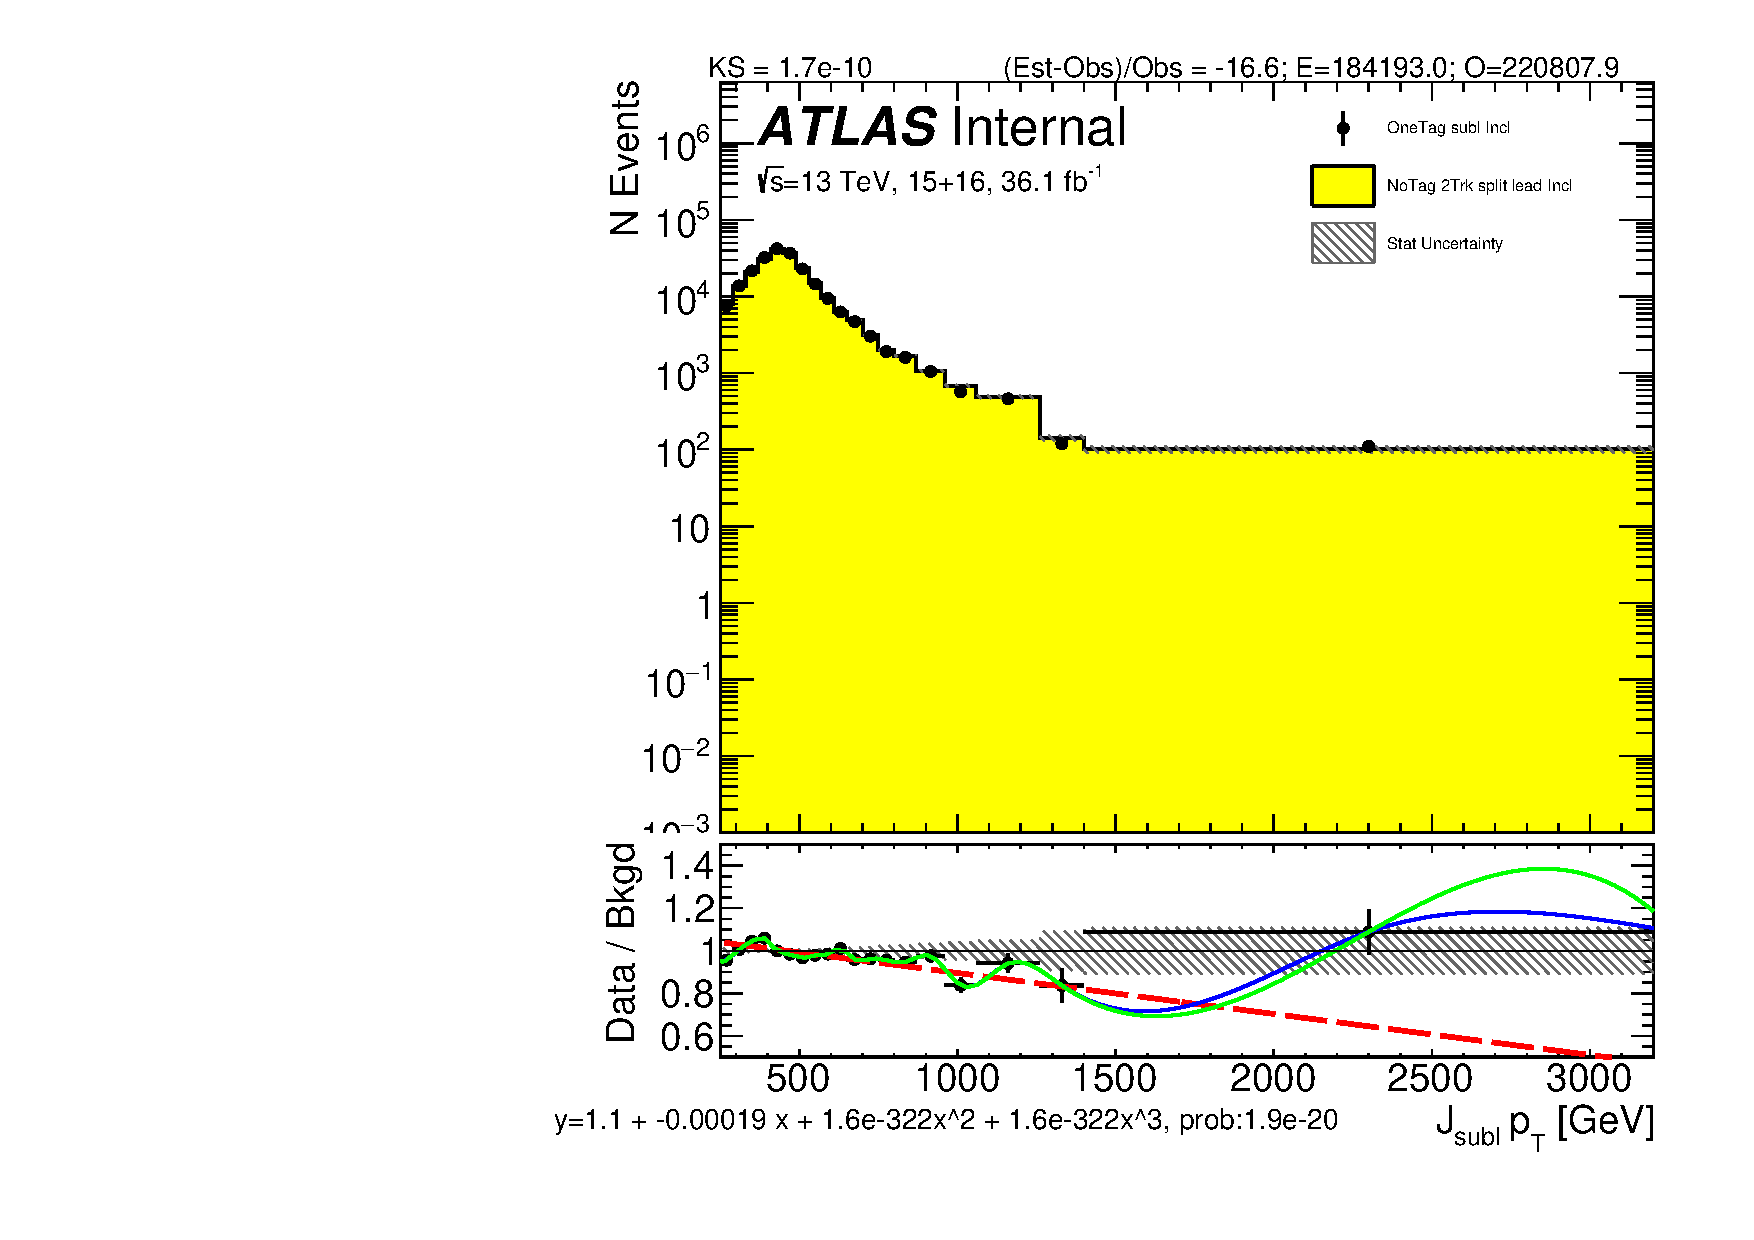
\includegraphics[width=0.25\textwidth,angle=-90]{figures/boosted/Reweight/Fits/Moriond_NoTag_2Trk_split_lead_Incl_sublHCand_Pt_m_1.pdf}
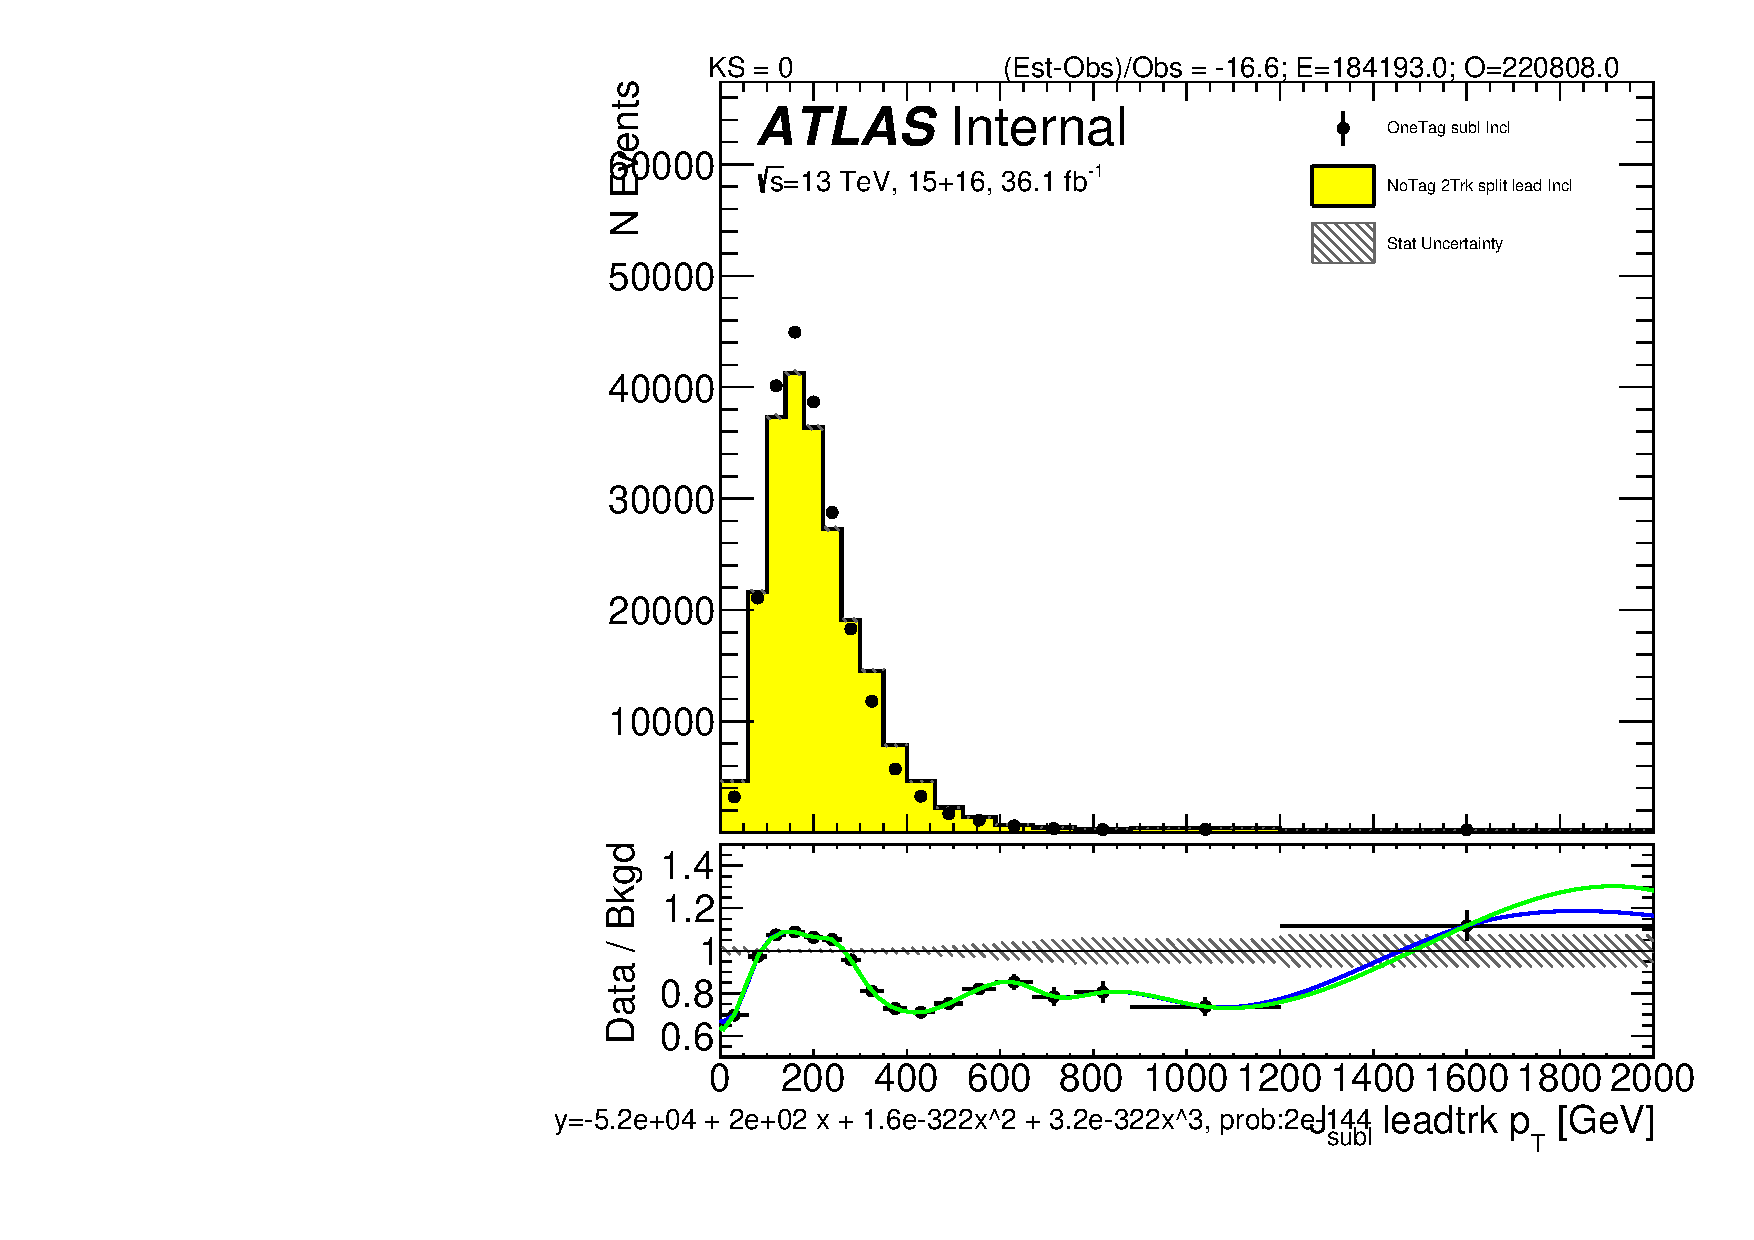
\includegraphics[width=0.25\textwidth,angle=-90]{figures/boosted/Reweight/Fits/Moriond_NoTag_2Trk_split_lead_Incl_sublHCand_trk0_Pt.pdf}
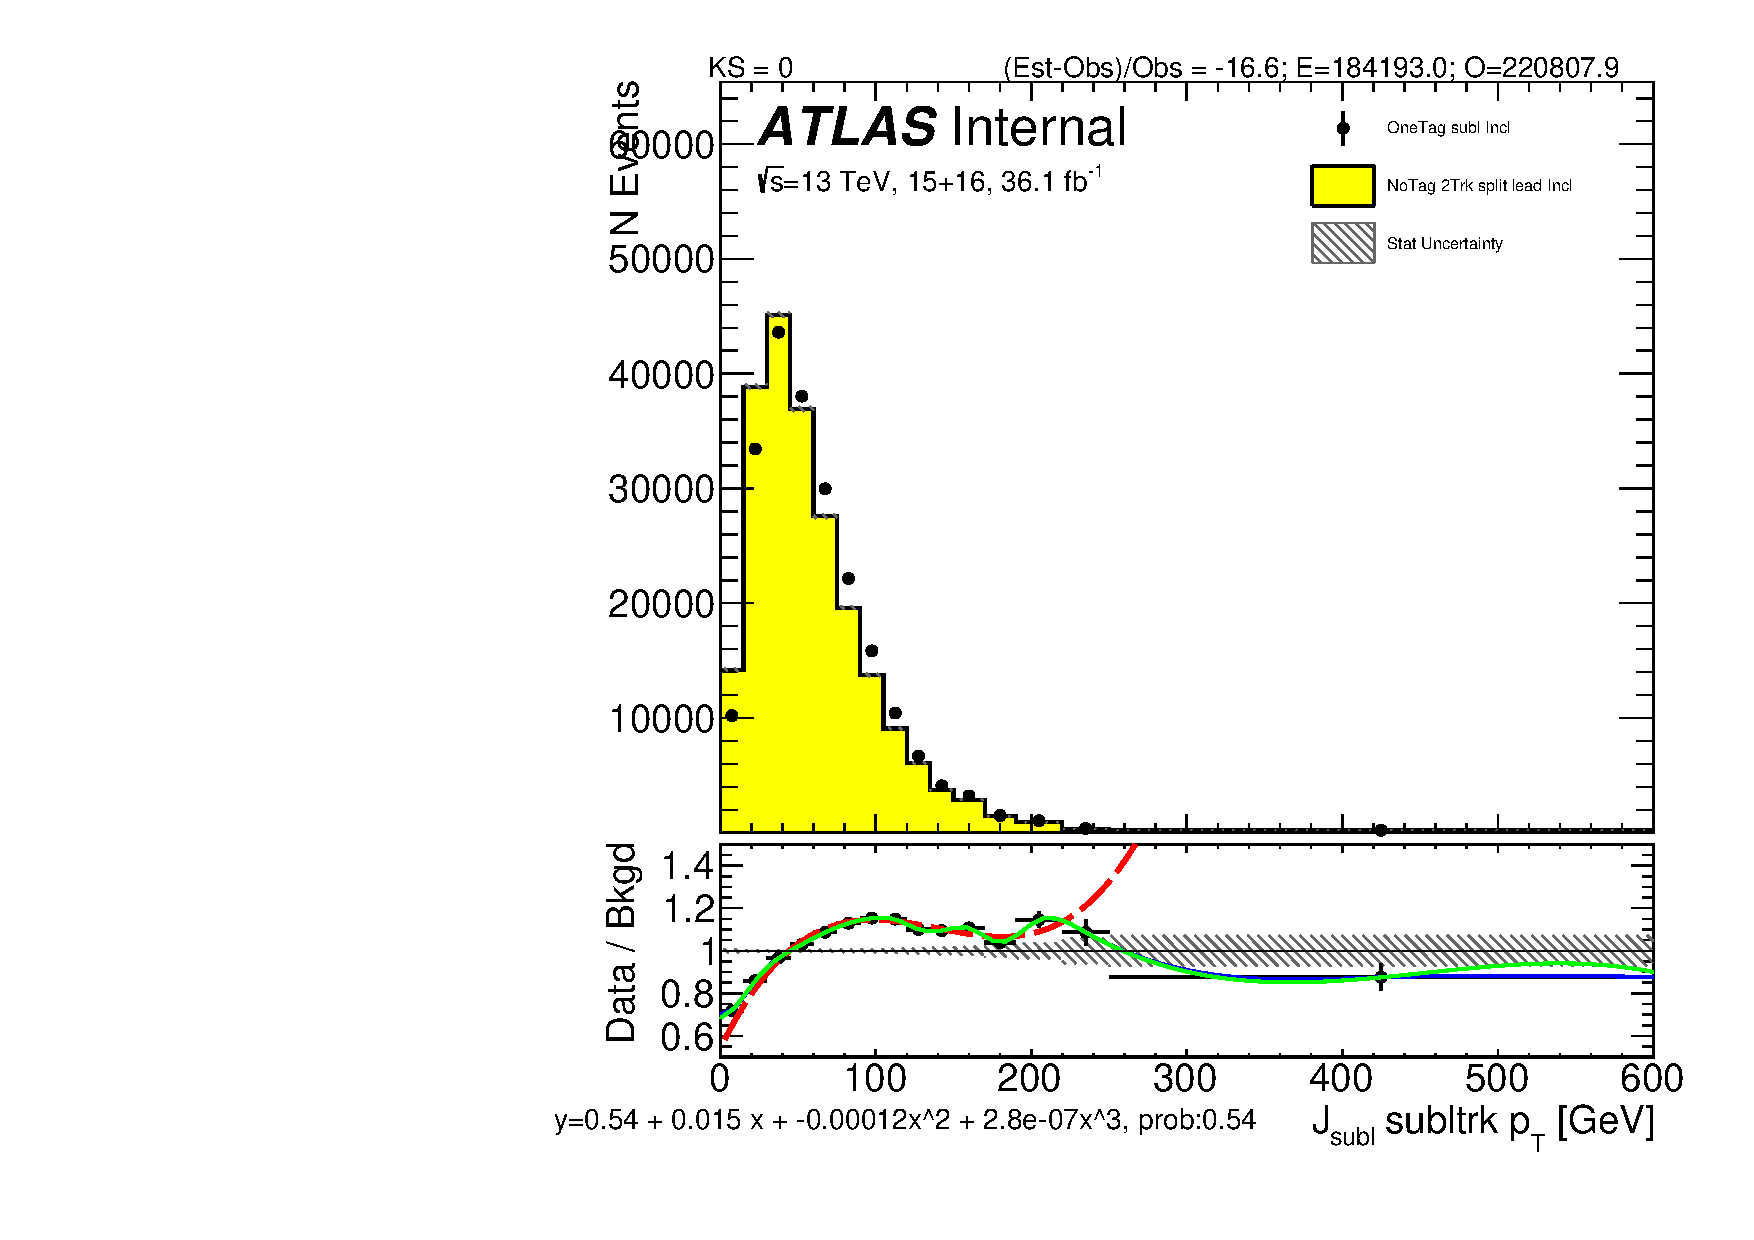
\includegraphics[width=0.25\textwidth,angle=-90]{figures/boosted/Reweight/Fits/Moriond_NoTag_2Trk_split_lead_Incl_sublHCand_trk1_Pt.pdf} \\
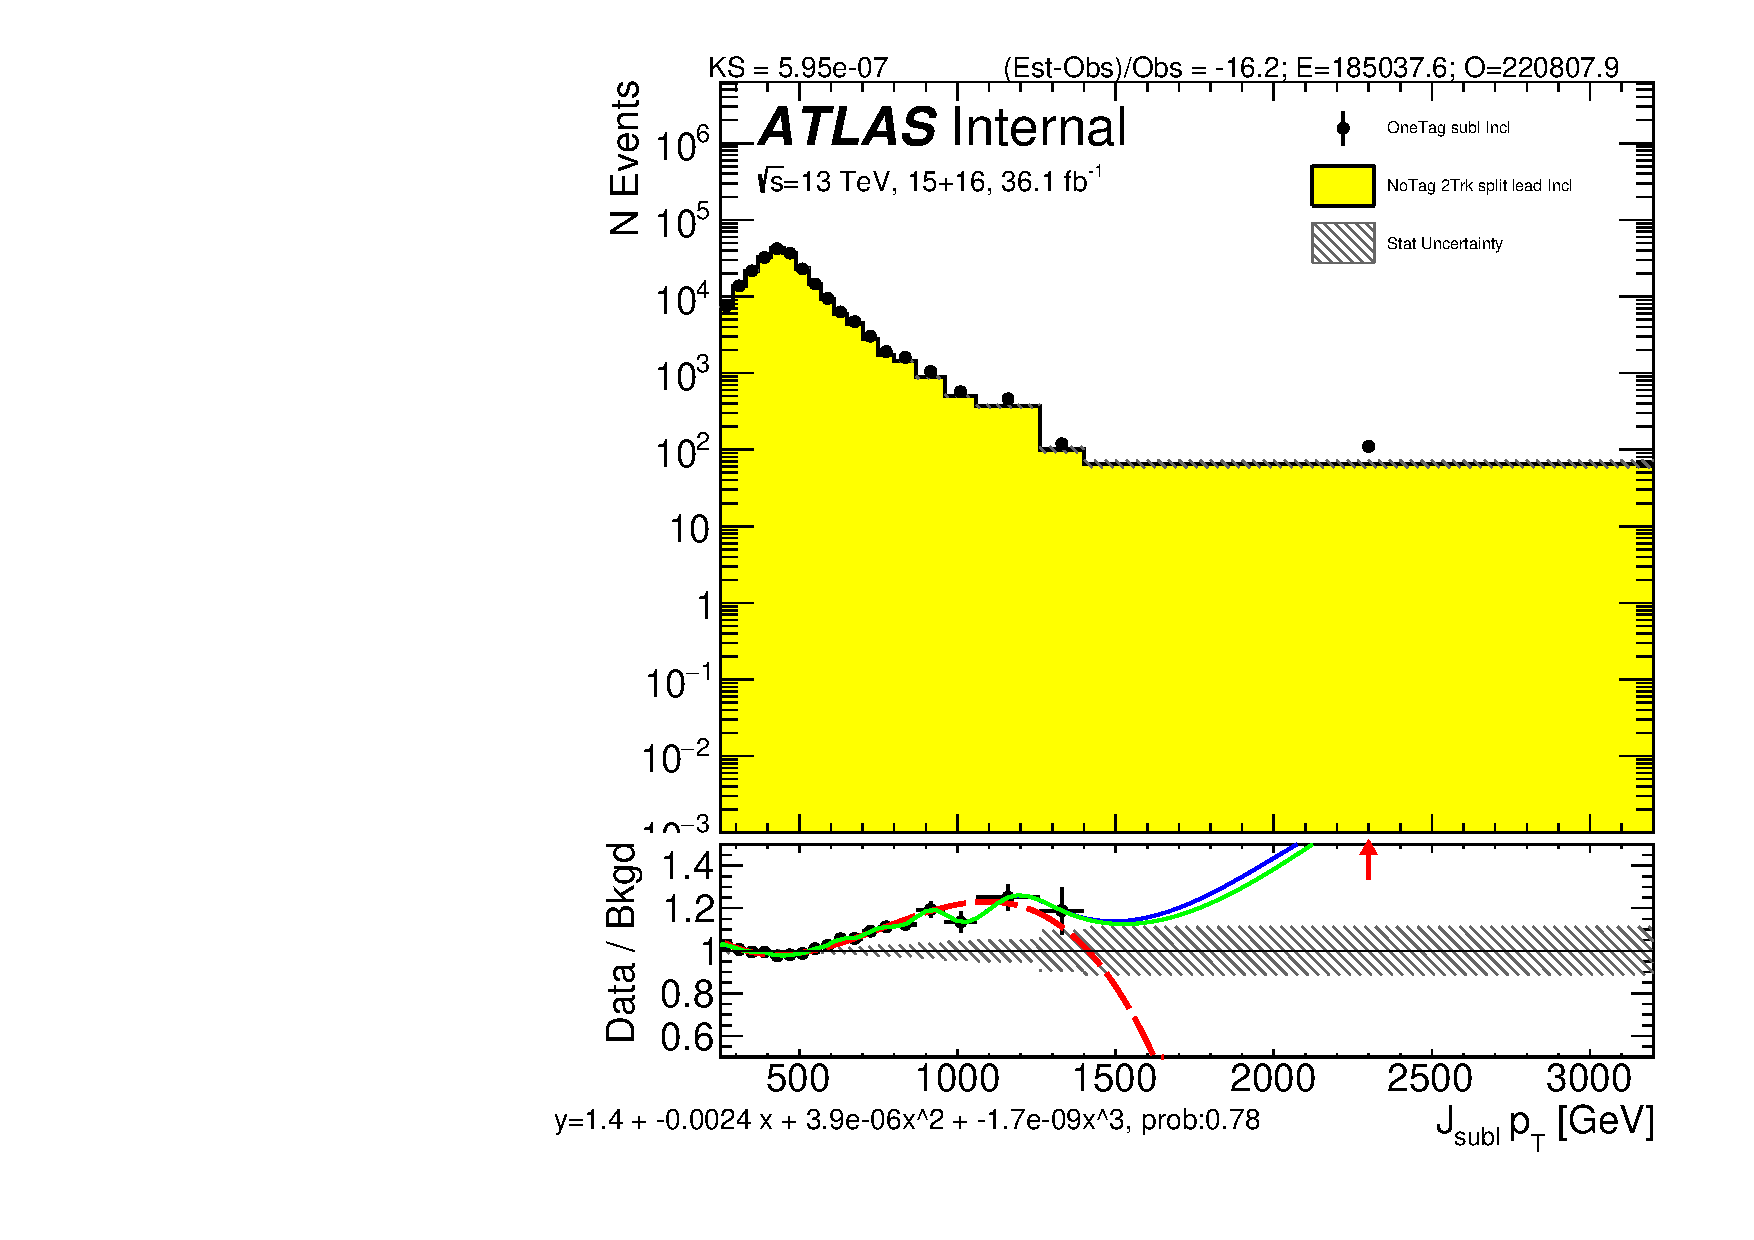
\includegraphics[width=0.25\textwidth,angle=-90]{figures/boosted/Reweight/Fits/Moriond_bkg_0_NoTag_2Trk_split_lead_Incl_sublHCand_Pt_m_1.pdf}
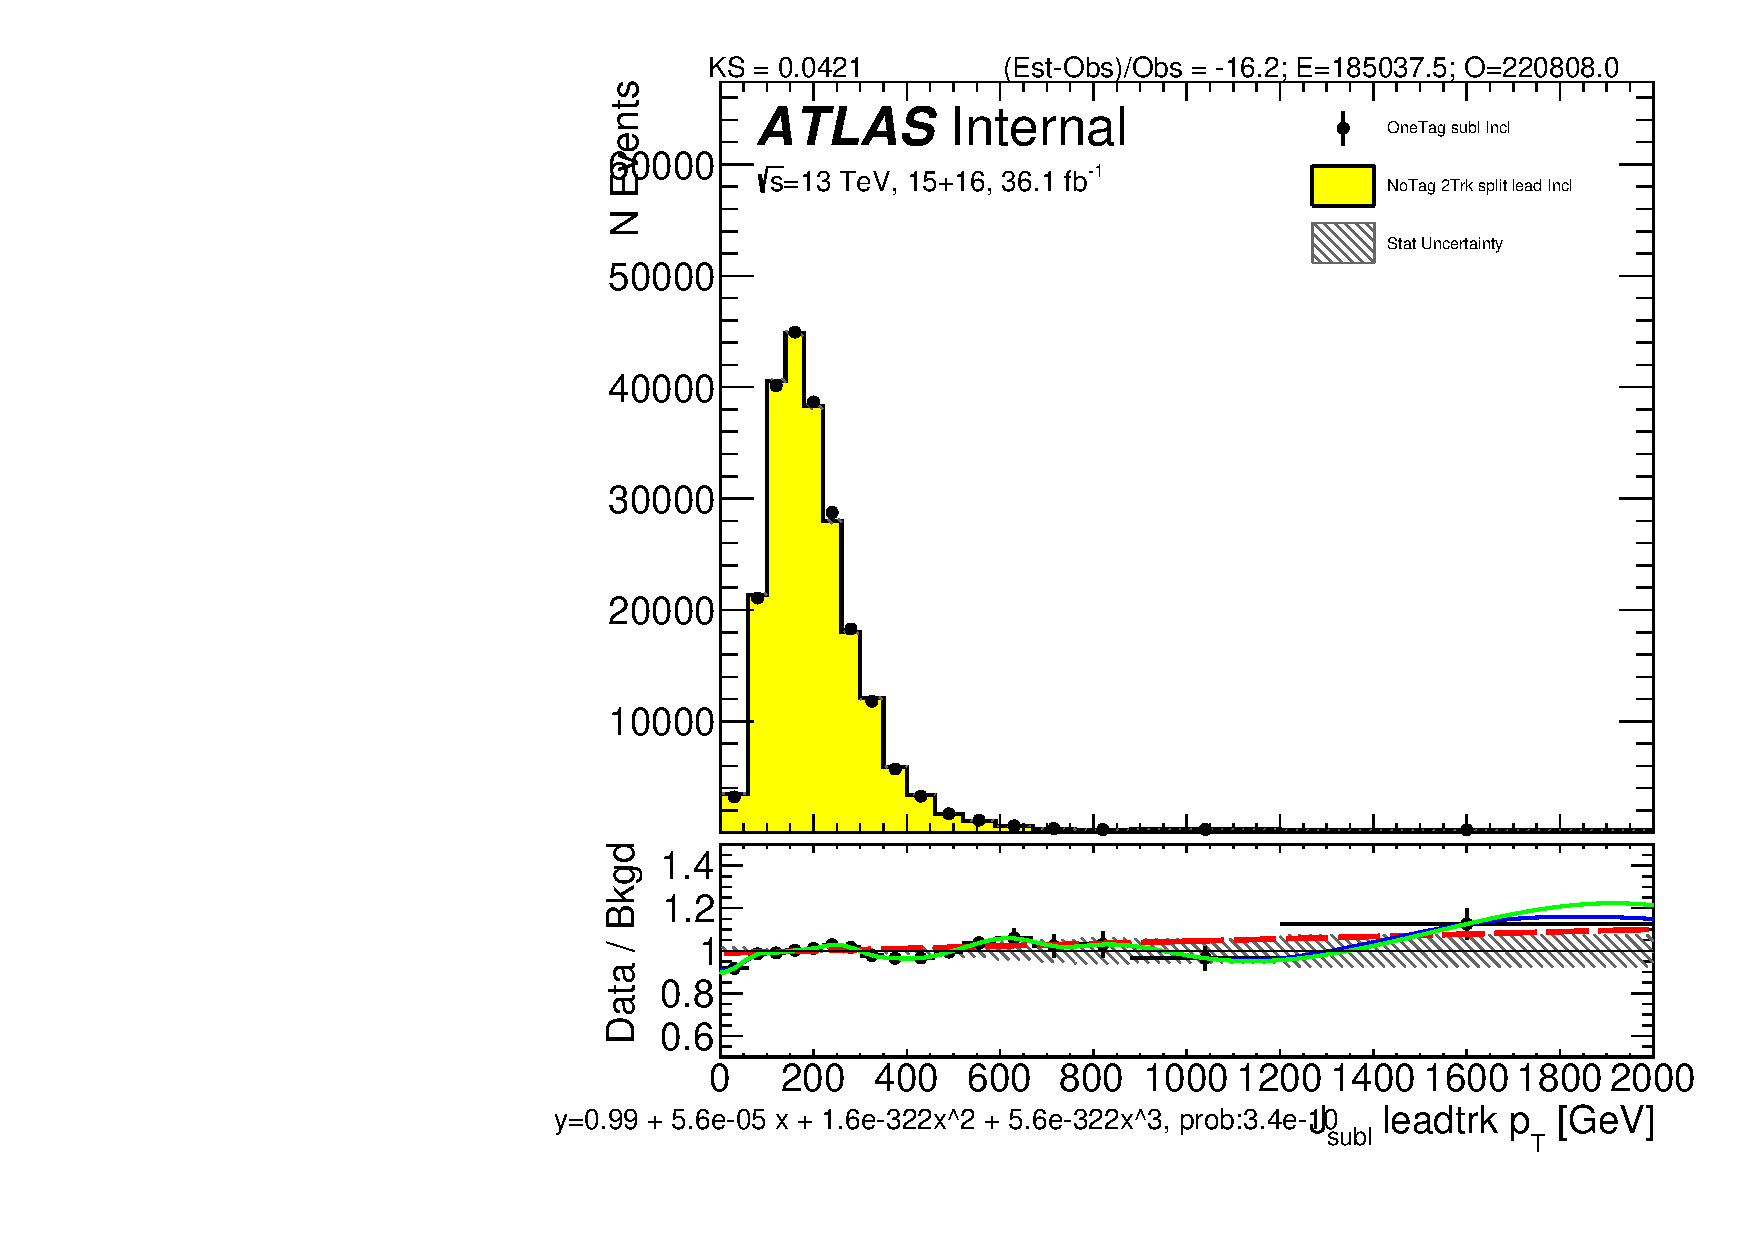
\includegraphics[width=0.25\textwidth,angle=-90]{figures/boosted/Reweight/Fits/Moriond_bkg_0_NoTag_2Trk_split_lead_Incl_sublHCand_trk0_Pt.pdf}
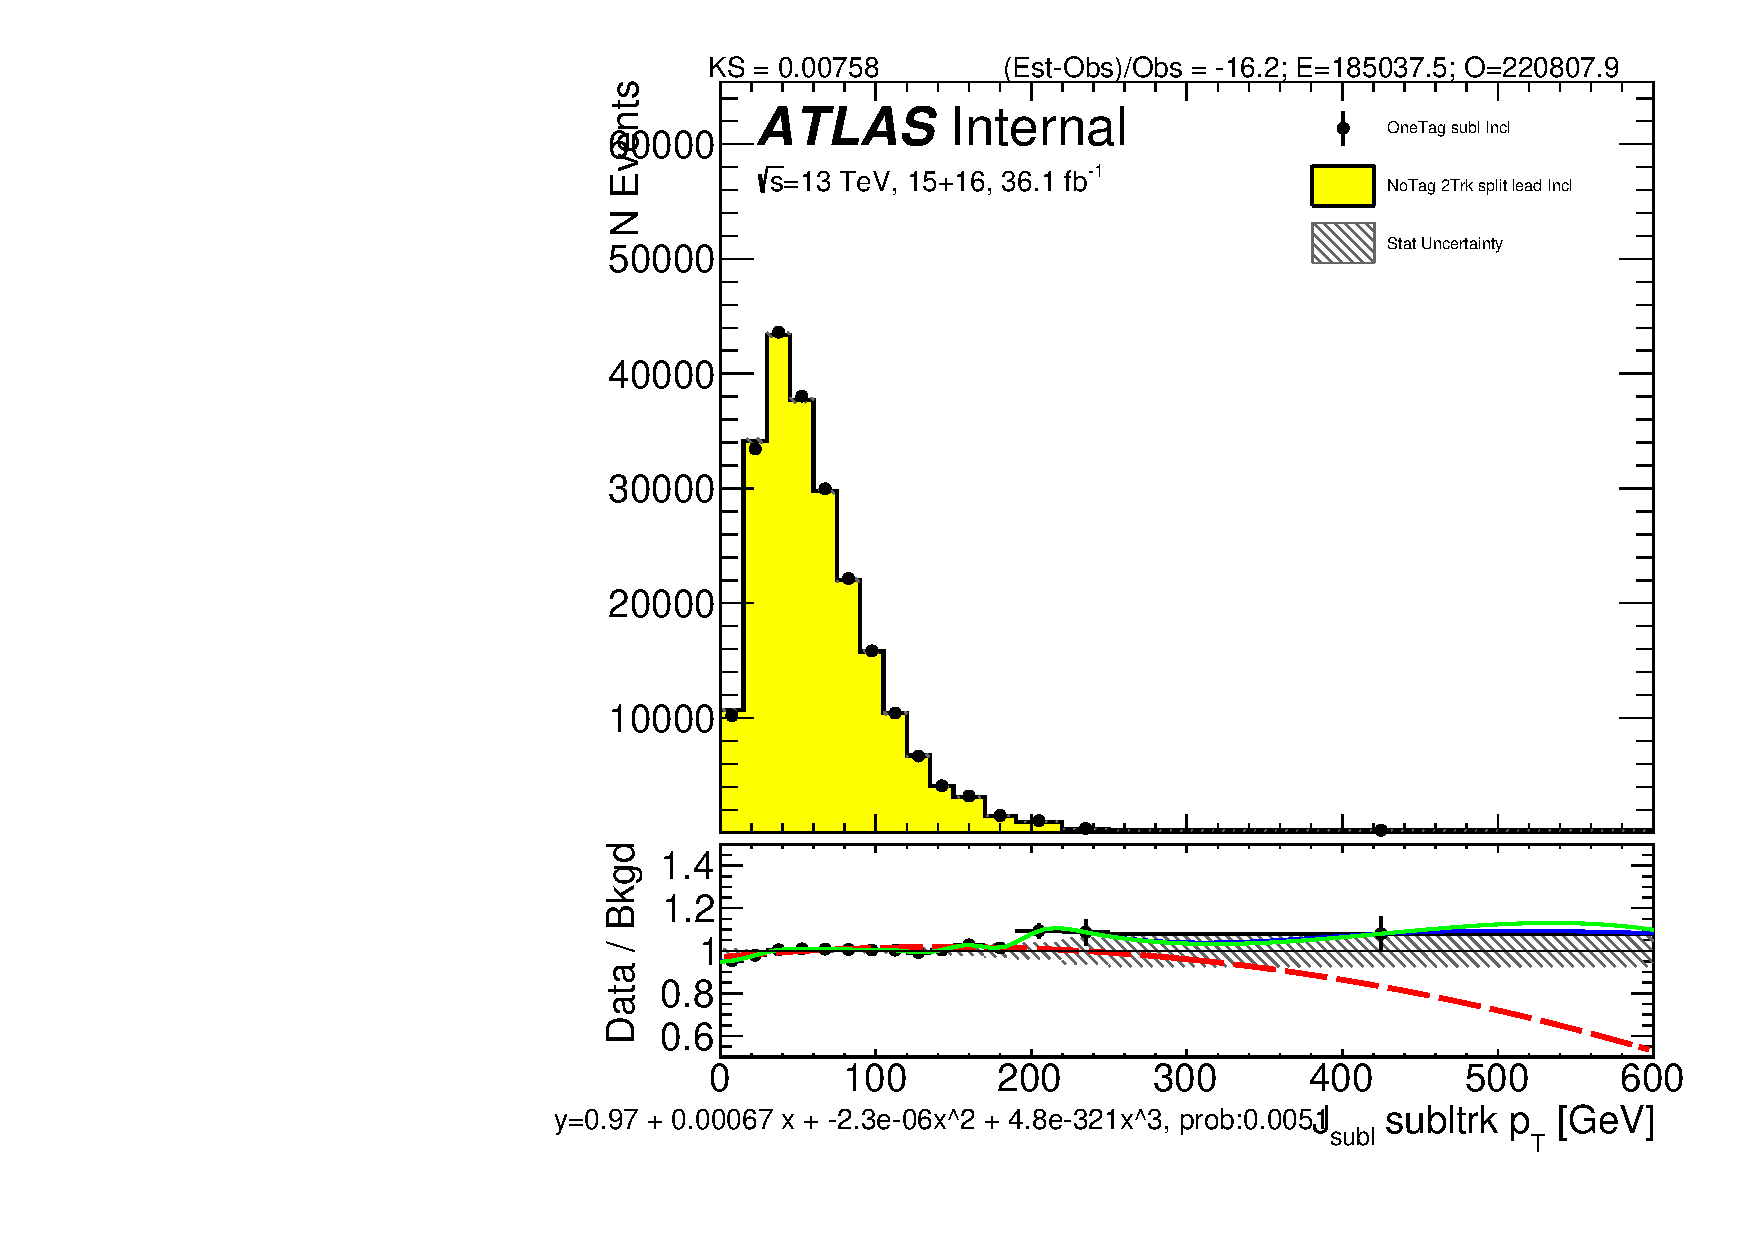
\includegraphics[width=0.25\textwidth,angle=-90]{figures/boosted/Reweight/Fits/Moriond_bkg_0_NoTag_2Trk_split_lead_Incl_sublHCand_trk1_Pt.pdf} \\
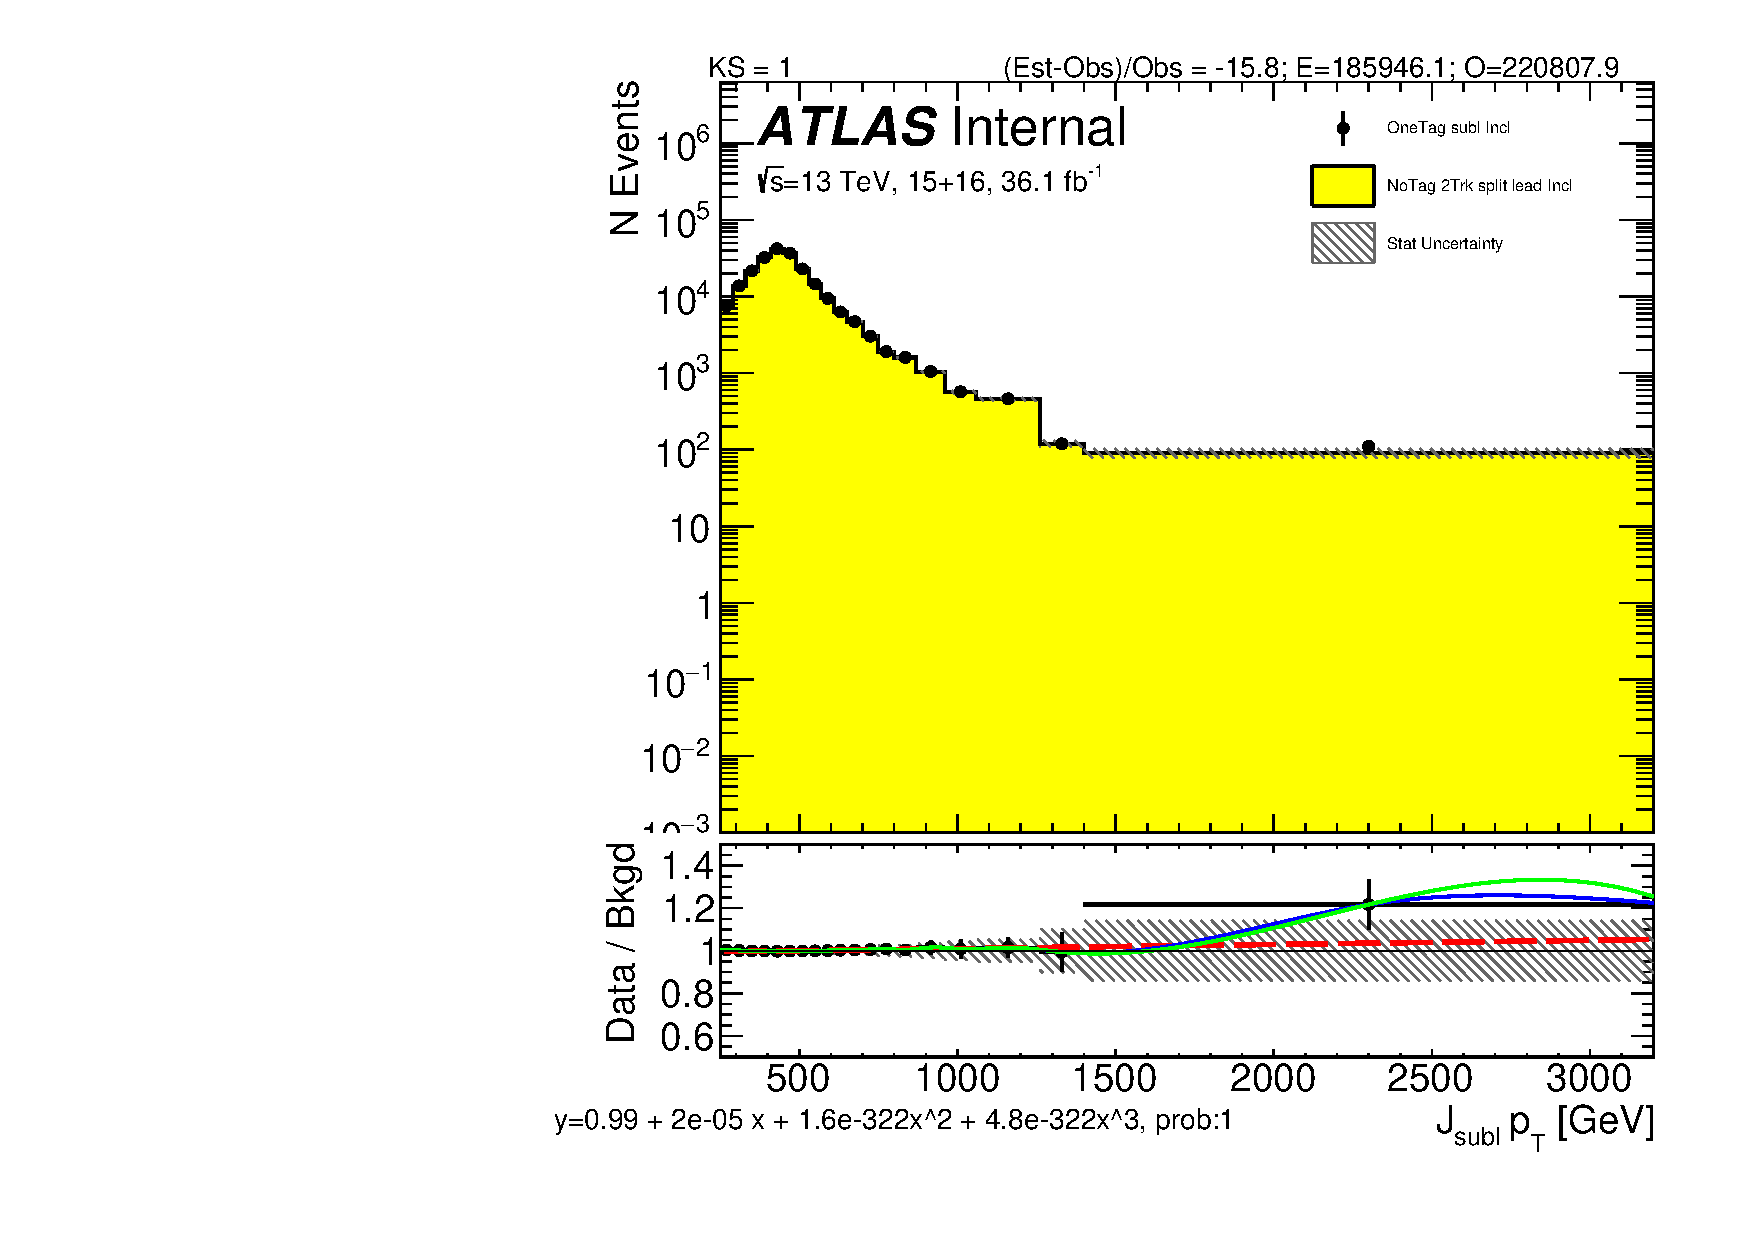
\includegraphics[width=0.25\textwidth,angle=-90]{figures/boosted/Reweight/Fits/Moriond_bkg_3_NoTag_2Trk_split_lead_Incl_sublHCand_Pt_m_1.pdf}
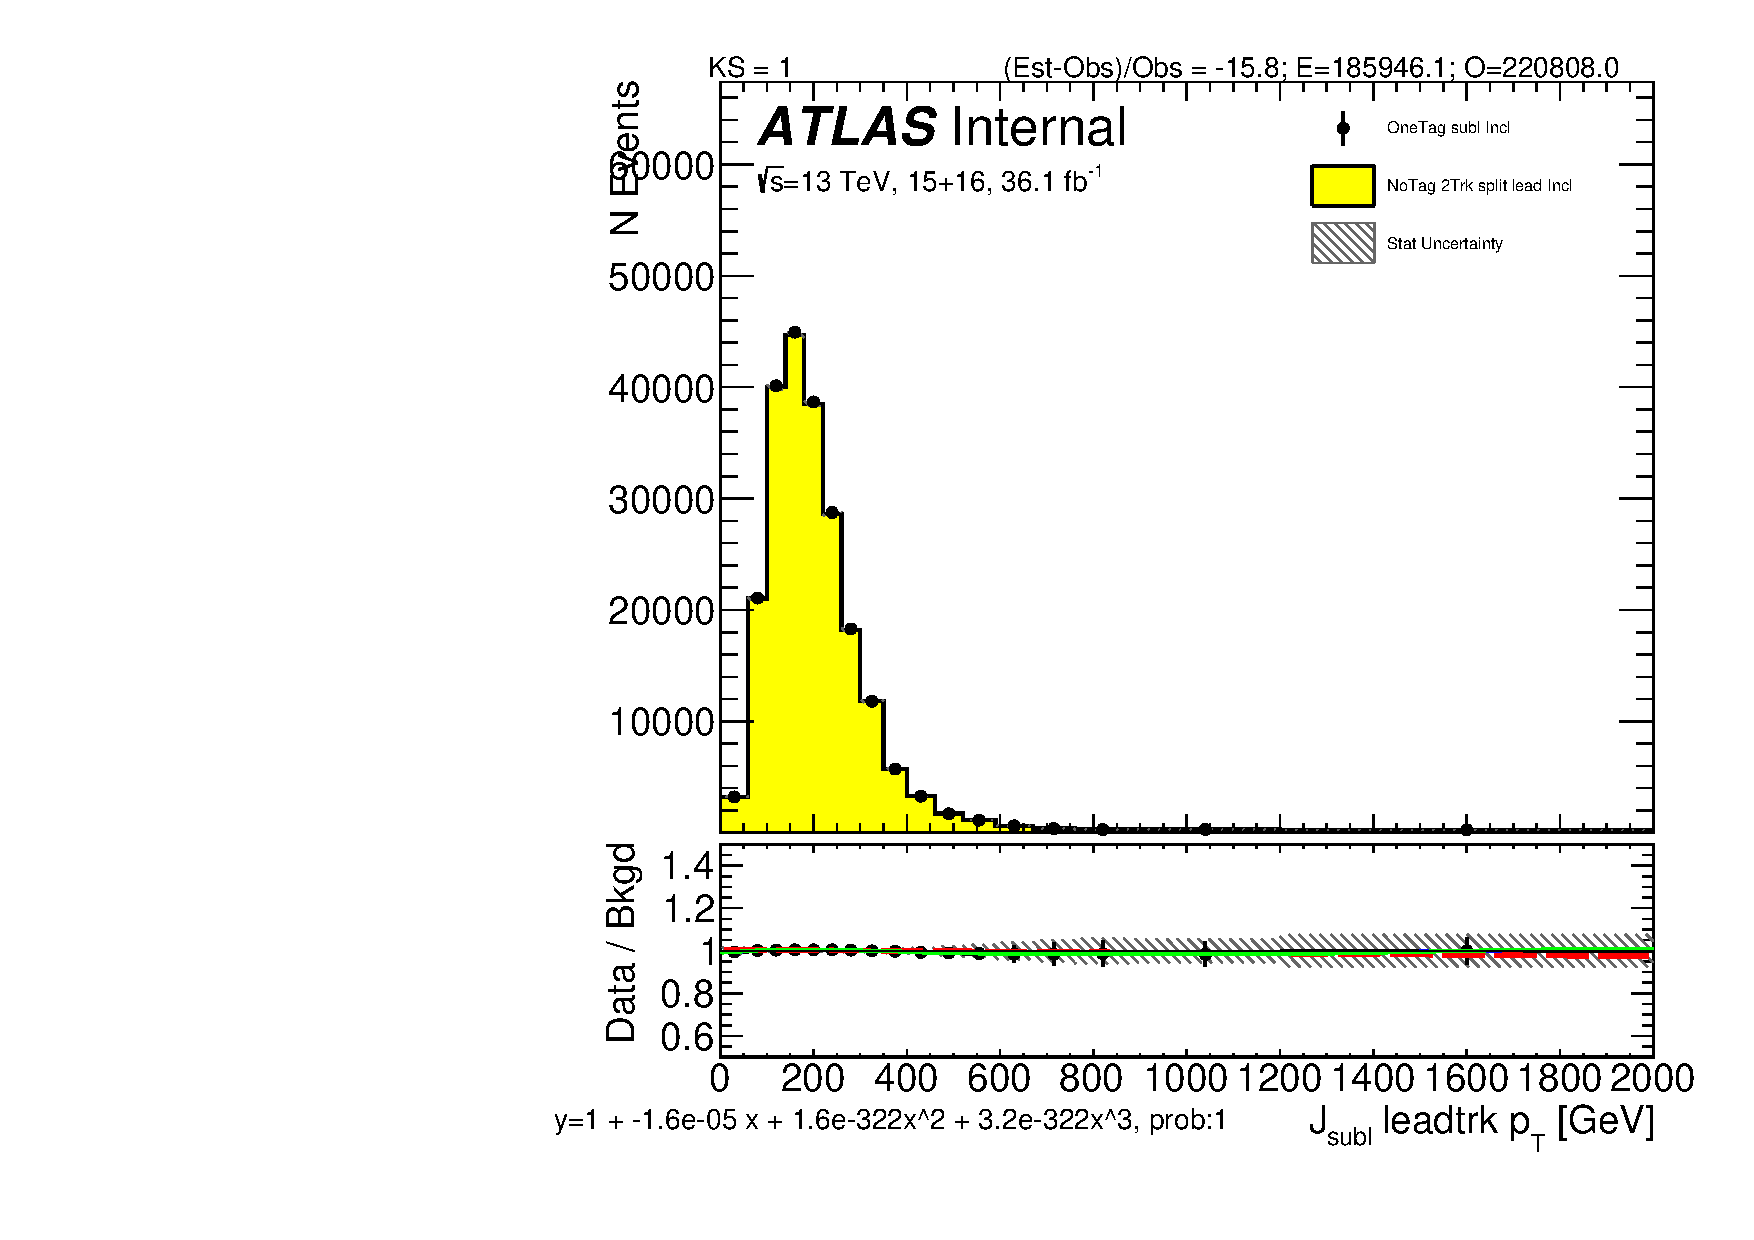
\includegraphics[width=0.25\textwidth,angle=-90]{figures/boosted/Reweight/Fits/Moriond_bkg_3_NoTag_2Trk_split_lead_Incl_sublHCand_trk0_Pt.pdf}
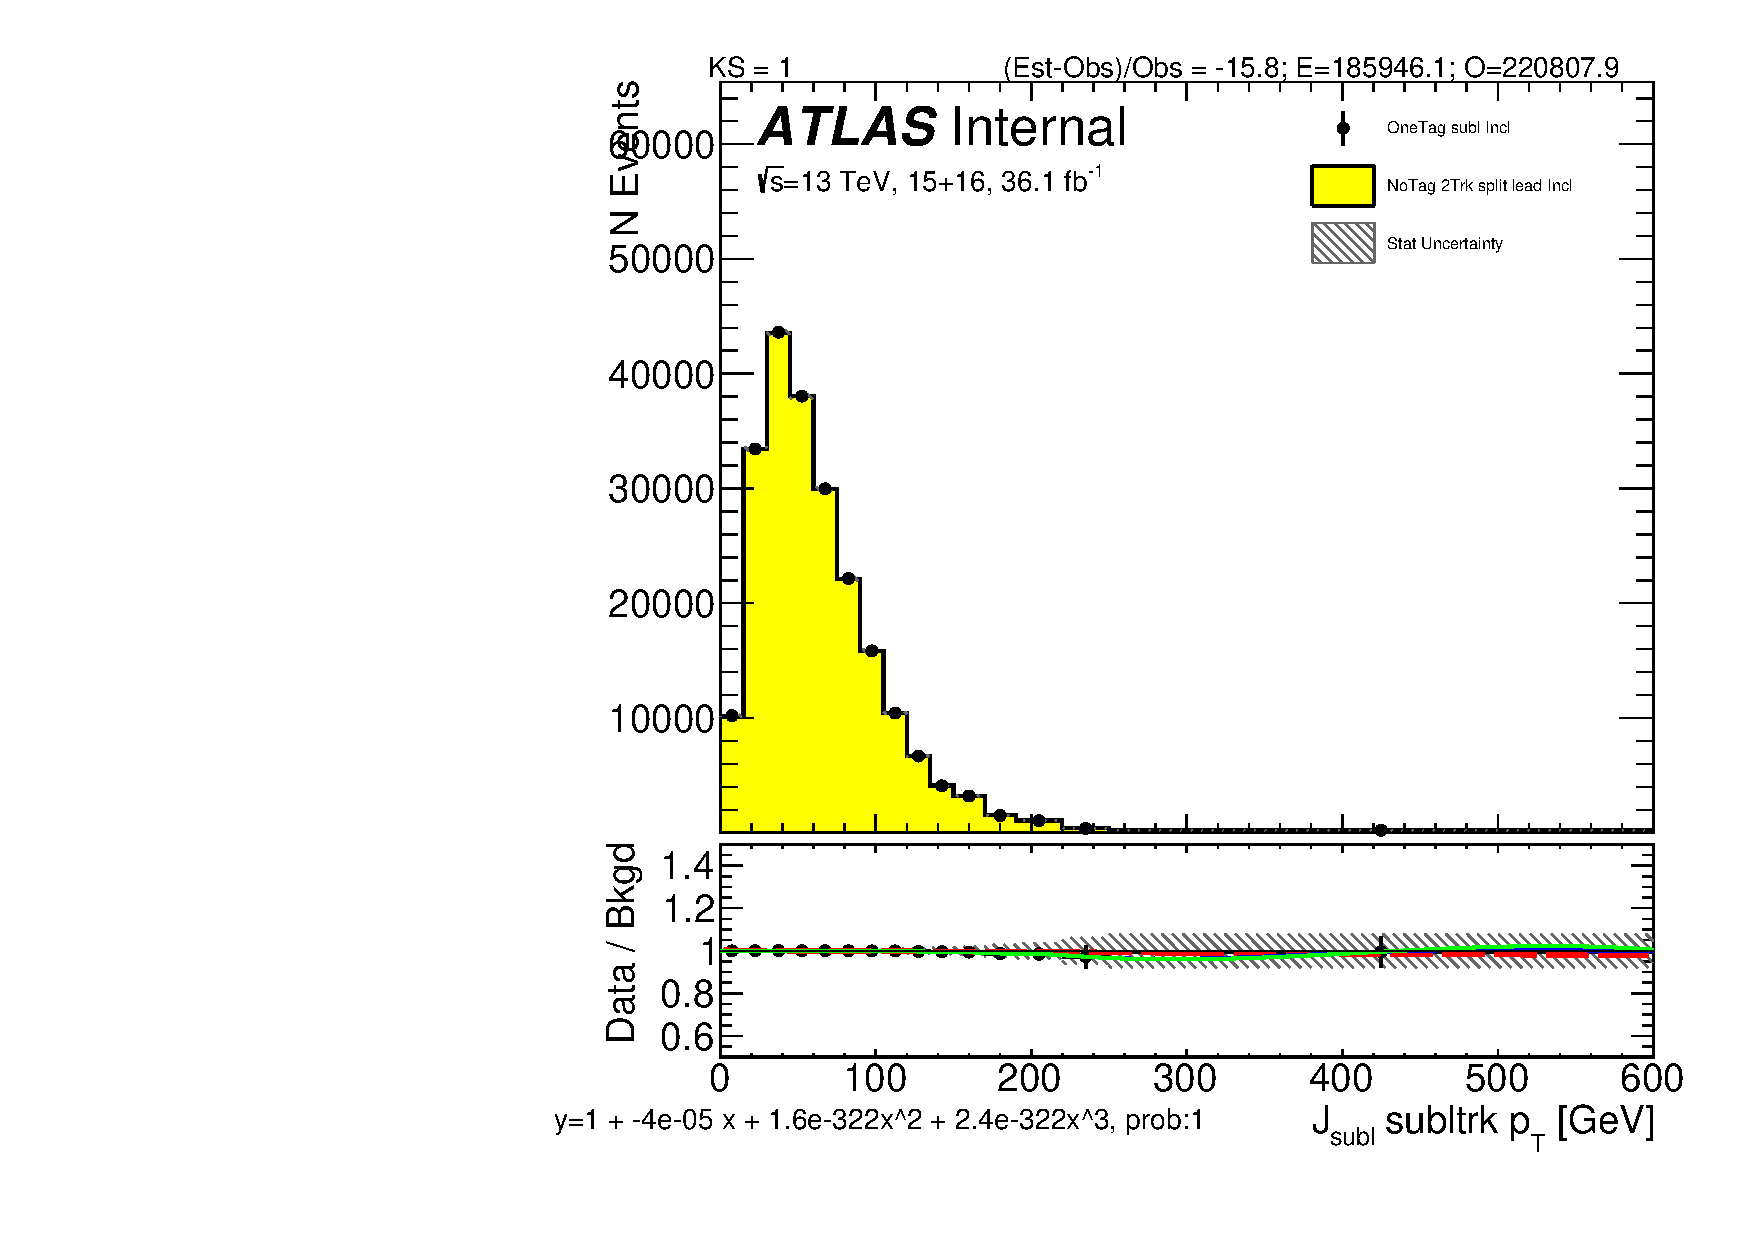
\includegraphics[width=0.25\textwidth,angle=-90]{figures/boosted/Reweight/Fits/Moriond_bkg_3_NoTag_2Trk_split_lead_Incl_sublHCand_trk1_Pt.pdf} \\
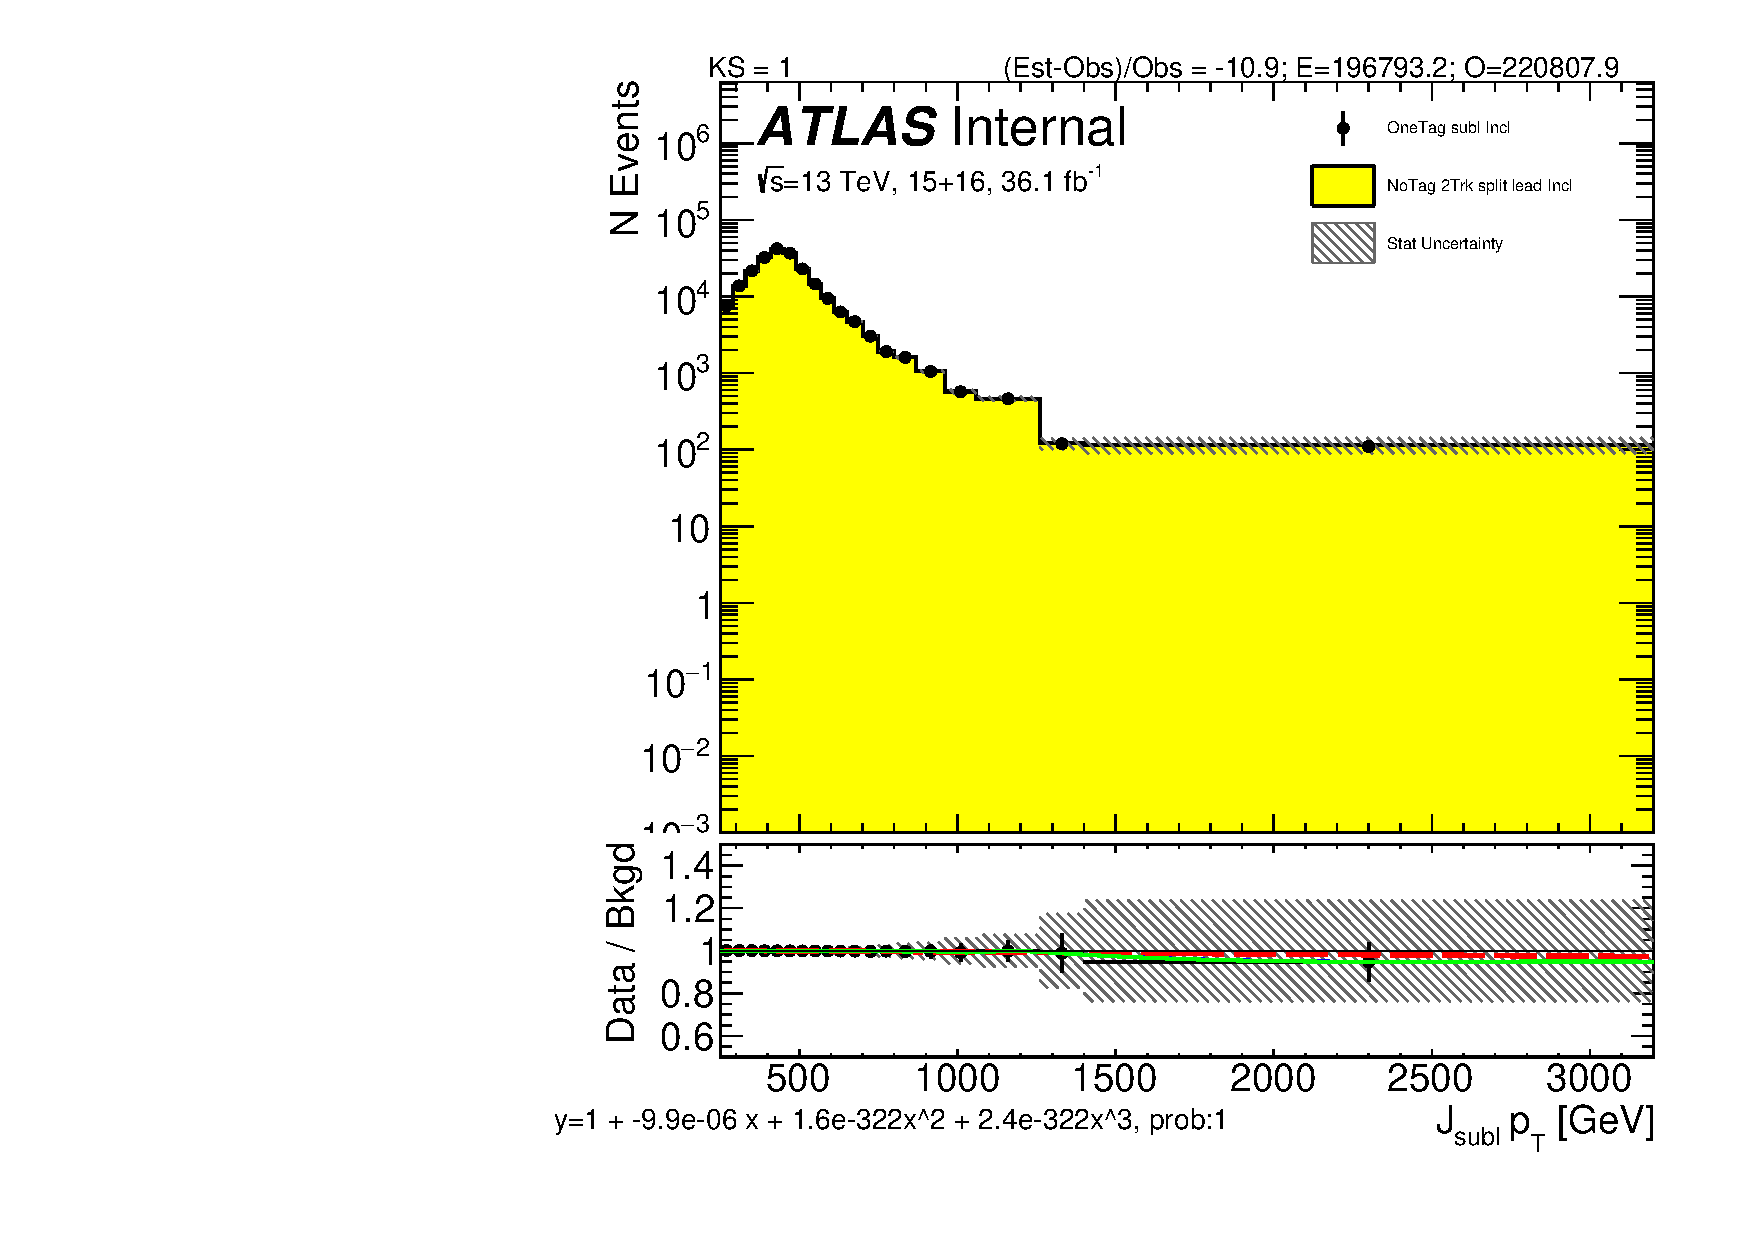
\includegraphics[width=0.25\textwidth,angle=-90]{figures/boosted/Reweight/Fits/Moriond_bkg_9_NoTag_2Trk_split_lead_Incl_sublHCand_Pt_m_1.pdf}
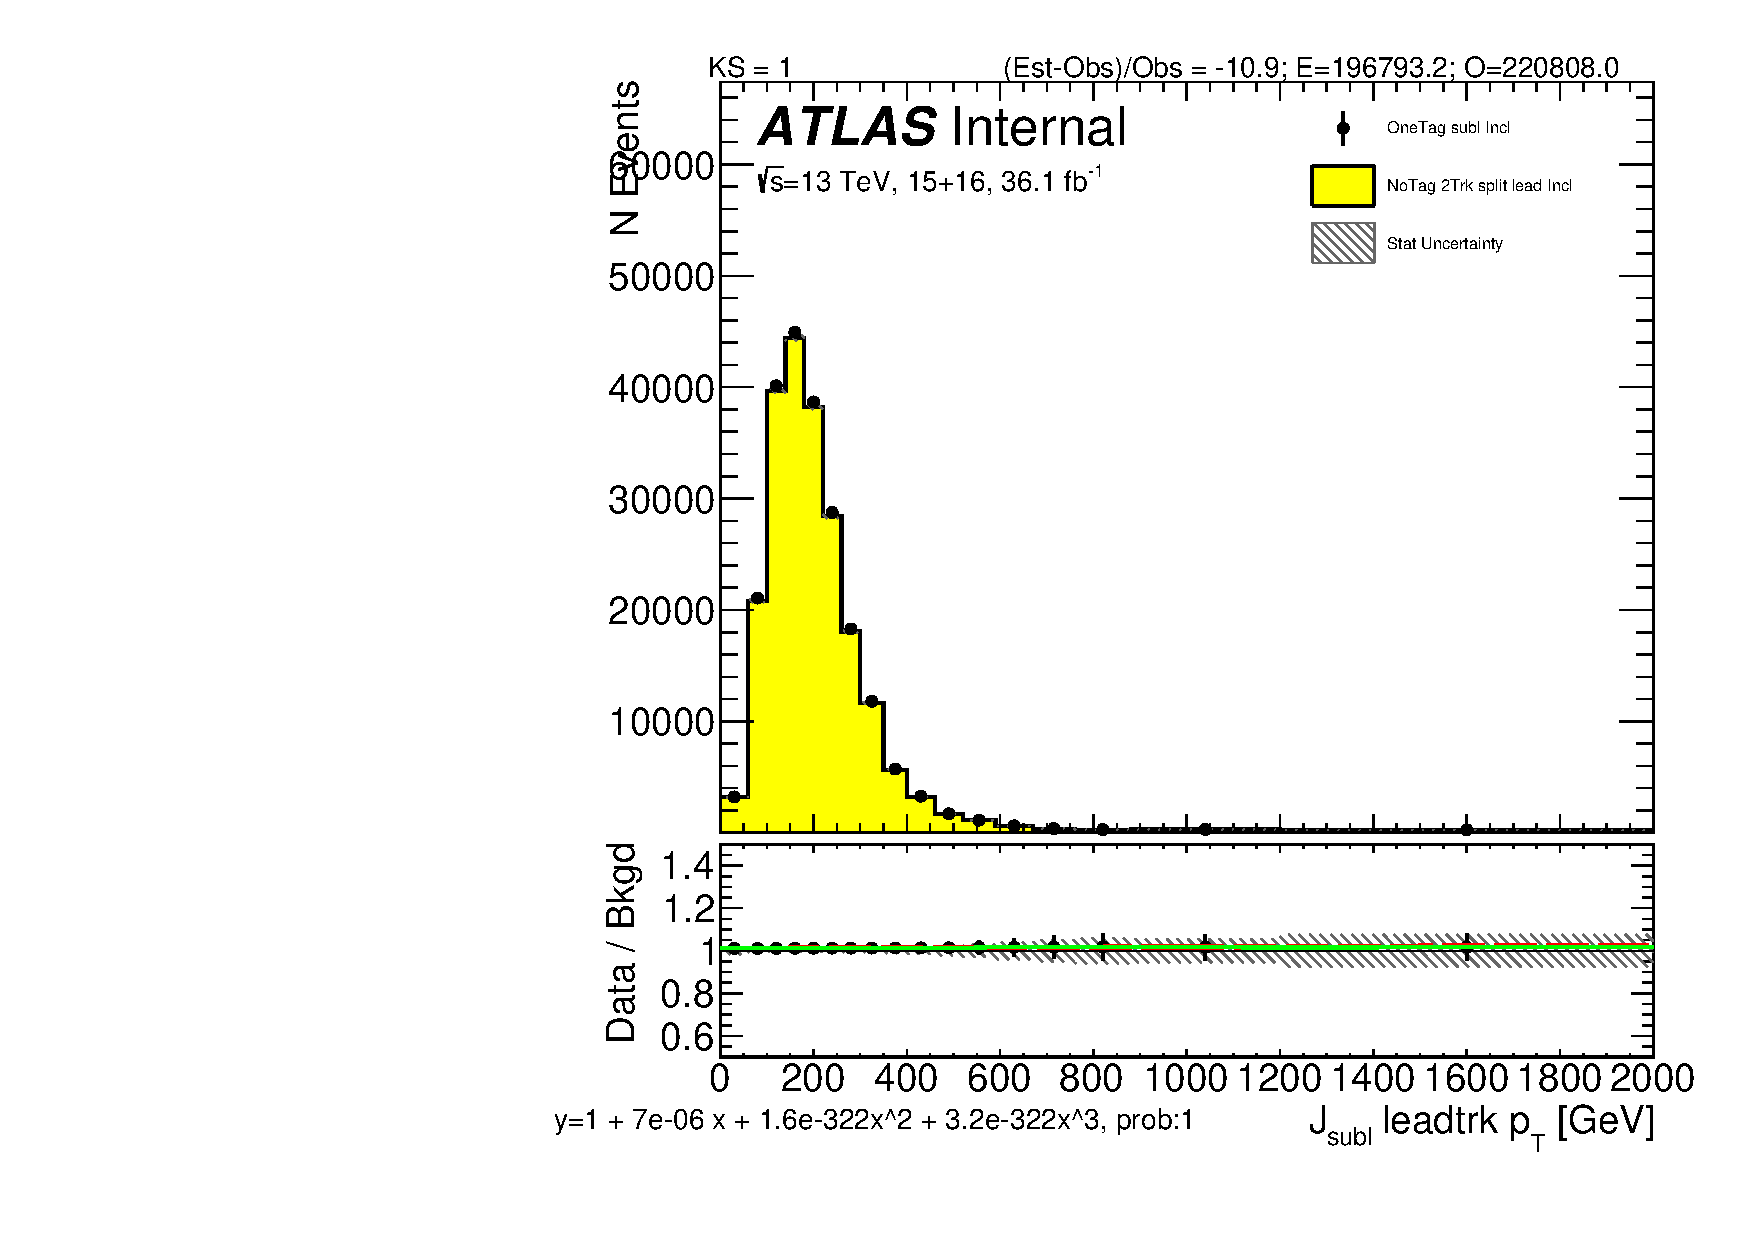
\includegraphics[width=0.25\textwidth,angle=-90]{figures/boosted/Reweight/Fits/Moriond_bkg_9_NoTag_2Trk_split_lead_Incl_sublHCand_trk0_Pt.pdf}
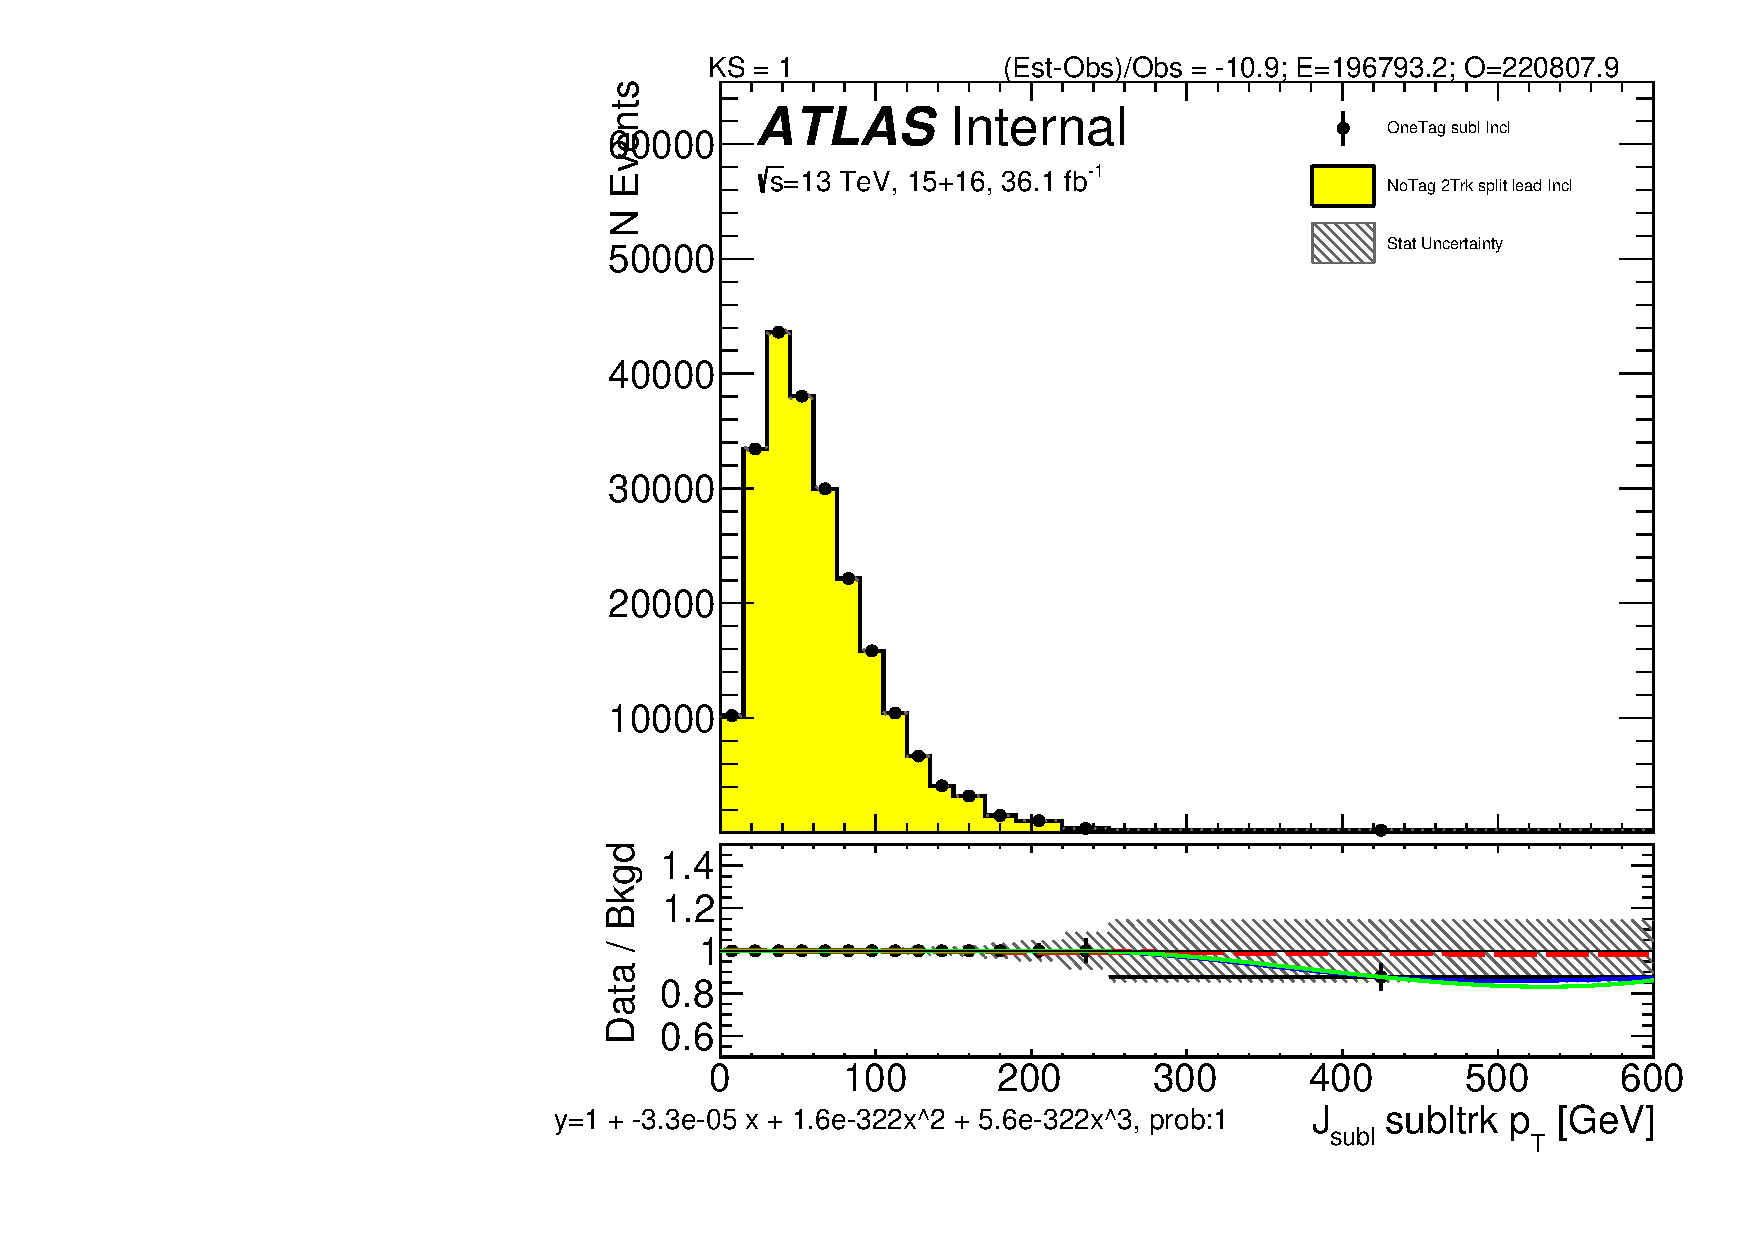
\includegraphics[width=0.25\textwidth,angle=-90]{figures/boosted/Reweight/Fits/Moriond_bkg_9_NoTag_2Trk_split_lead_Incl_sublHCand_trk1_Pt.pdf} \\
\caption{For $2bs$ background estimate: the fits to the ratio of the data in the $1b$ category, of the subleading Higgs candidate $1b$-tagged events's subleading Higgs candidate distributions(black point), over the leading Higgs candidate $1b$-tagged events's subleading Higgs candidate distributions(yellow). Distributions and fits to the estimated QCD background for large-\R jet $p_{T}$ (left), the large-\R jet's leading trackjet $p_T$ (middle), and large-\R jet's subleading trackjet $p_T$ (right) are shown.  Figures are before reweighting (top row), after the first iteration(second row), after the fourth iteration(third row), and after the last iteration (bottom row). The green line is the spline fit; the red line is a polynomial fit; the blue line is the spline interpolation.}
\label{fig:rw-2bs-lead}
\end{center}
\end{figure*}

\begin{figure*}[htbp!]
\begin{center}
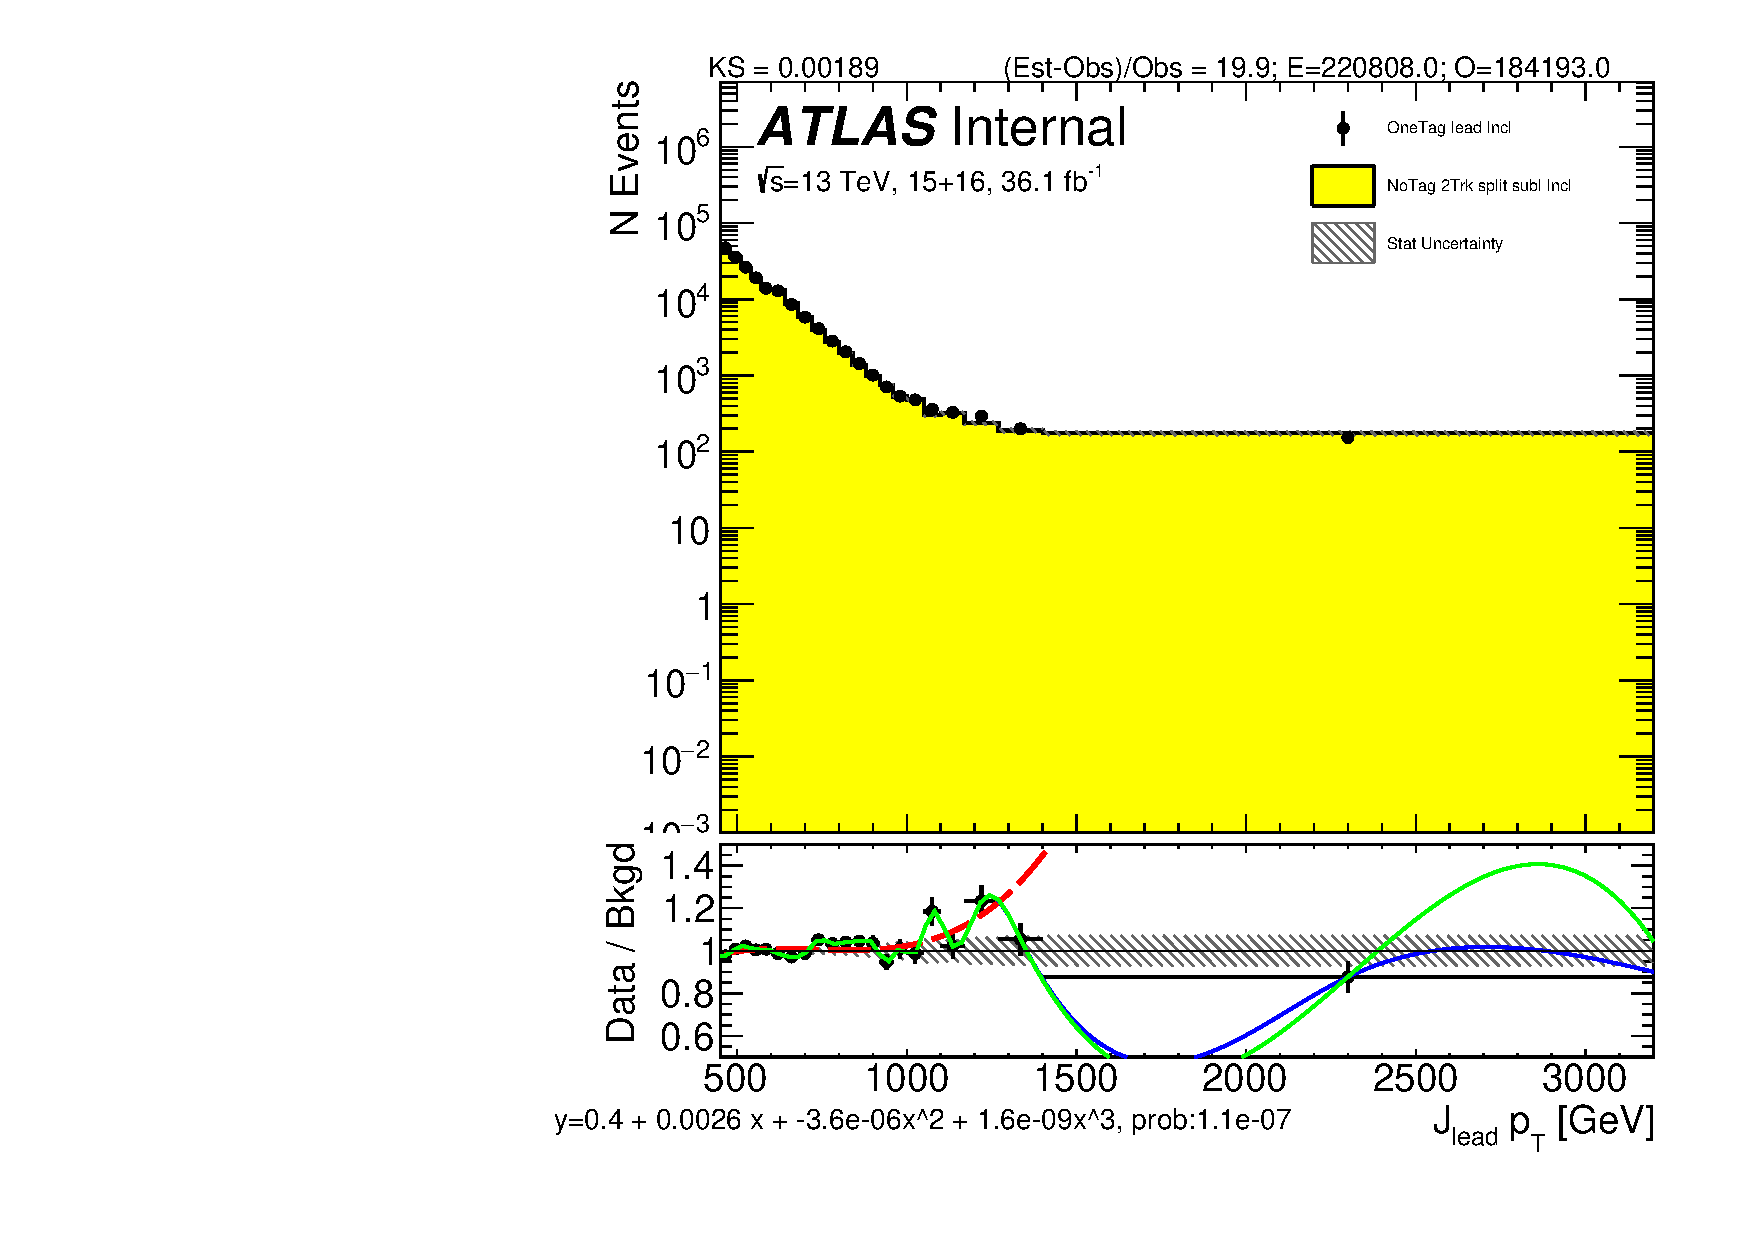
\includegraphics[width=0.25\textwidth,angle=-90]{figures/boosted/Reweight/Fits/Moriond_NoTag_2Trk_split_subl_Incl_leadHCand_Pt_m_1.pdf}
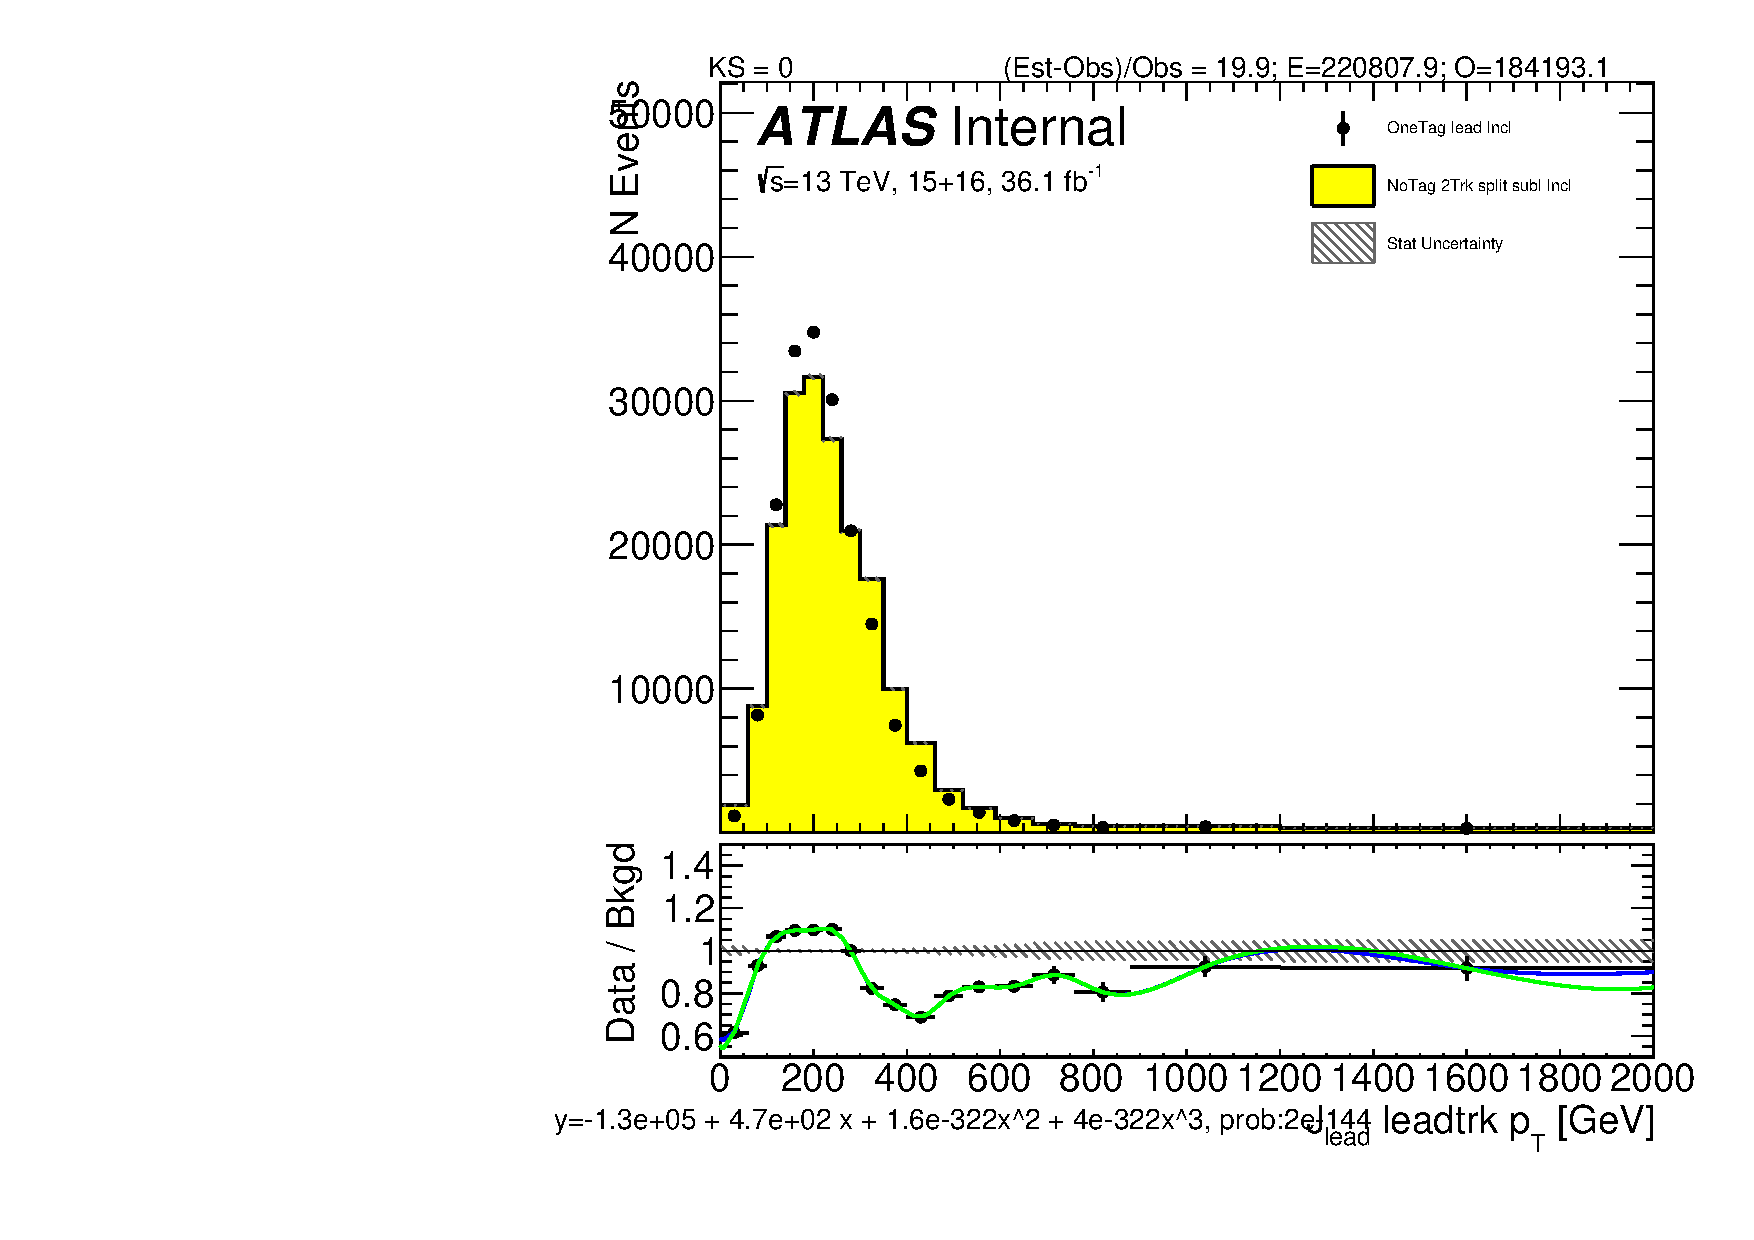
\includegraphics[width=0.25\textwidth,angle=-90]{figures/boosted/Reweight/Fits/Moriond_NoTag_2Trk_split_subl_Incl_leadHCand_trk0_Pt.pdf}
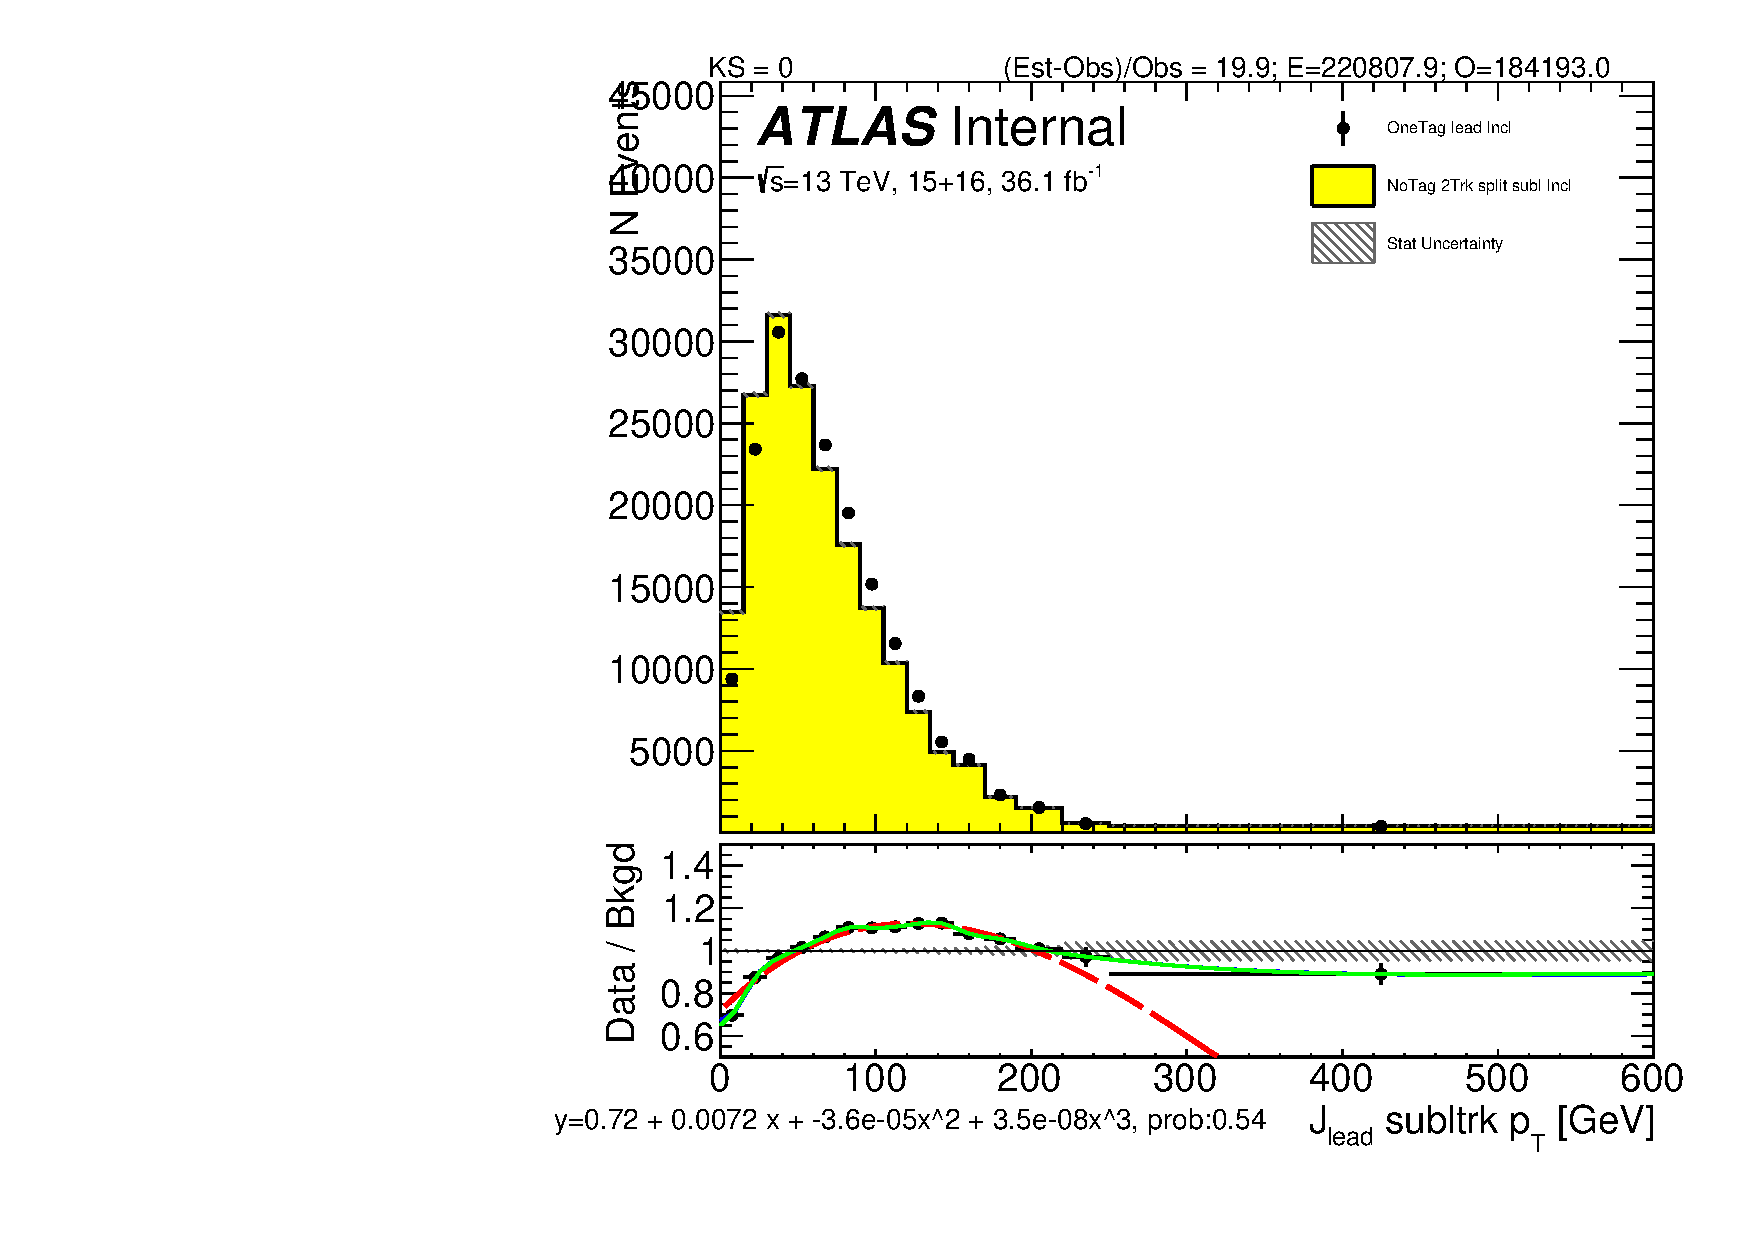
\includegraphics[width=0.25\textwidth,angle=-90]{figures/boosted/Reweight/Fits/Moriond_NoTag_2Trk_split_subl_Incl_leadHCand_trk1_Pt.pdf} \\
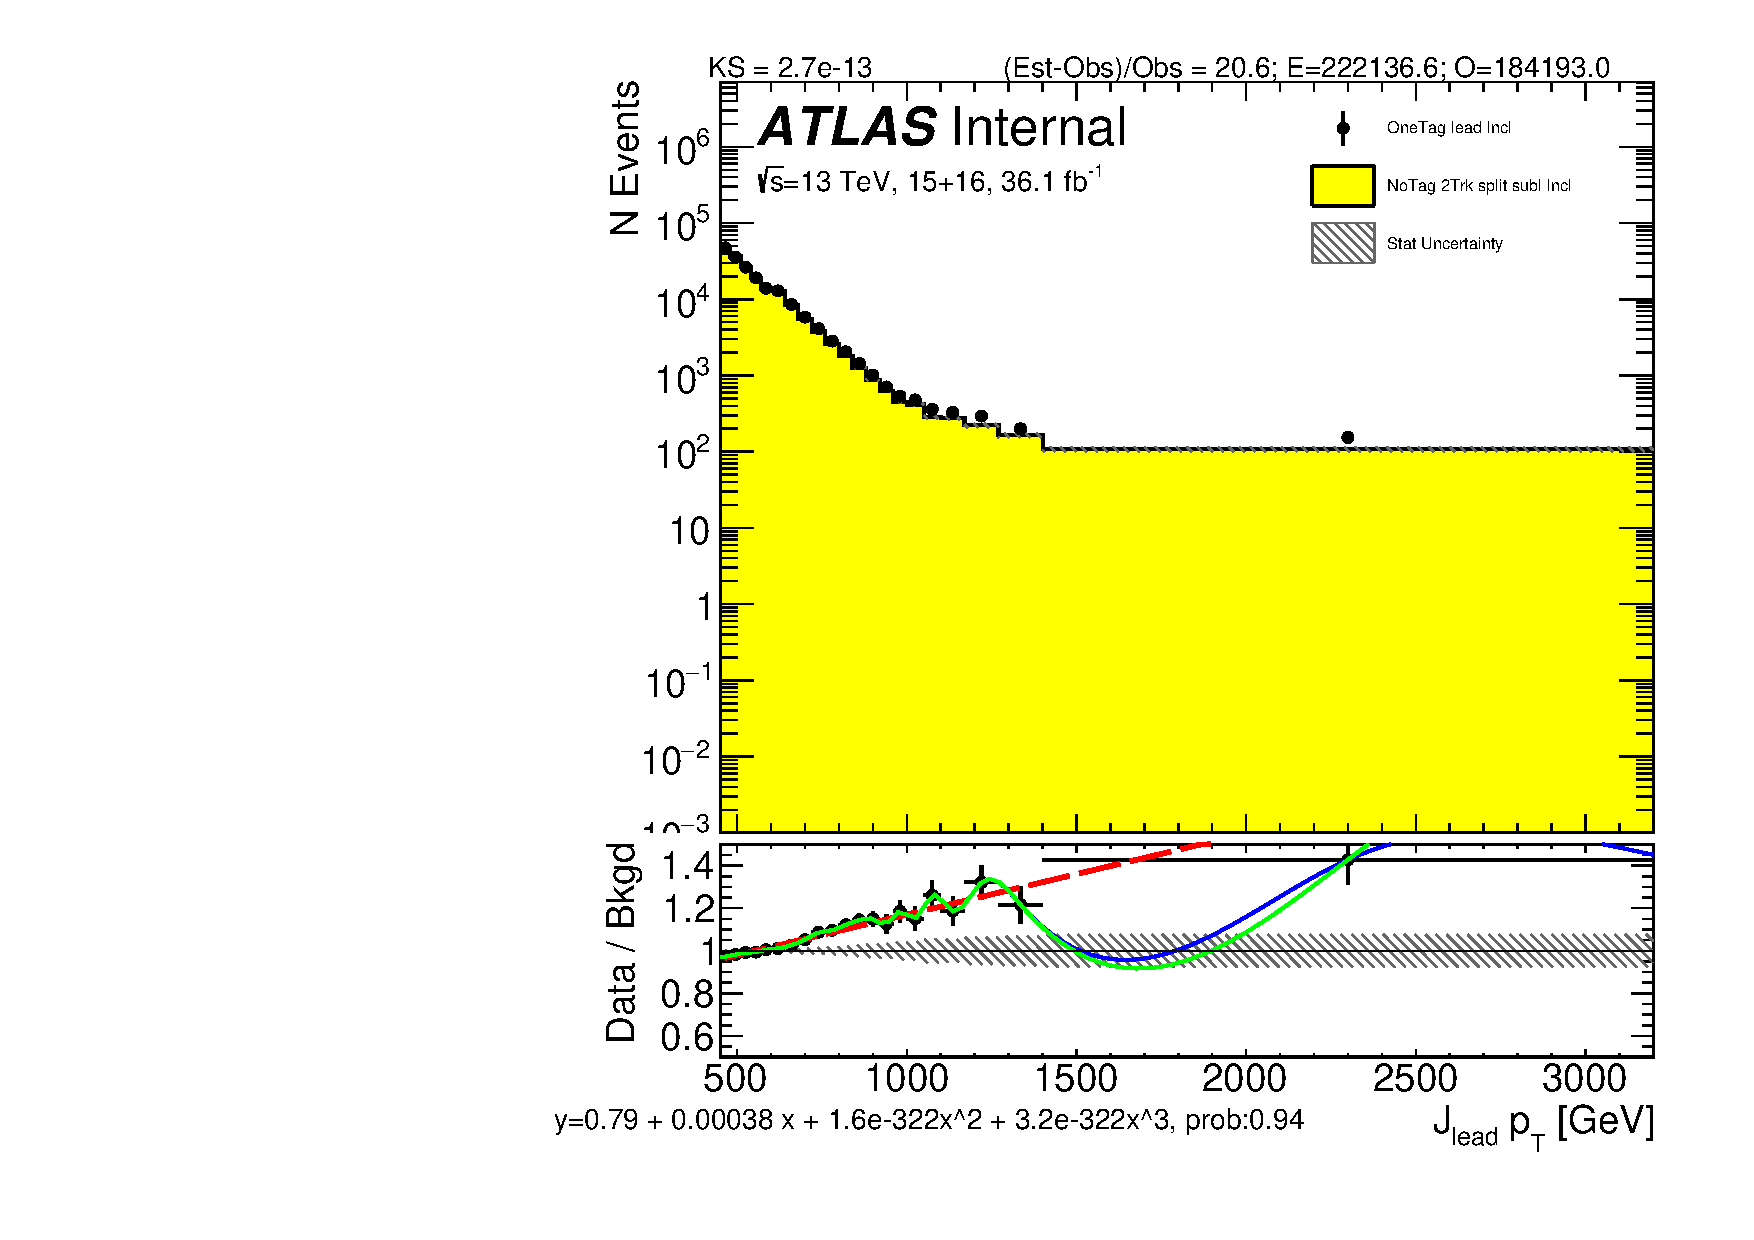
\includegraphics[width=0.25\textwidth,angle=-90]{figures/boosted/Reweight/Fits/Moriond_bkg_0_NoTag_2Trk_split_subl_Incl_leadHCand_Pt_m_1.pdf}
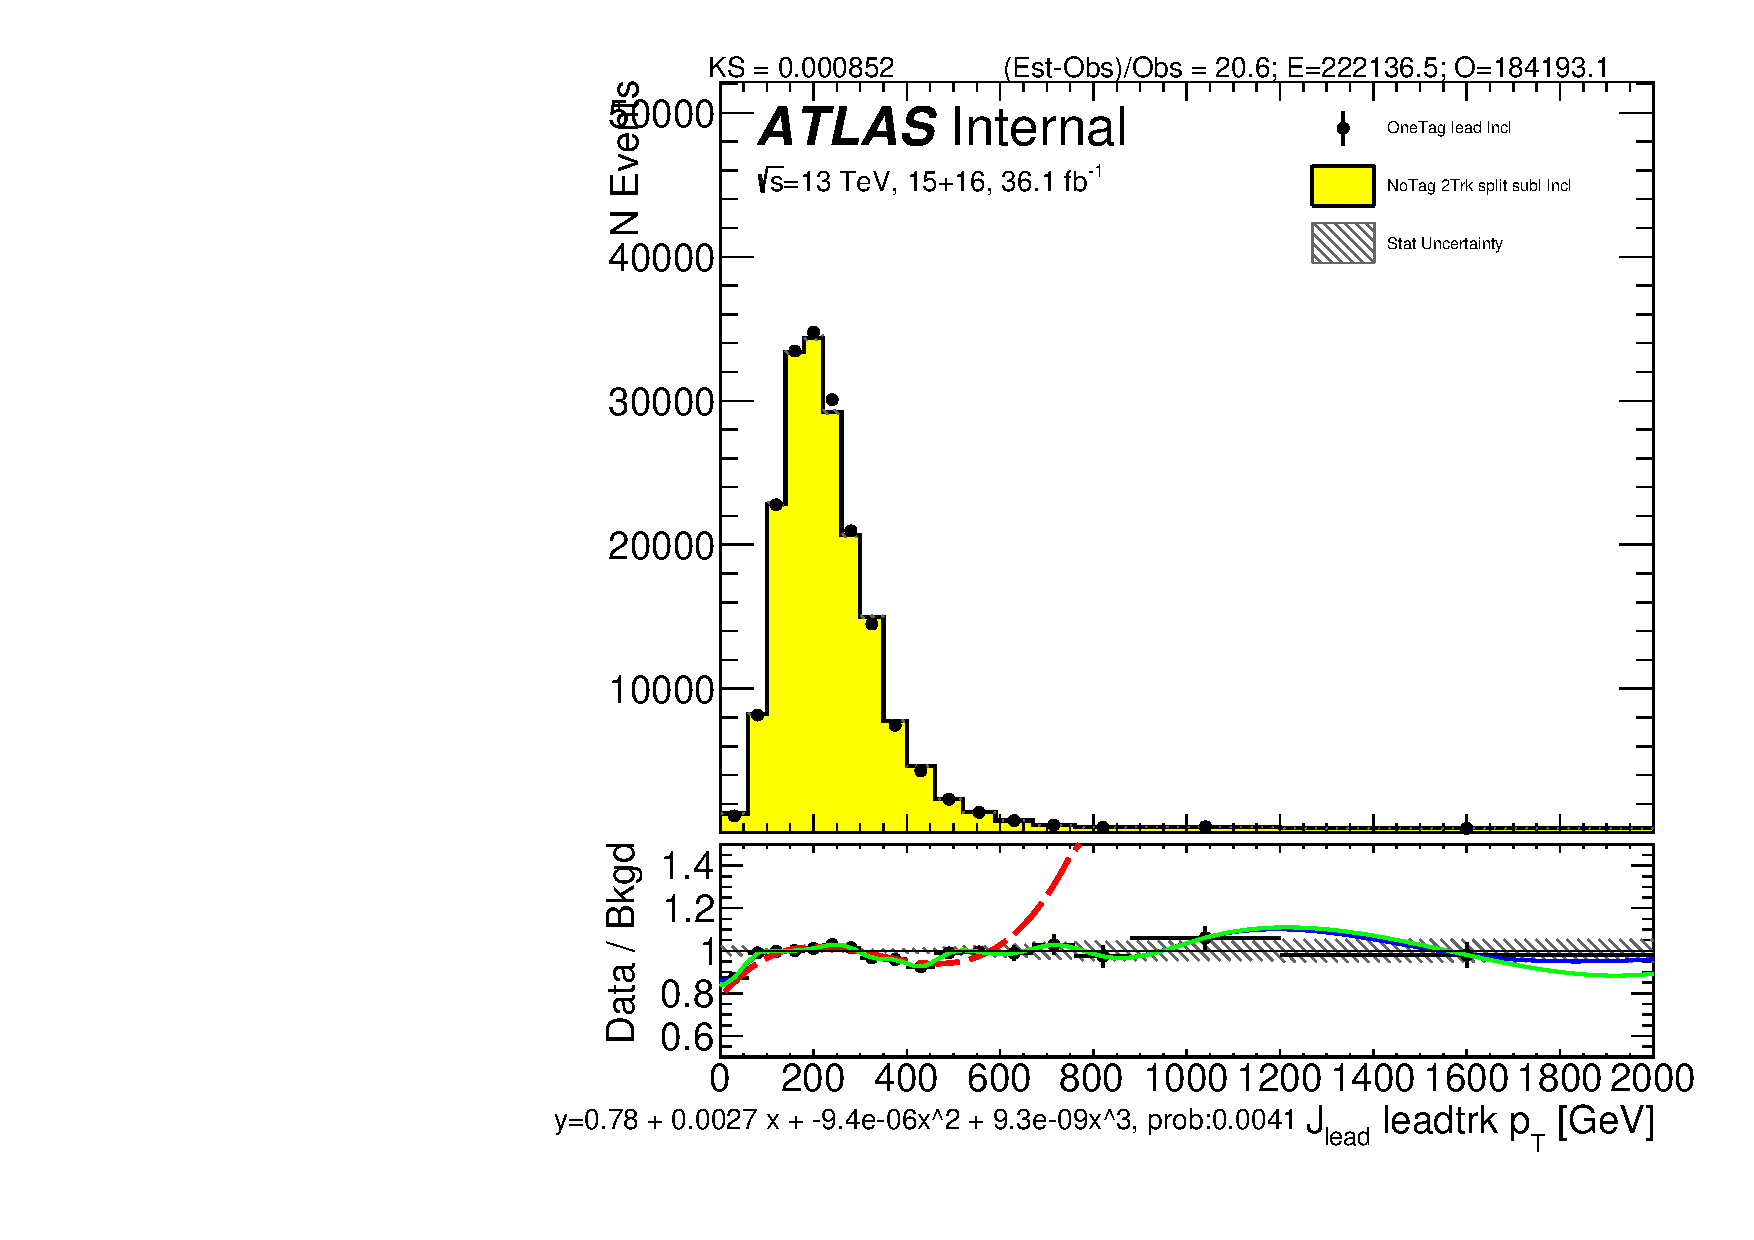
\includegraphics[width=0.25\textwidth,angle=-90]{figures/boosted/Reweight/Fits/Moriond_bkg_0_NoTag_2Trk_split_subl_Incl_leadHCand_trk0_Pt.pdf}
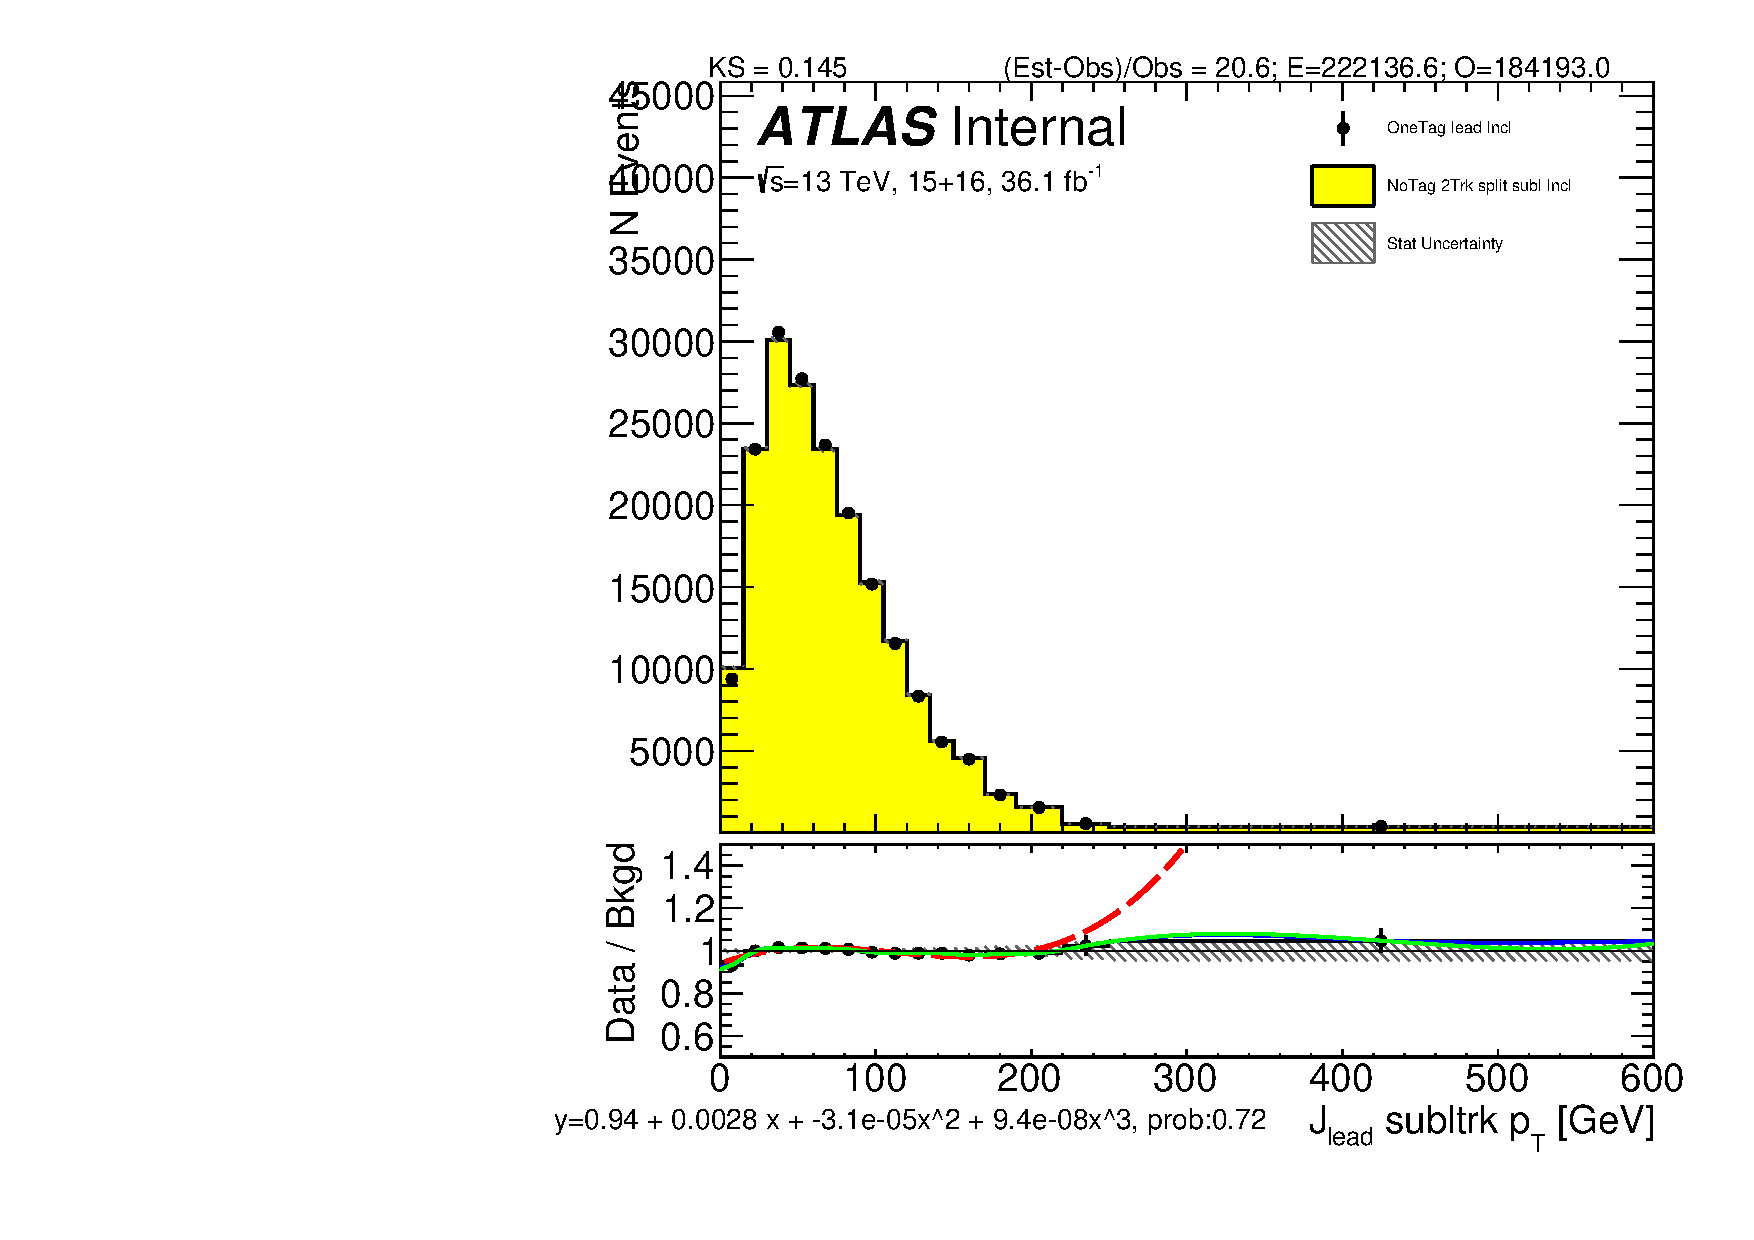
\includegraphics[width=0.25\textwidth,angle=-90]{figures/boosted/Reweight/Fits/Moriond_bkg_0_NoTag_2Trk_split_subl_Incl_leadHCand_trk1_Pt.pdf} \\
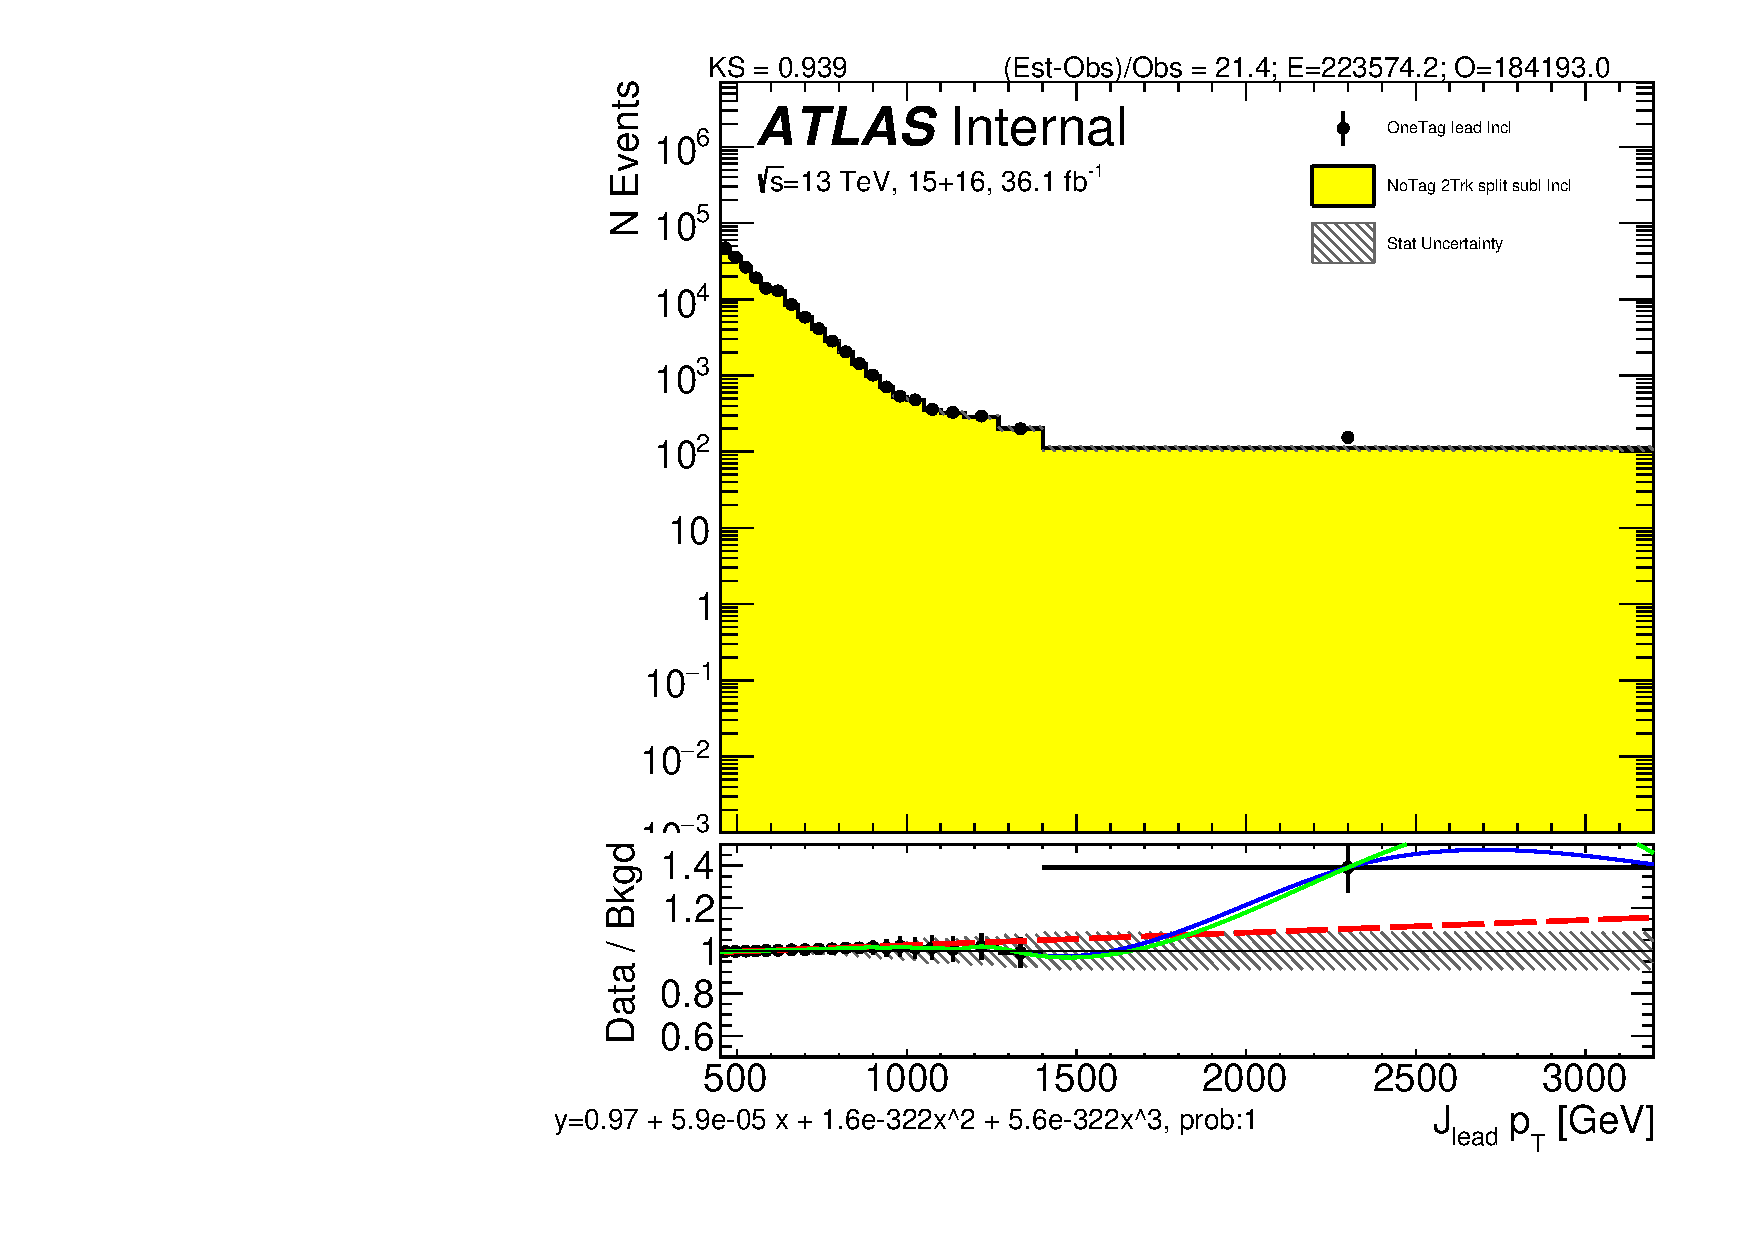
\includegraphics[width=0.25\textwidth,angle=-90]{figures/boosted/Reweight/Fits/Moriond_bkg_3_NoTag_2Trk_split_subl_Incl_leadHCand_Pt_m_1.pdf}
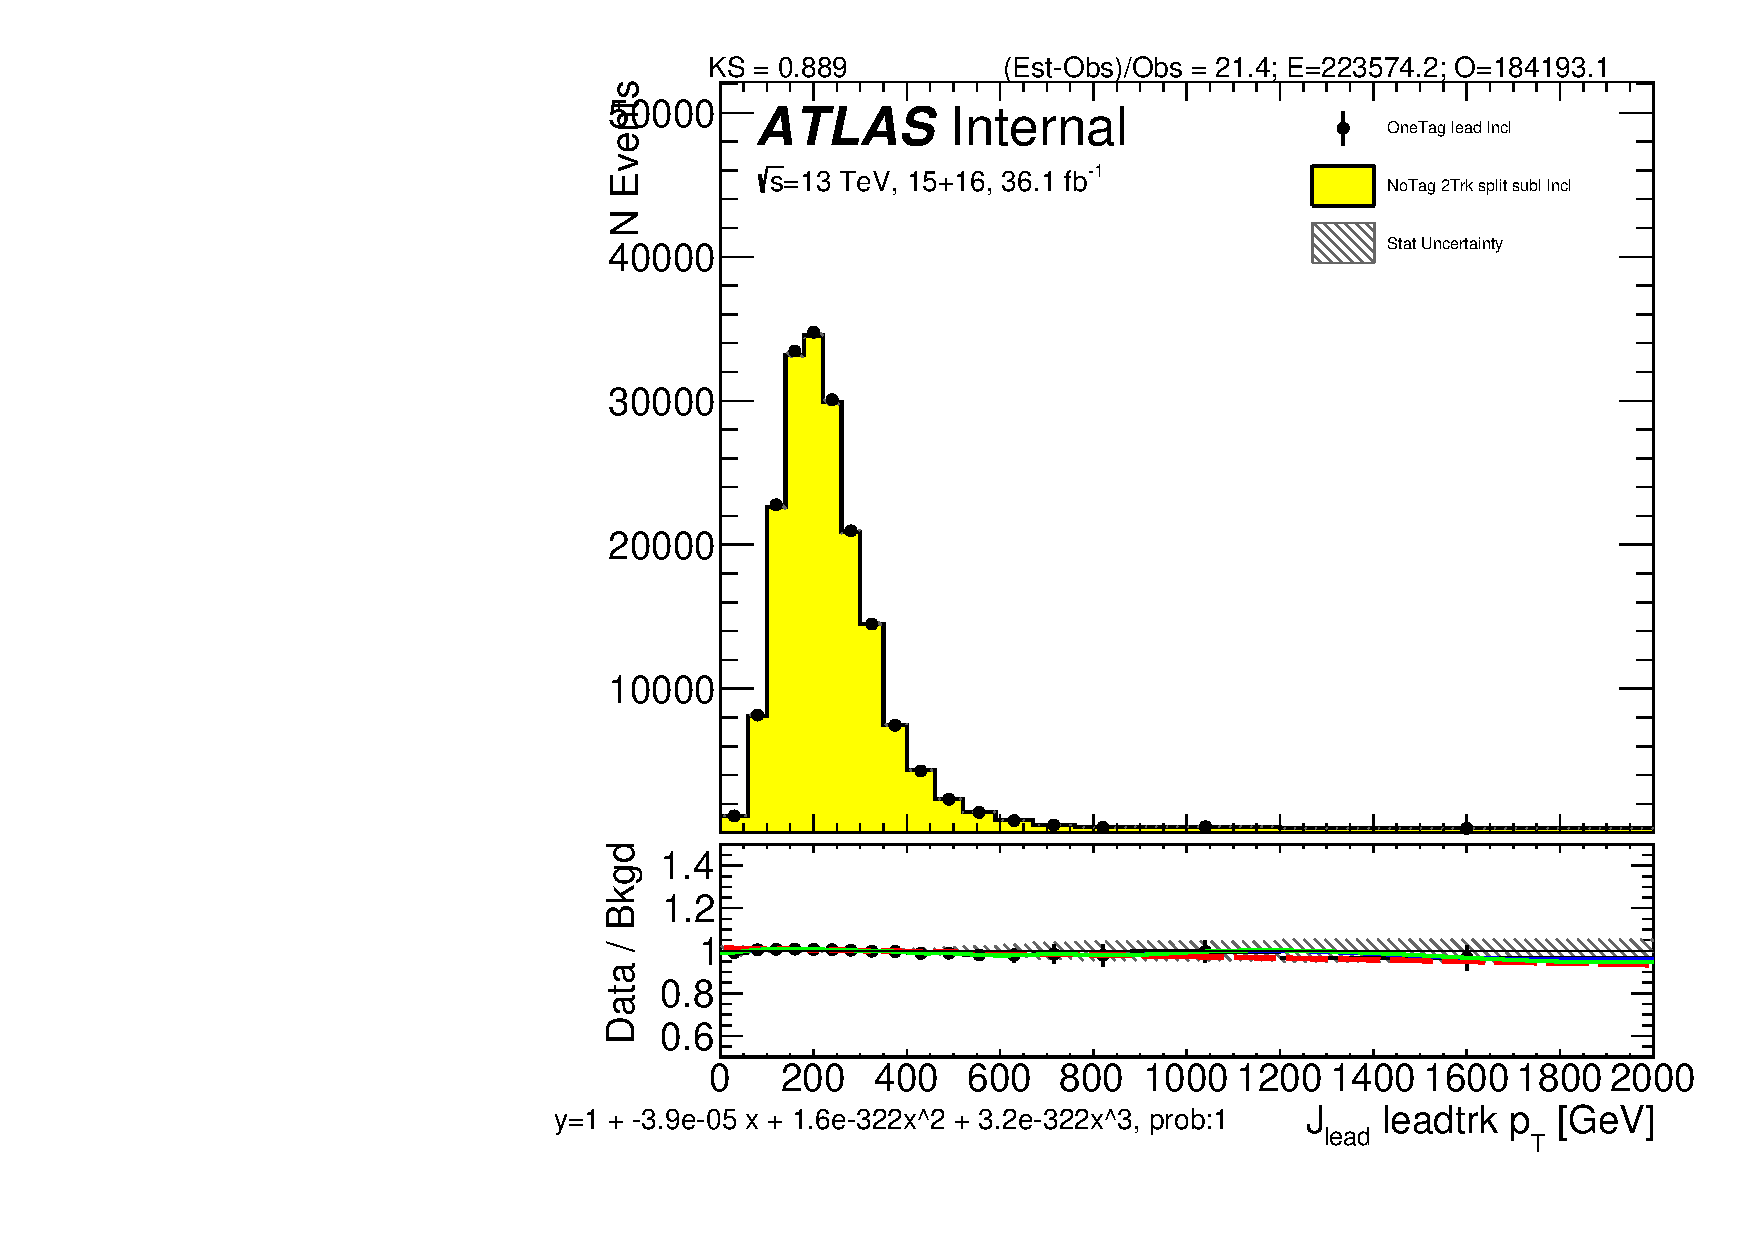
\includegraphics[width=0.25\textwidth,angle=-90]{figures/boosted/Reweight/Fits/Moriond_bkg_3_NoTag_2Trk_split_subl_Incl_leadHCand_trk0_Pt.pdf}
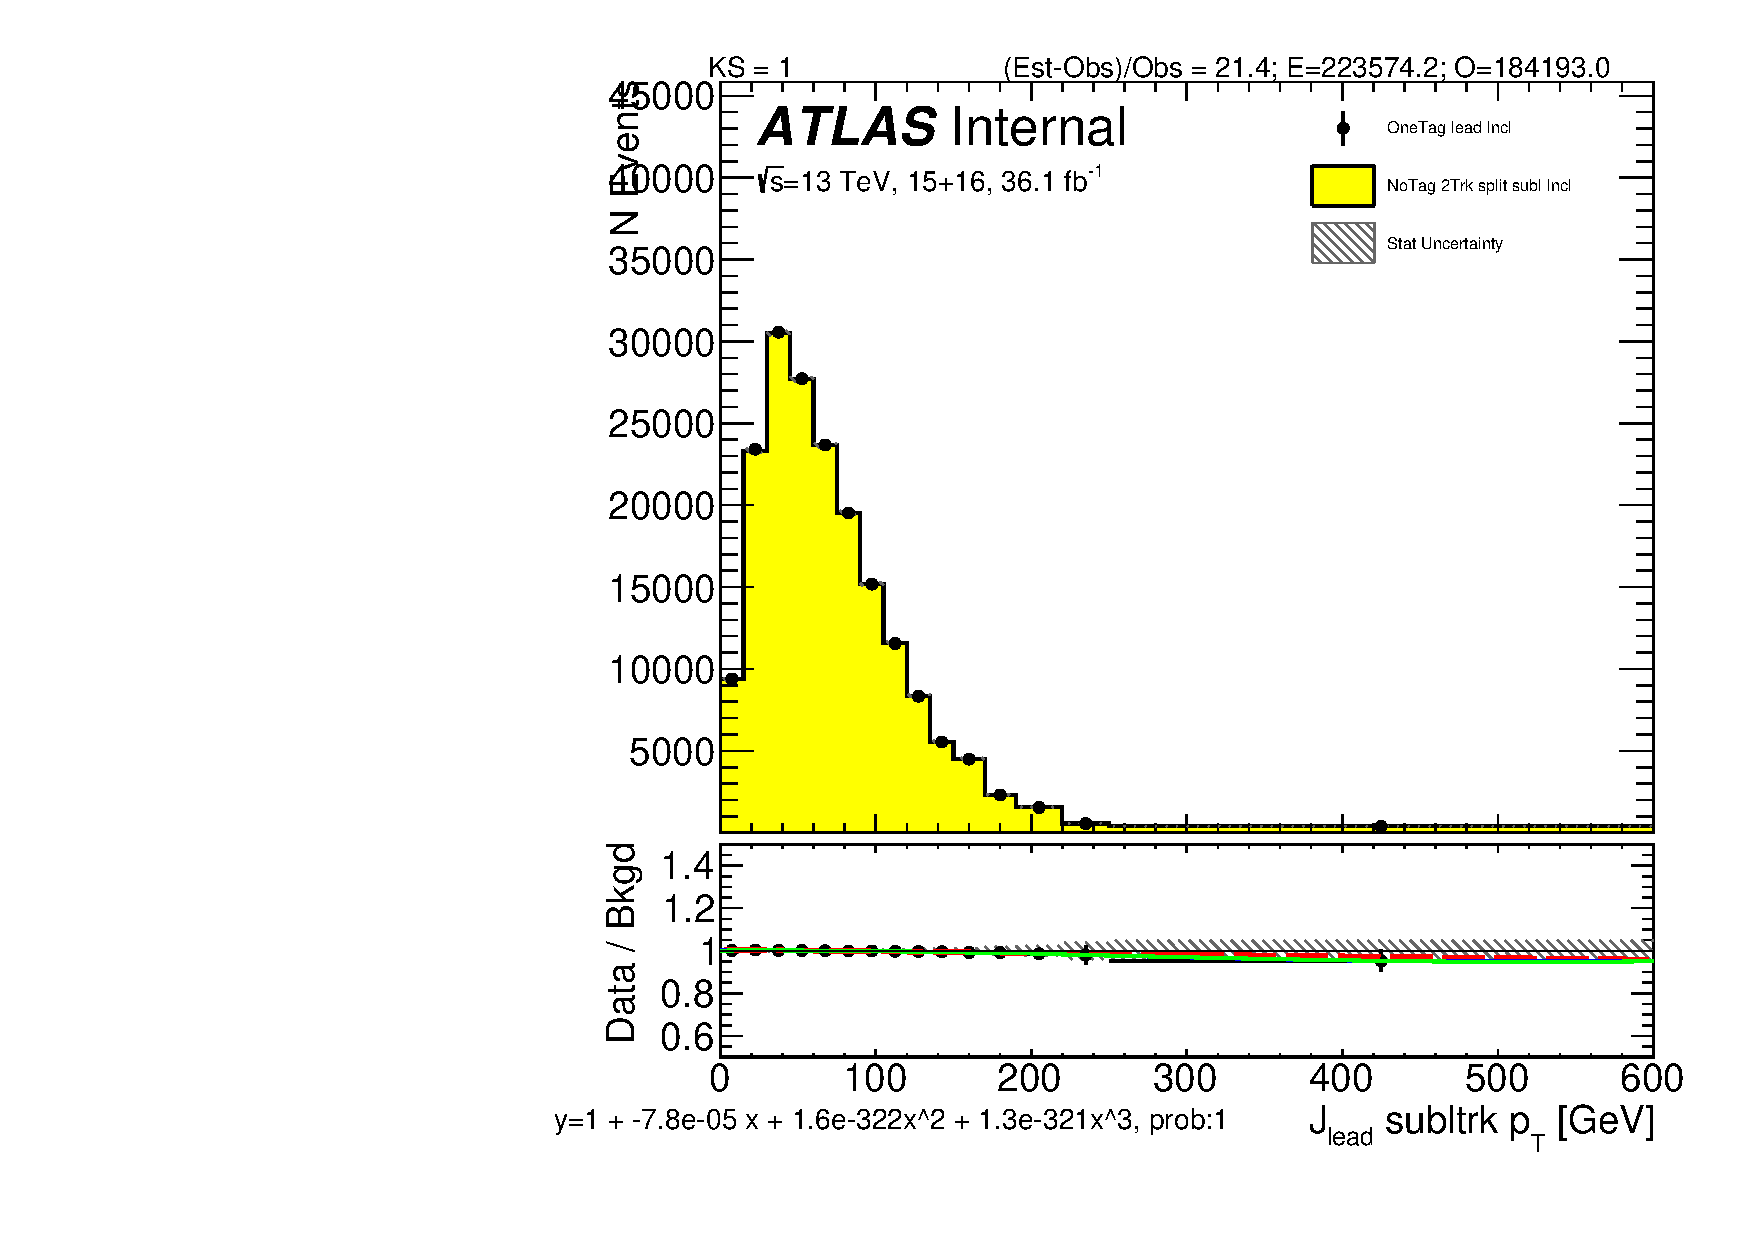
\includegraphics[width=0.25\textwidth,angle=-90]{figures/boosted/Reweight/Fits/Moriond_bkg_3_NoTag_2Trk_split_subl_Incl_leadHCand_trk1_Pt.pdf} \\
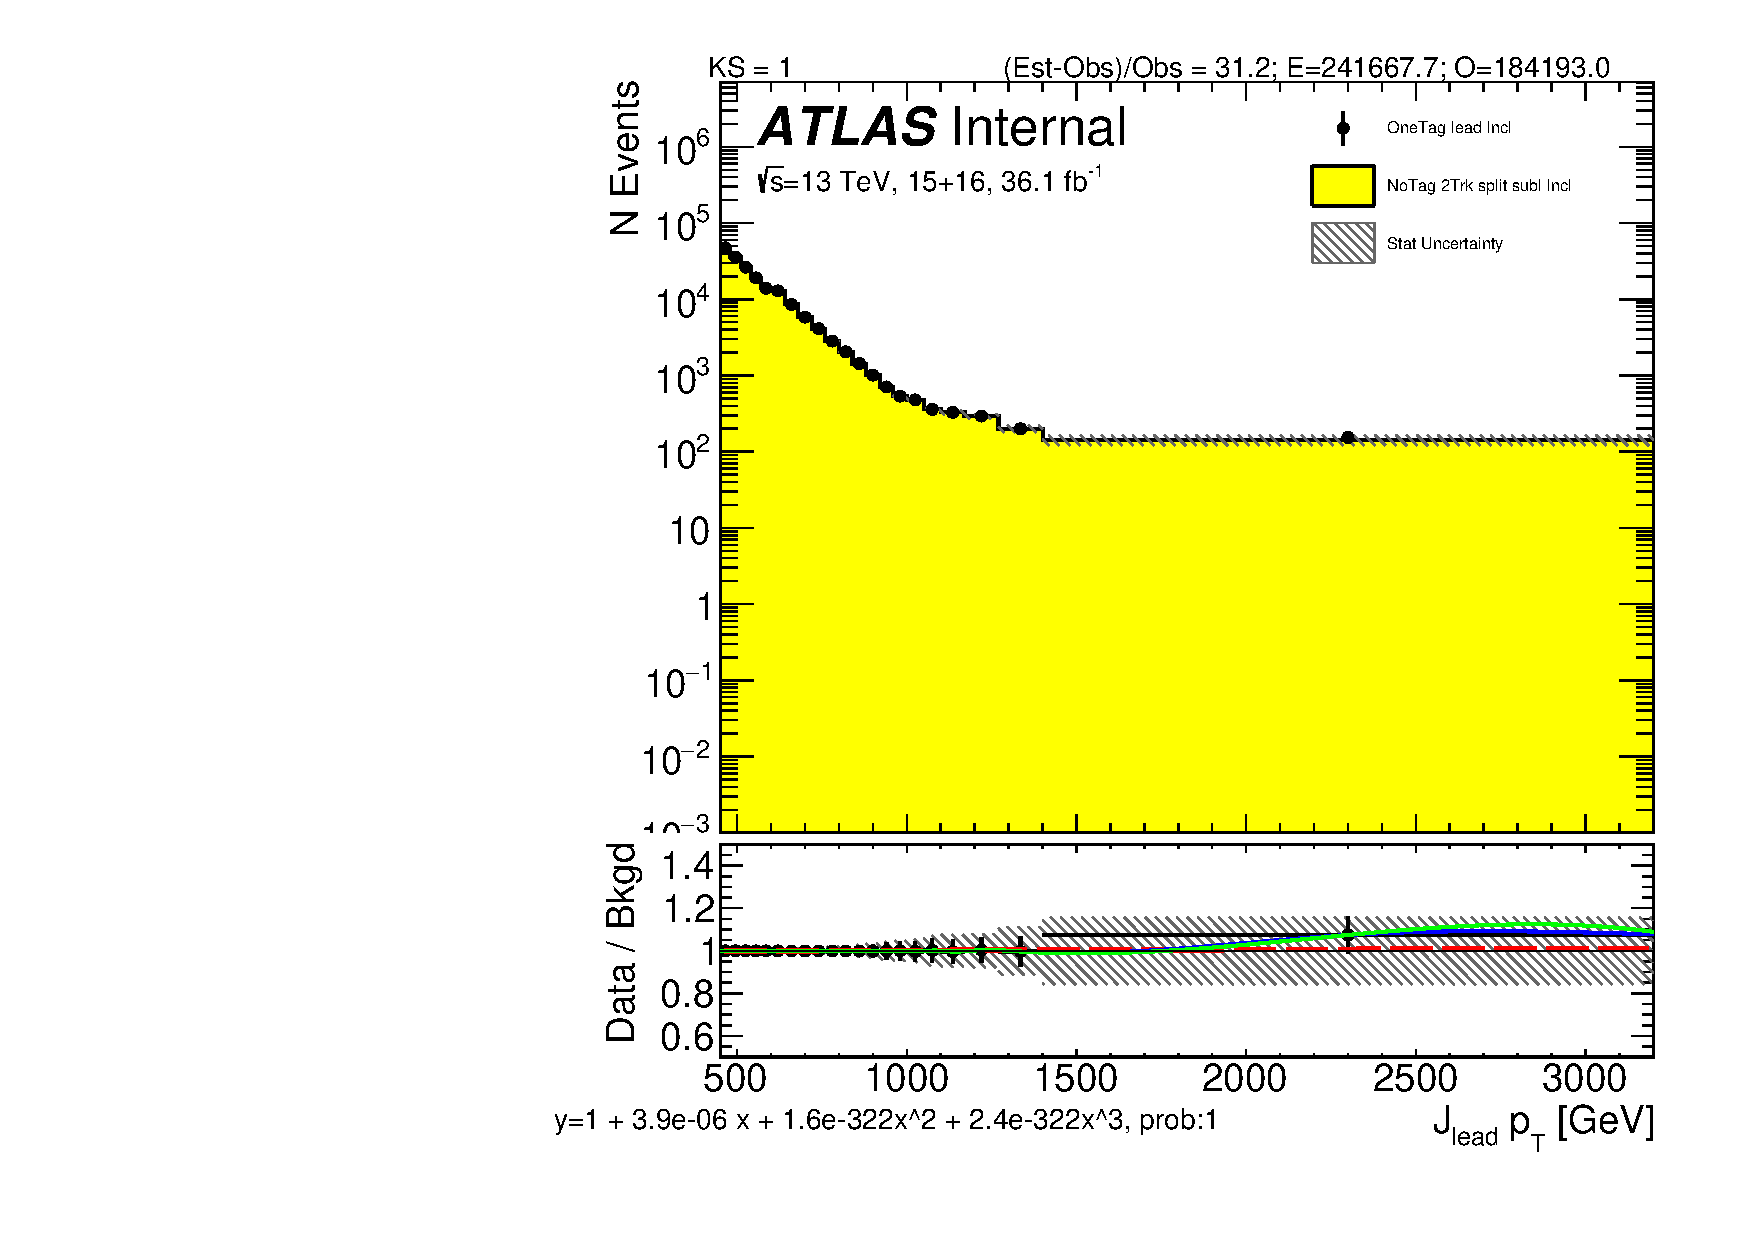
\includegraphics[width=0.25\textwidth,angle=-90]{figures/boosted/Reweight/Fits/Moriond_bkg_9_NoTag_2Trk_split_subl_Incl_leadHCand_Pt_m_1.pdf}
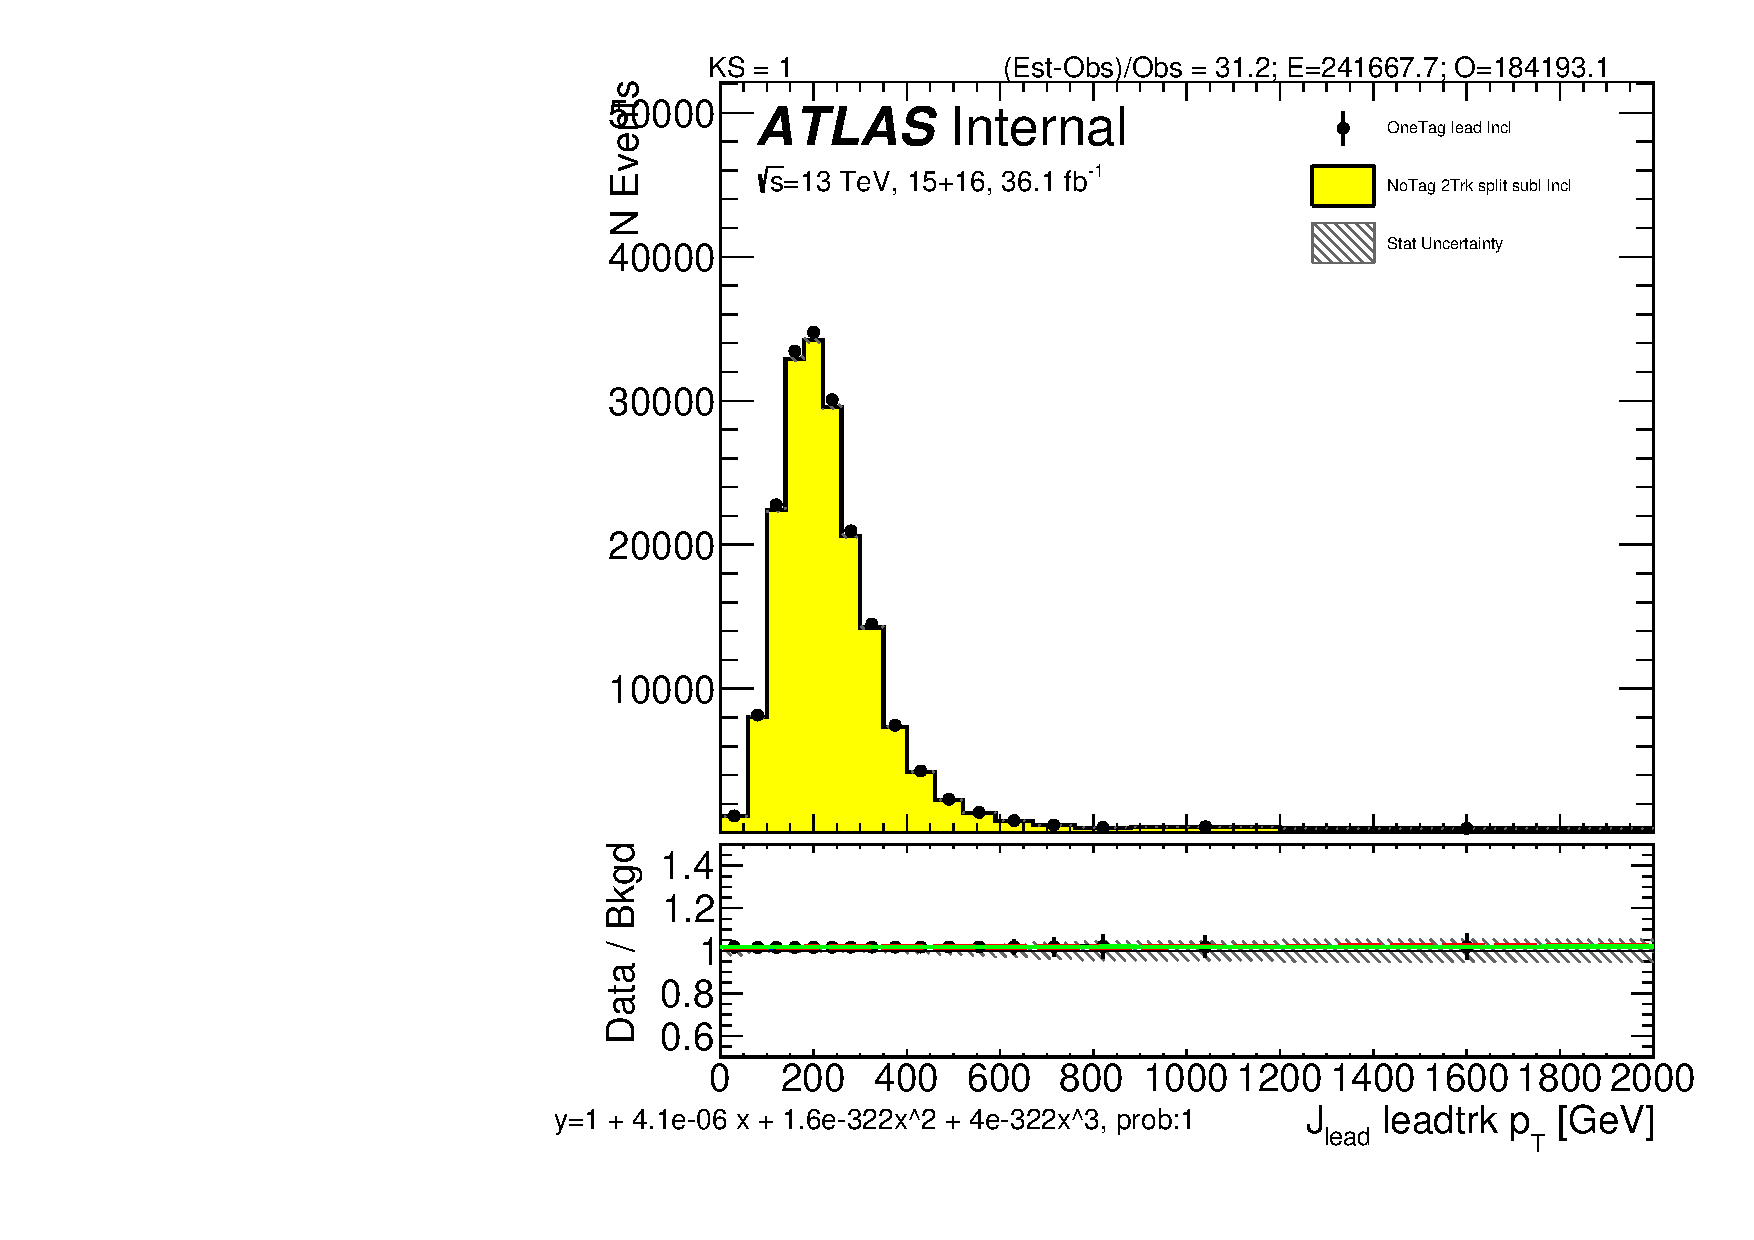
\includegraphics[width=0.25\textwidth,angle=-90]{figures/boosted/Reweight/Fits/Moriond_bkg_9_NoTag_2Trk_split_subl_Incl_leadHCand_trk0_Pt.pdf}
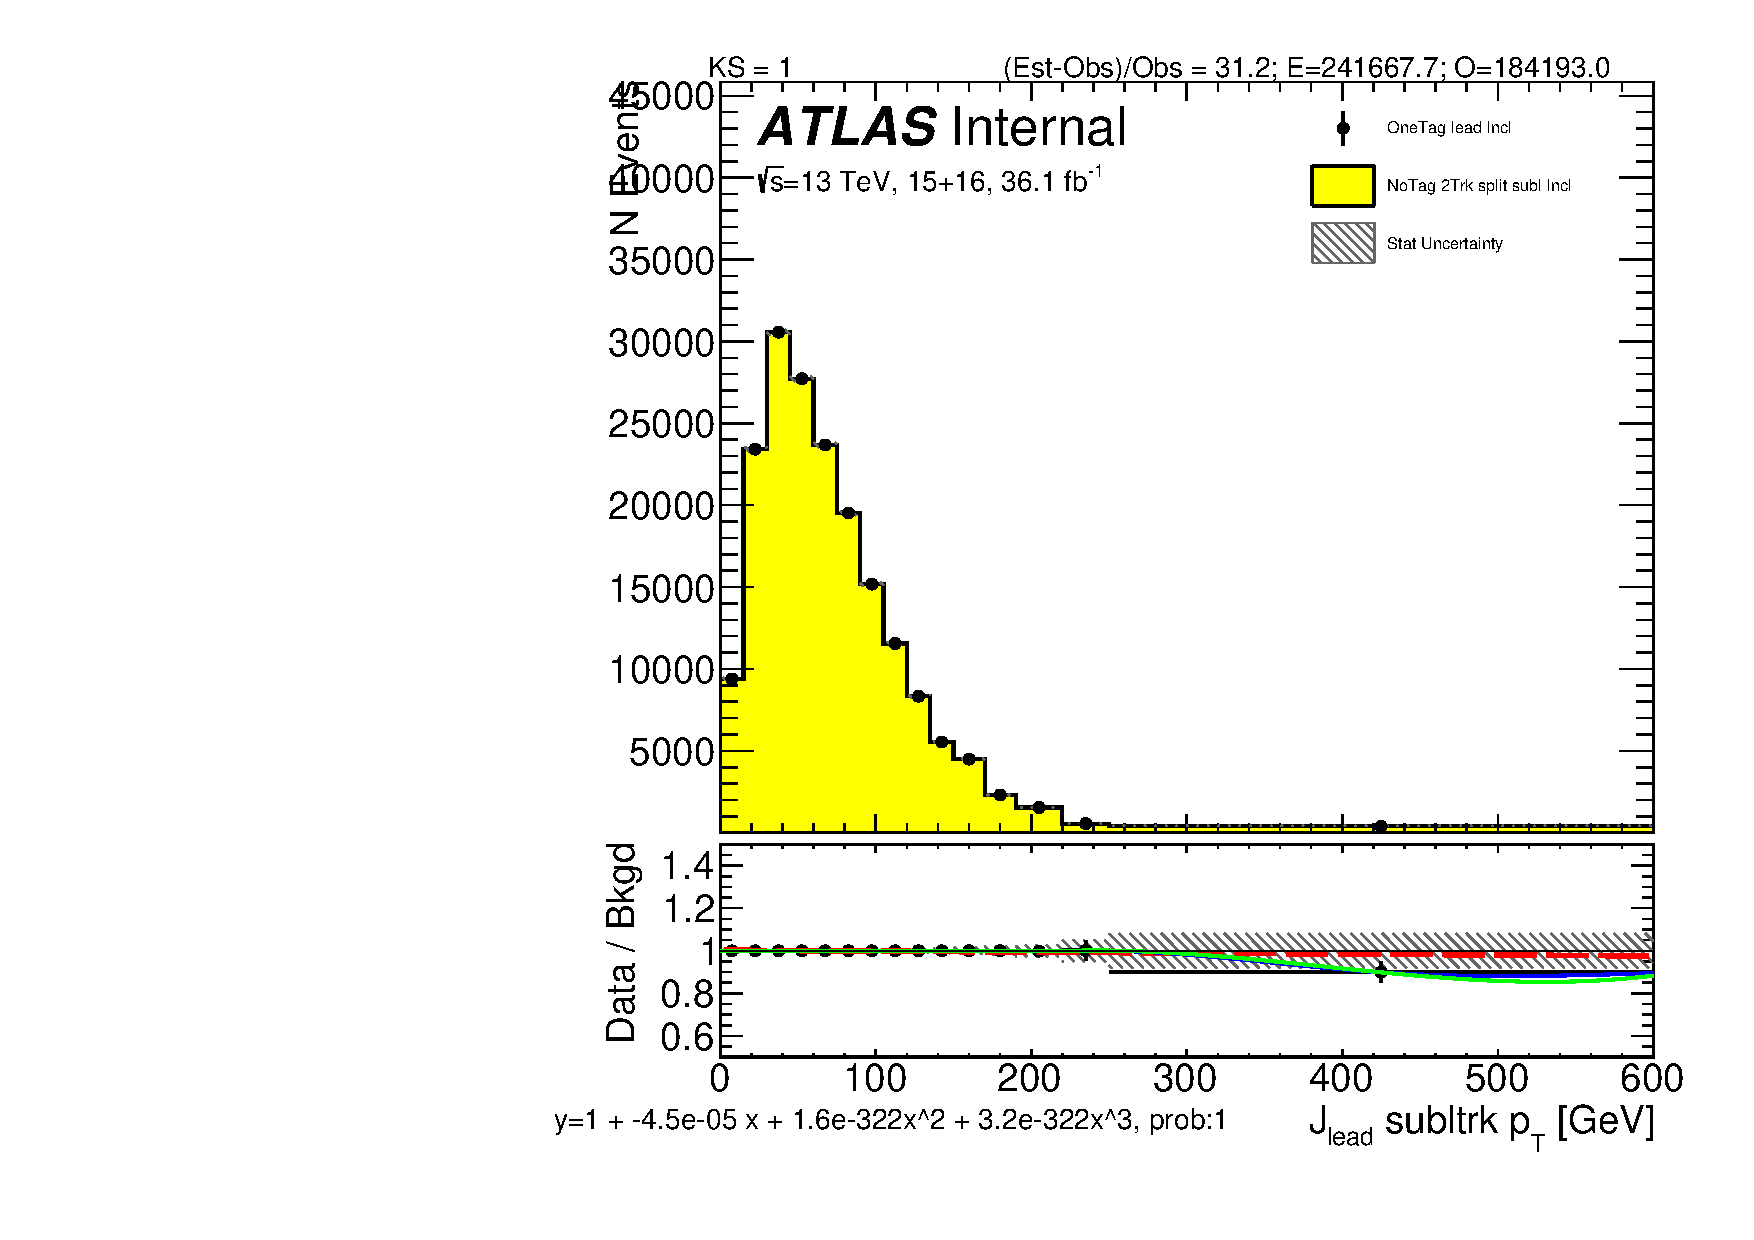
\includegraphics[width=0.25\textwidth,angle=-90]{figures/boosted/Reweight/Fits/Moriond_bkg_9_NoTag_2Trk_split_subl_Incl_leadHCand_trk1_Pt.pdf} \\
\caption{For $2bs$ background estimate: the fits to the ratio of the data in the $1b$ category, of the leading Higgs candidate $1b$-tagged events's leading Higgs candidate distributions(black point), over the subleading Higgs candidate $1b$-tagged events's leading Higgs candidate distributions(yellow). Distributions and fits to the estimated QCD background for large-\R jet $p_{T}$ (left),  the large-\R jet's leading trackjet $p_T$ (middle), and large-\R jet's subleading trackjet $p_T$ (right) are shown.  Figures are before reweighting (top row), after the first iteration(second row), after the fourth iteration(third row), and after the last iteration (bottom row). The green line is the spline fit; the red line is a polynomial fit; the blue line is the spline interpolation.}
\label{fig:rw-2bs-subl}
\end{center}
\end{figure*}

\begin{figure*}[htbp!]
\begin{center}
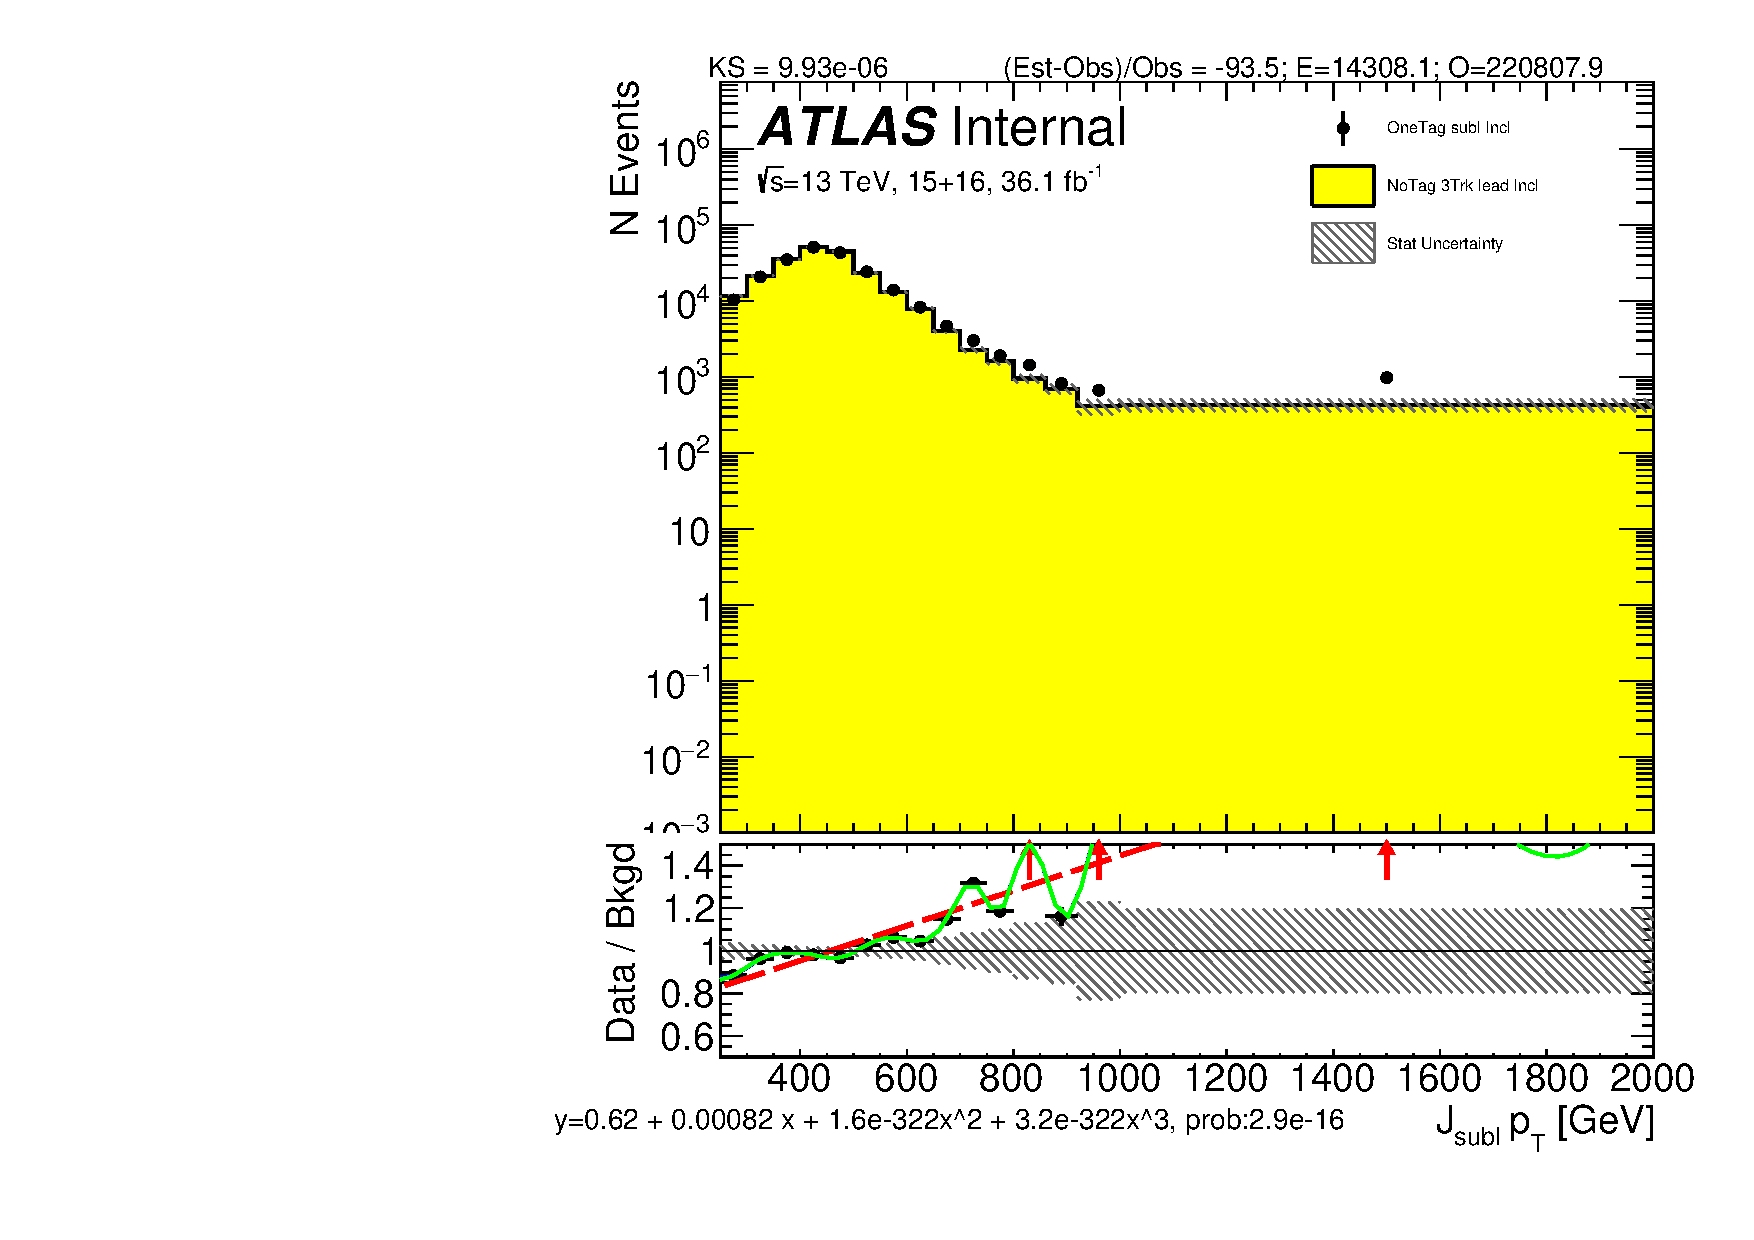
\includegraphics[width=0.25\textwidth,angle=-90]{figures/boosted/Reweight/Fits/Moriond_NoTag_3Trk_lead_Incl_sublHCand_Pt_m_1.pdf}
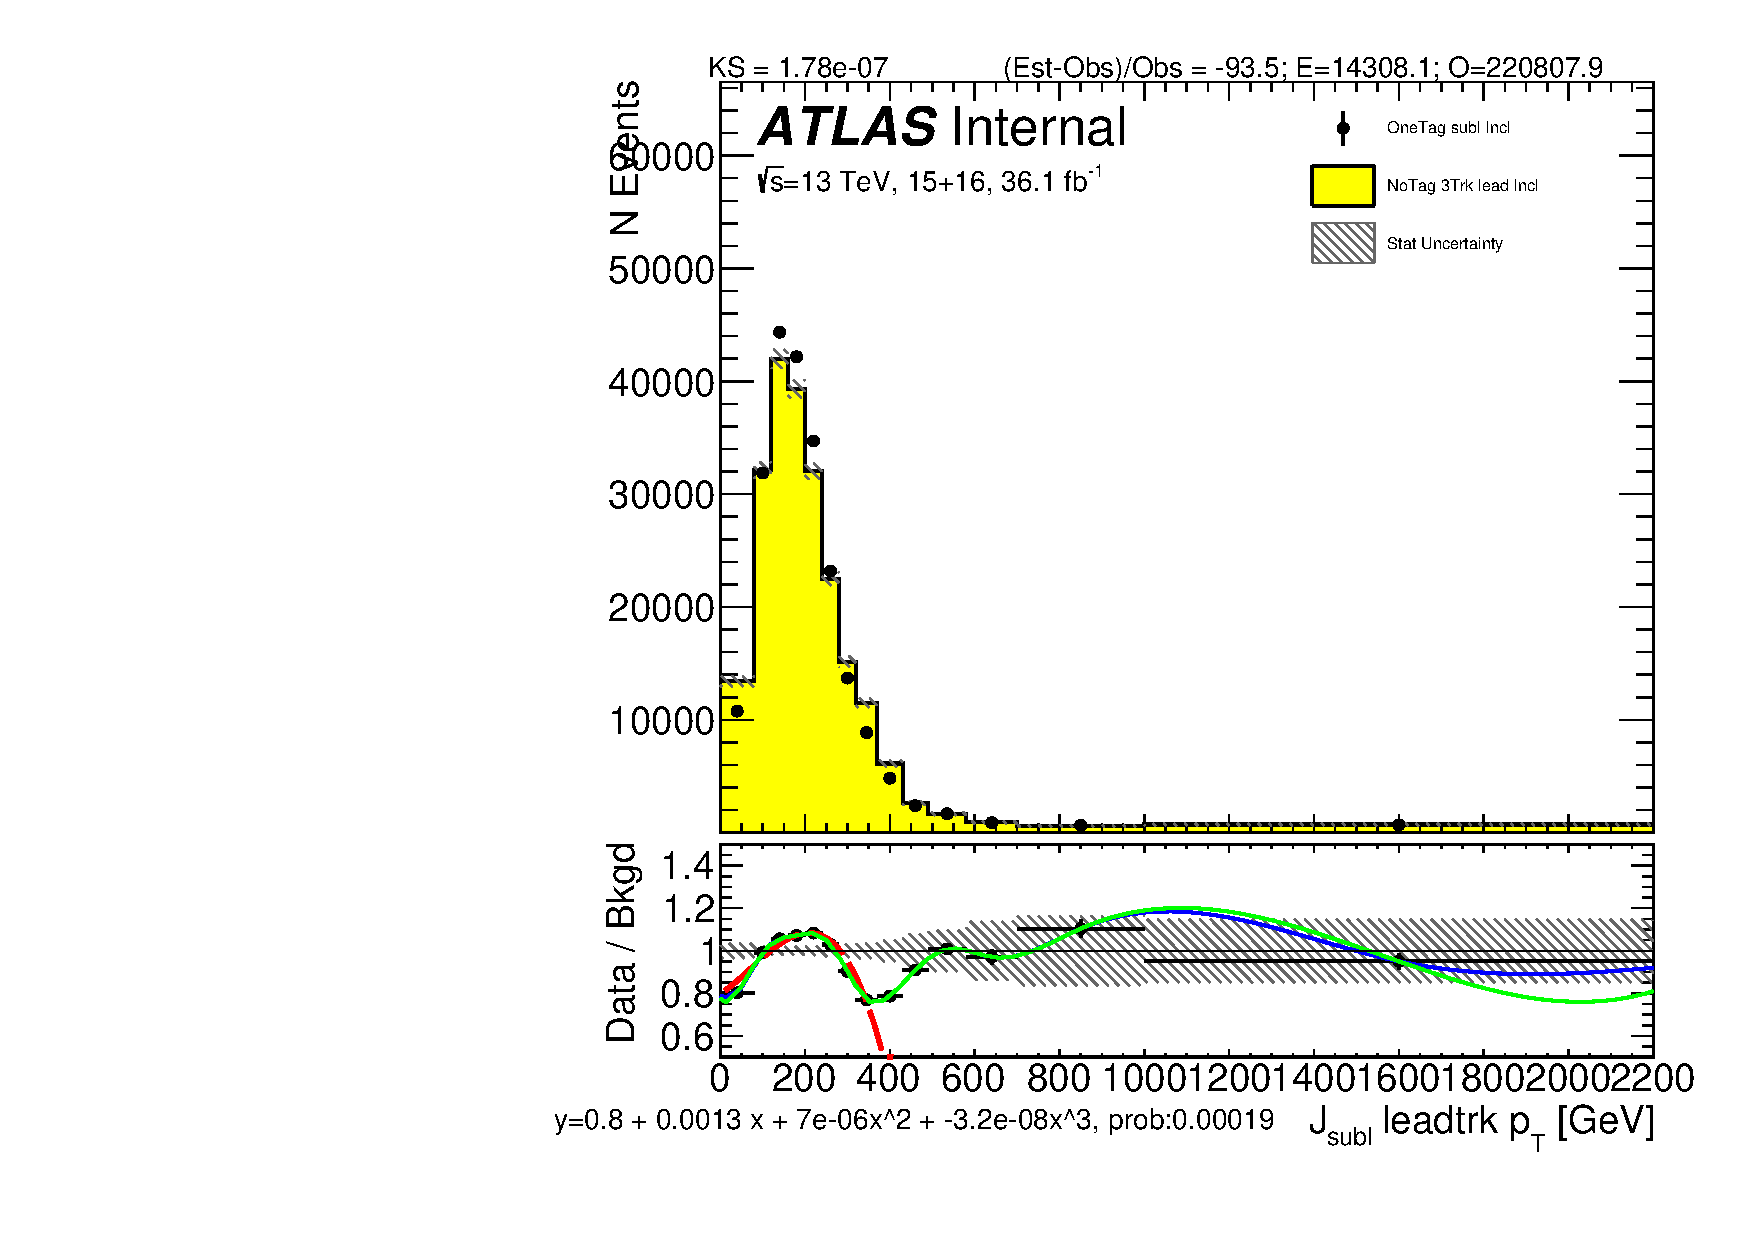
\includegraphics[width=0.25\textwidth,angle=-90]{figures/boosted/Reweight/Fits/Moriond_NoTag_3Trk_lead_Incl_sublHCand_trk0_Pt.pdf}
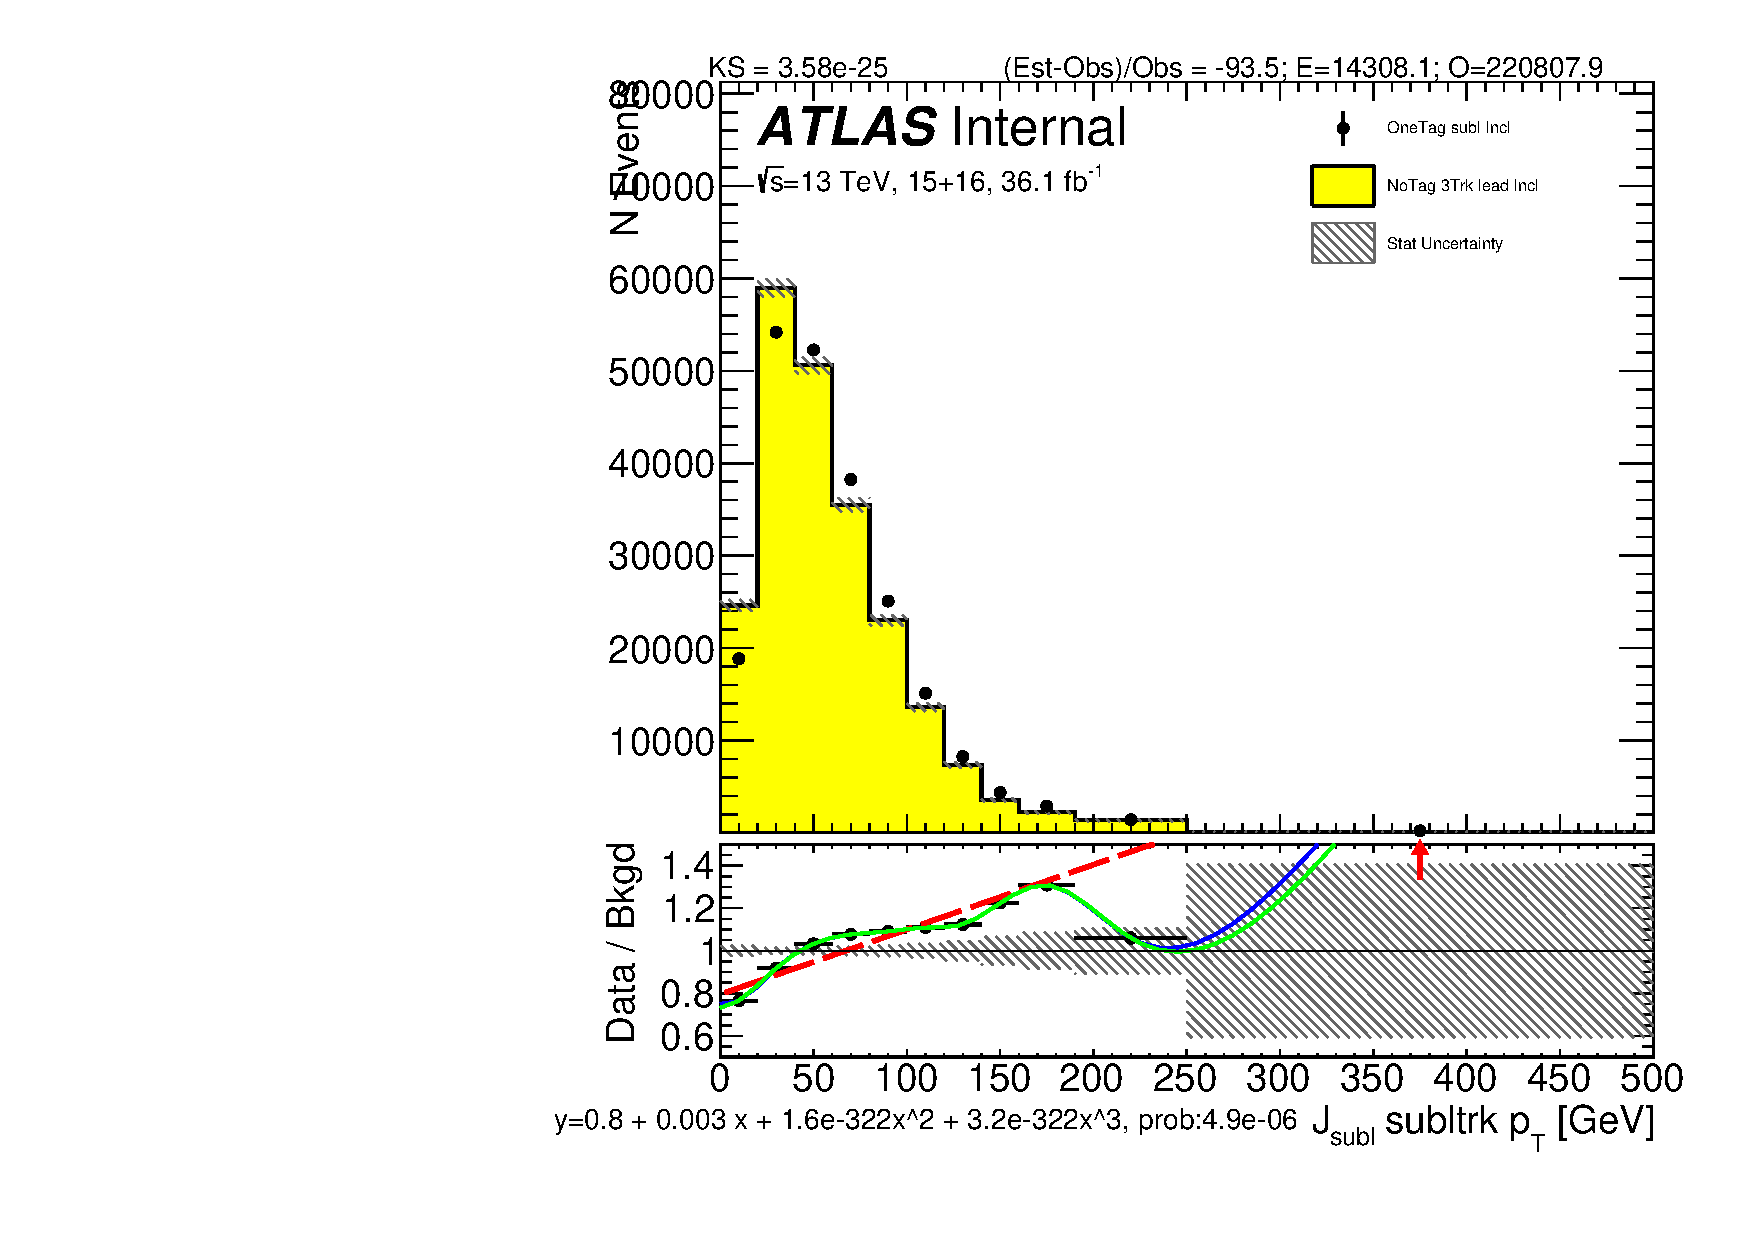
\includegraphics[width=0.25\textwidth,angle=-90]{figures/boosted/Reweight/Fits/Moriond_NoTag_3Trk_lead_Incl_sublHCand_trk1_Pt.pdf} \\
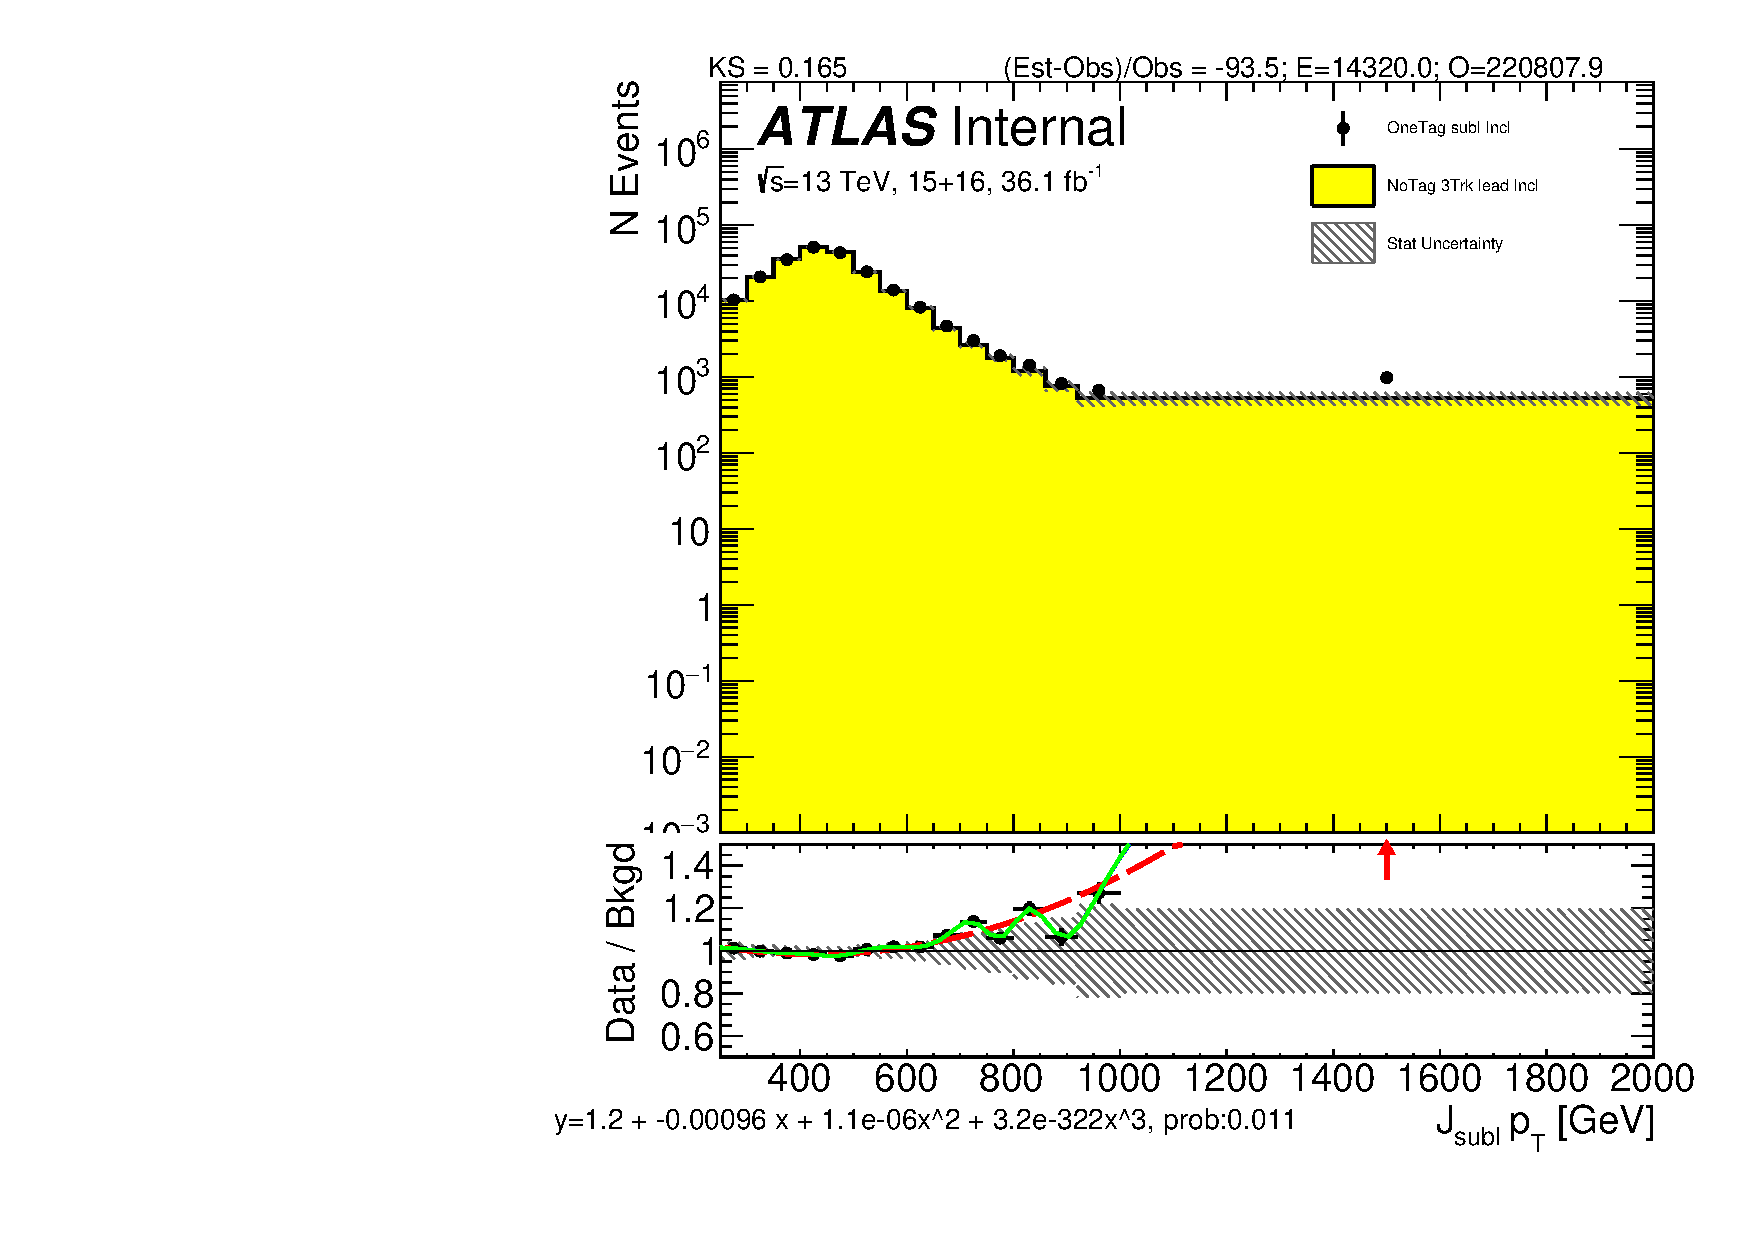
\includegraphics[width=0.25\textwidth,angle=-90]{figures/boosted/Reweight/Fits/Moriond_bkg_0_NoTag_3Trk_lead_Incl_sublHCand_Pt_m_1.pdf}
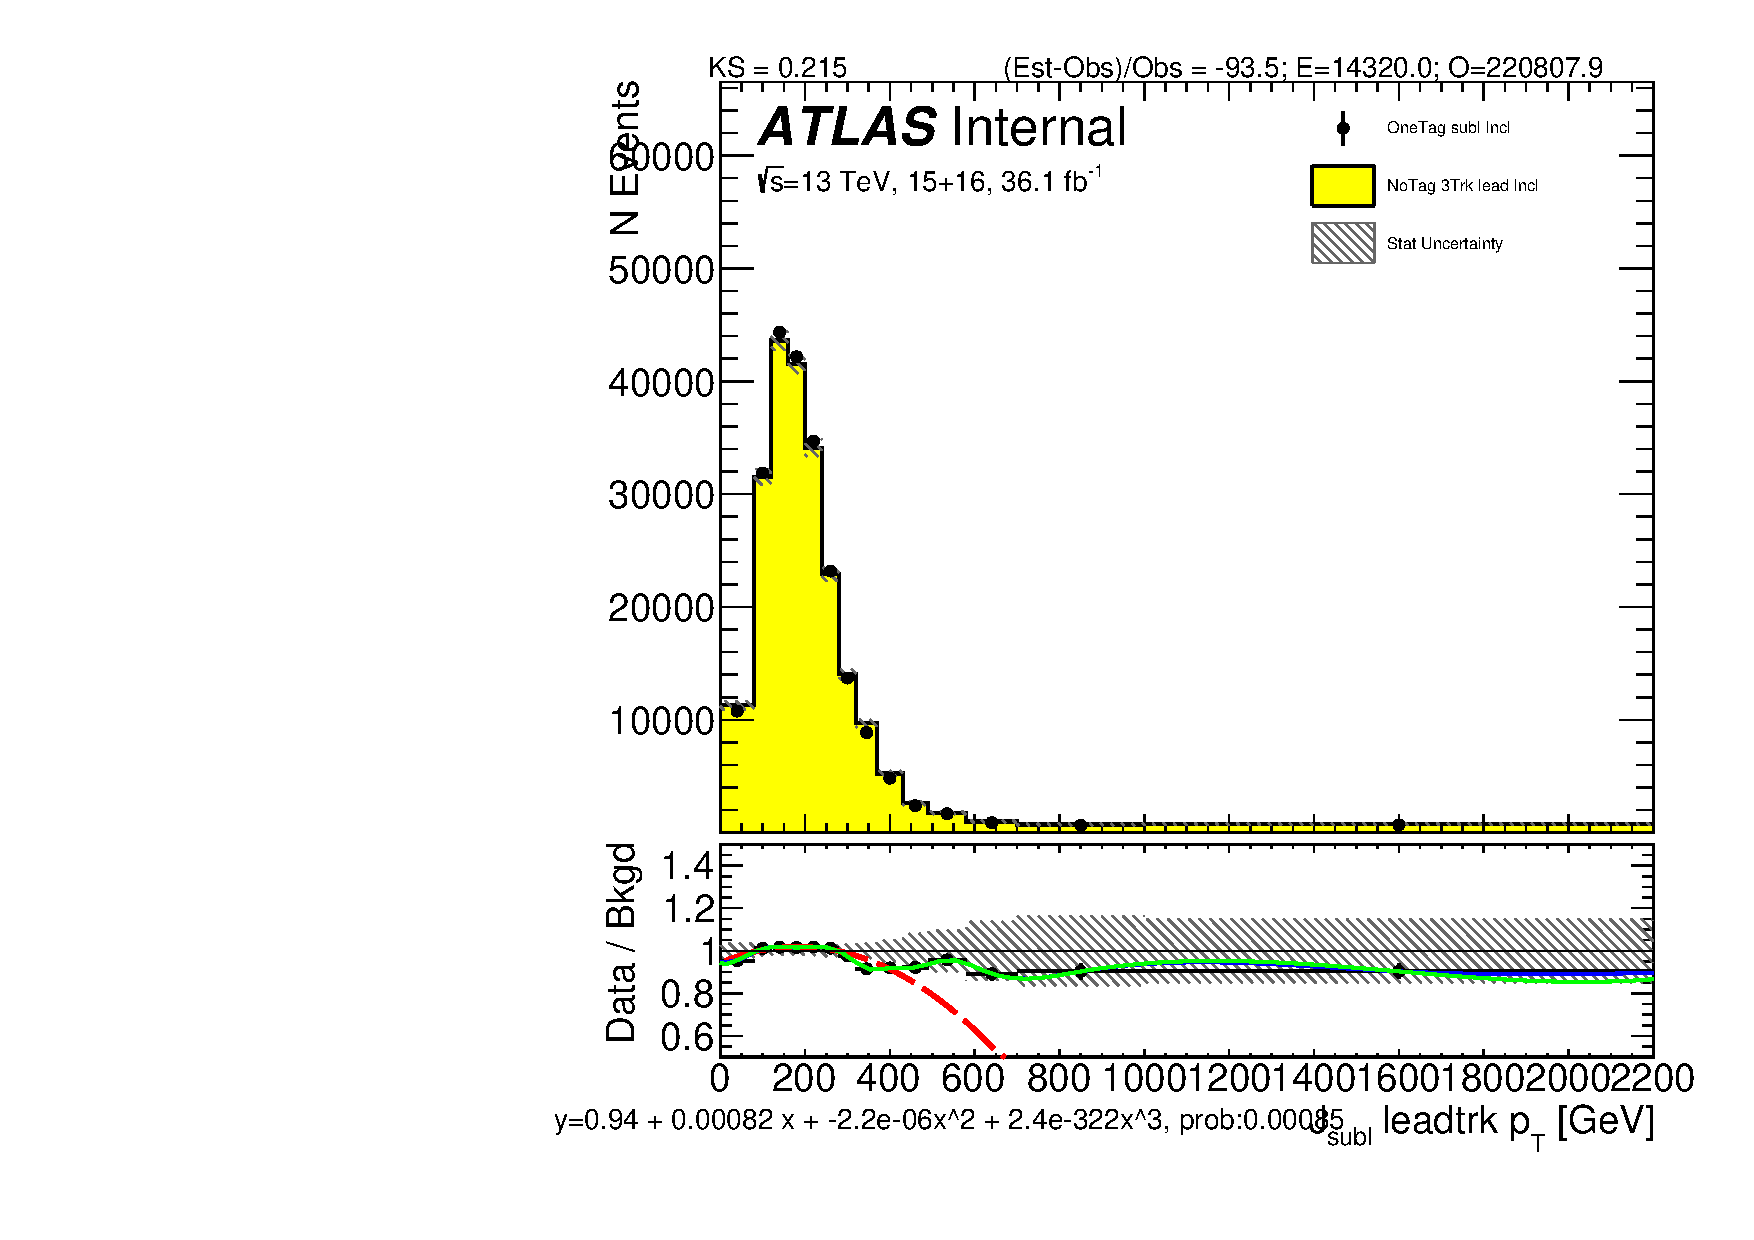
\includegraphics[width=0.25\textwidth,angle=-90]{figures/boosted/Reweight/Fits/Moriond_bkg_0_NoTag_3Trk_lead_Incl_sublHCand_trk0_Pt.pdf}
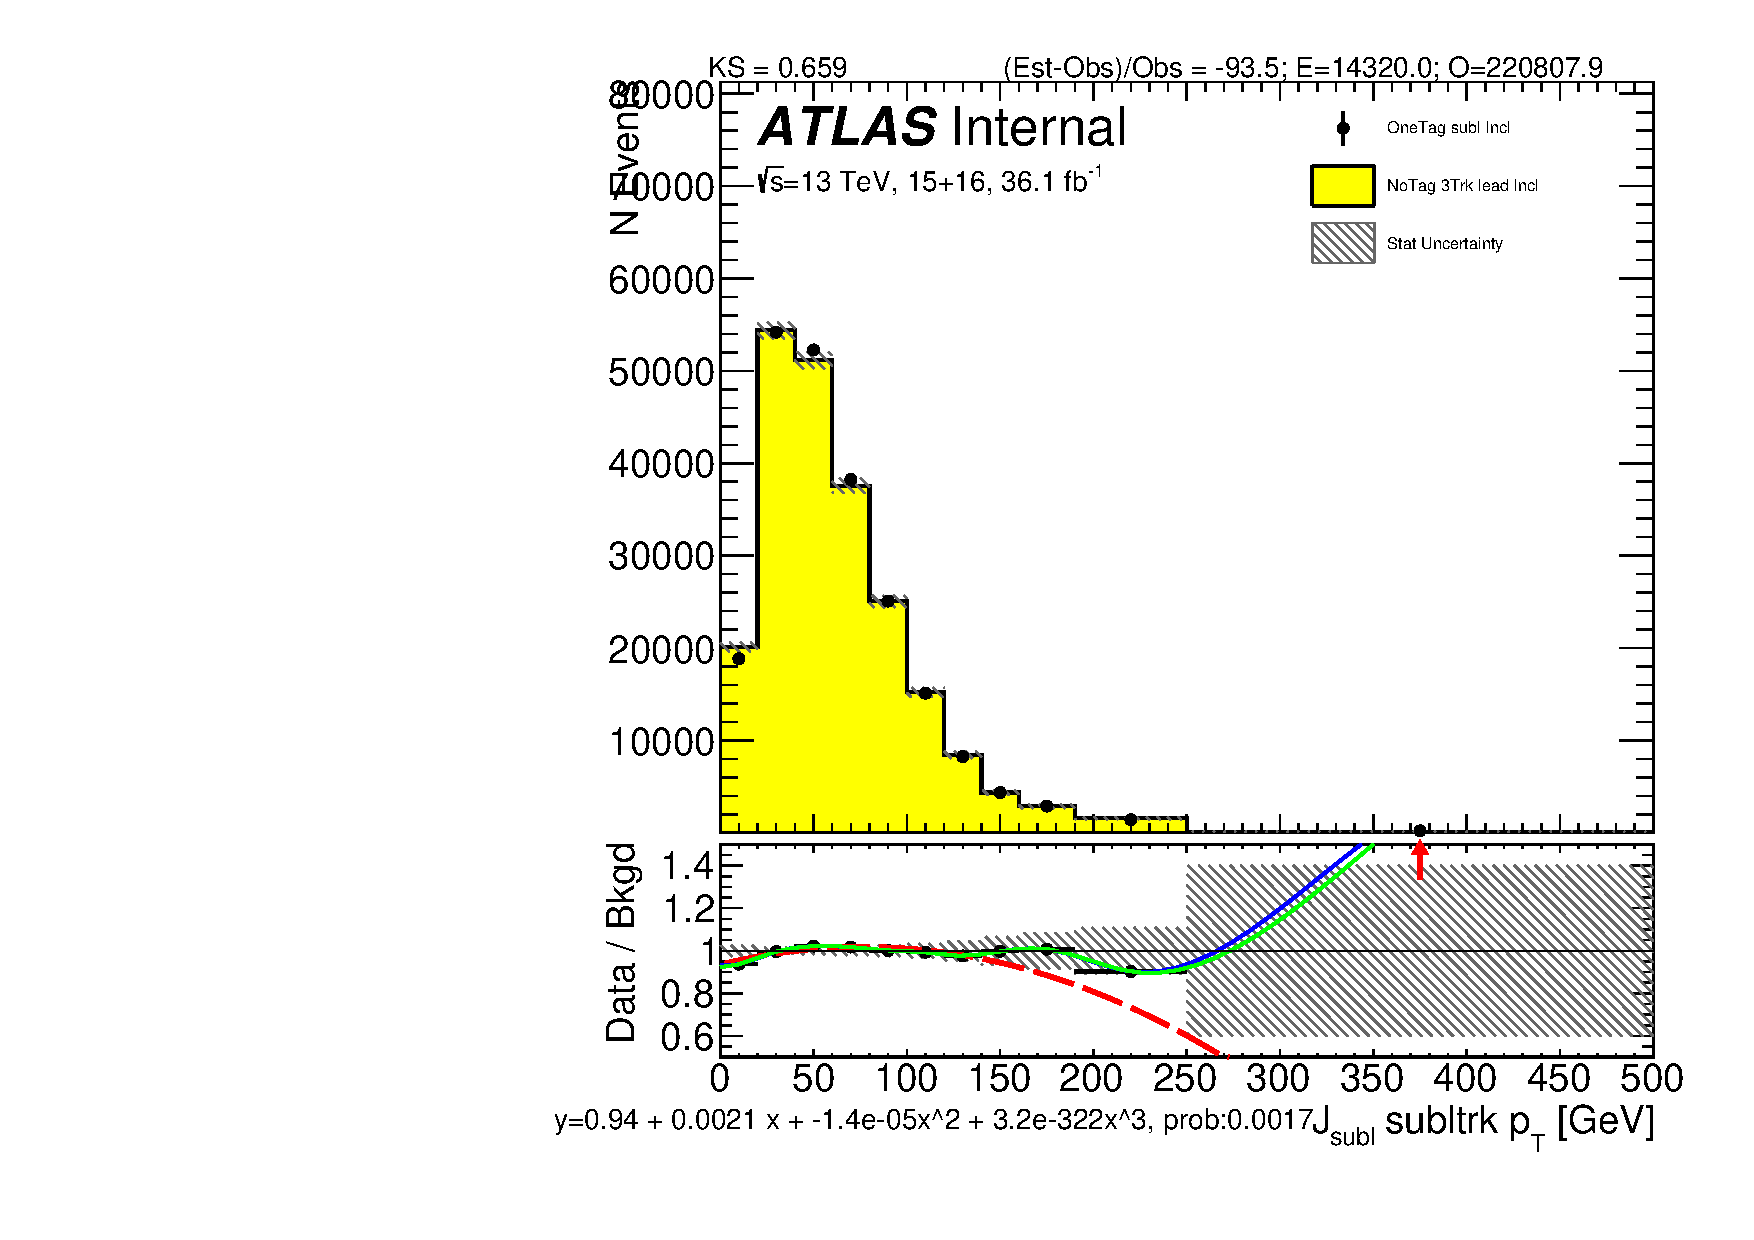
\includegraphics[width=0.25\textwidth,angle=-90]{figures/boosted/Reweight/Fits/Moriond_bkg_0_NoTag_3Trk_lead_Incl_sublHCand_trk1_Pt.pdf} \\
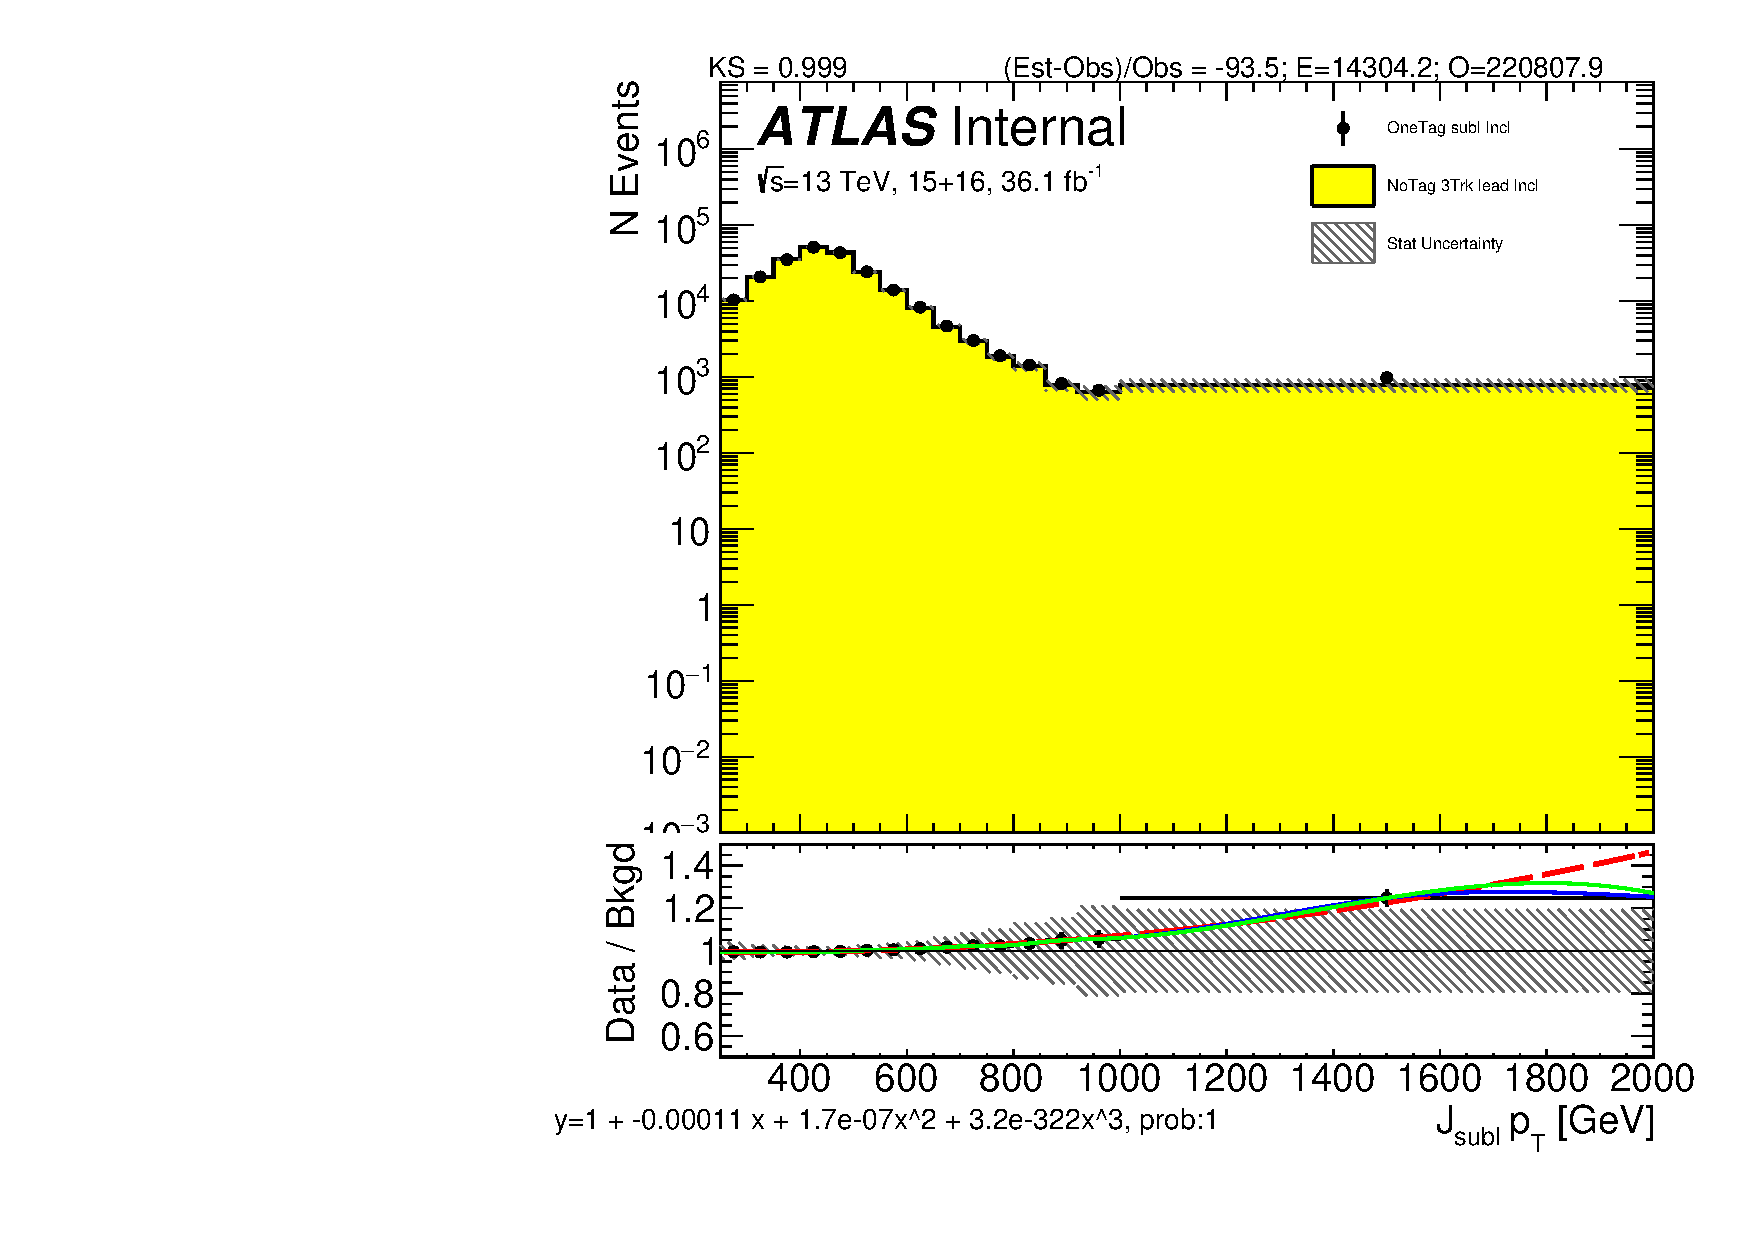
\includegraphics[width=0.25\textwidth,angle=-90]{figures/boosted/Reweight/Fits/Moriond_bkg_3_NoTag_3Trk_lead_Incl_sublHCand_Pt_m_1.pdf}
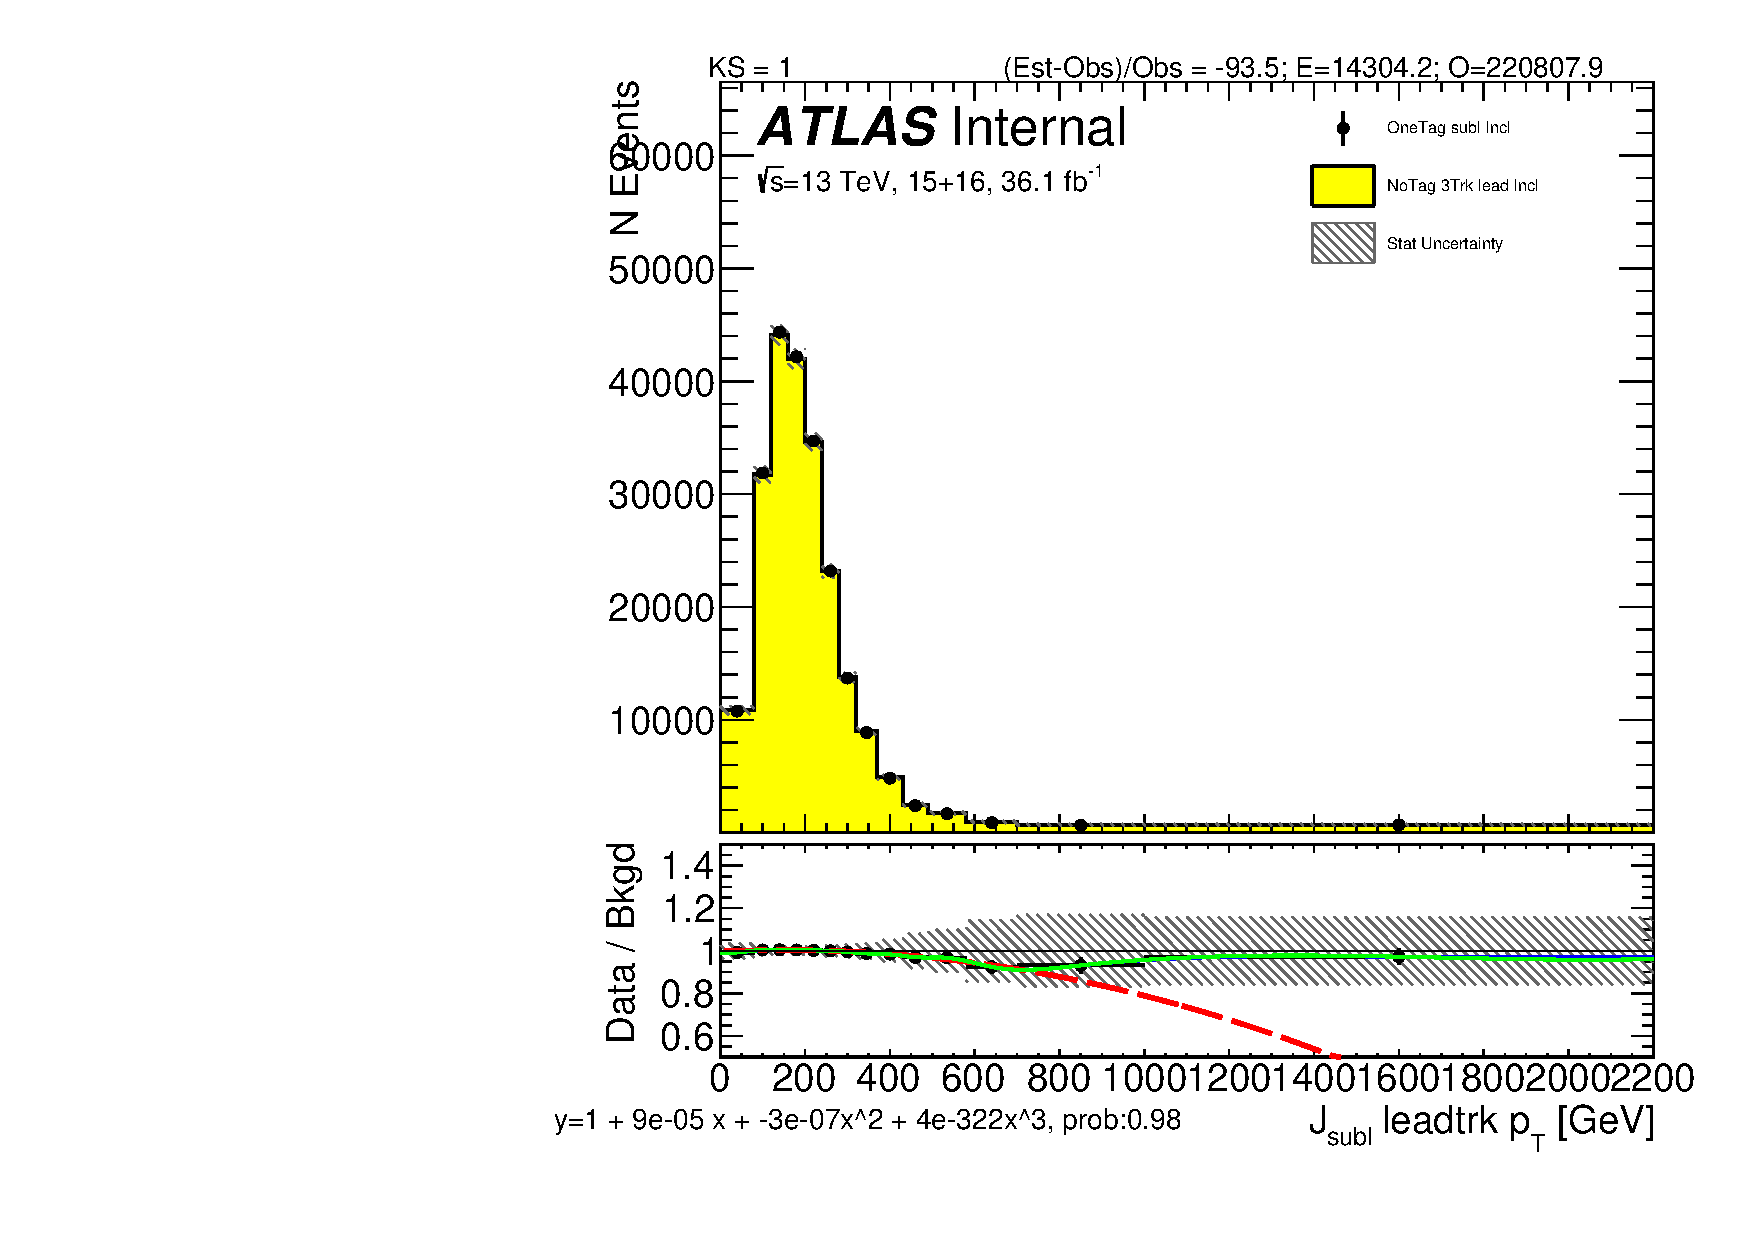
\includegraphics[width=0.25\textwidth,angle=-90]{figures/boosted/Reweight/Fits/Moriond_bkg_3_NoTag_3Trk_lead_Incl_sublHCand_trk0_Pt.pdf}
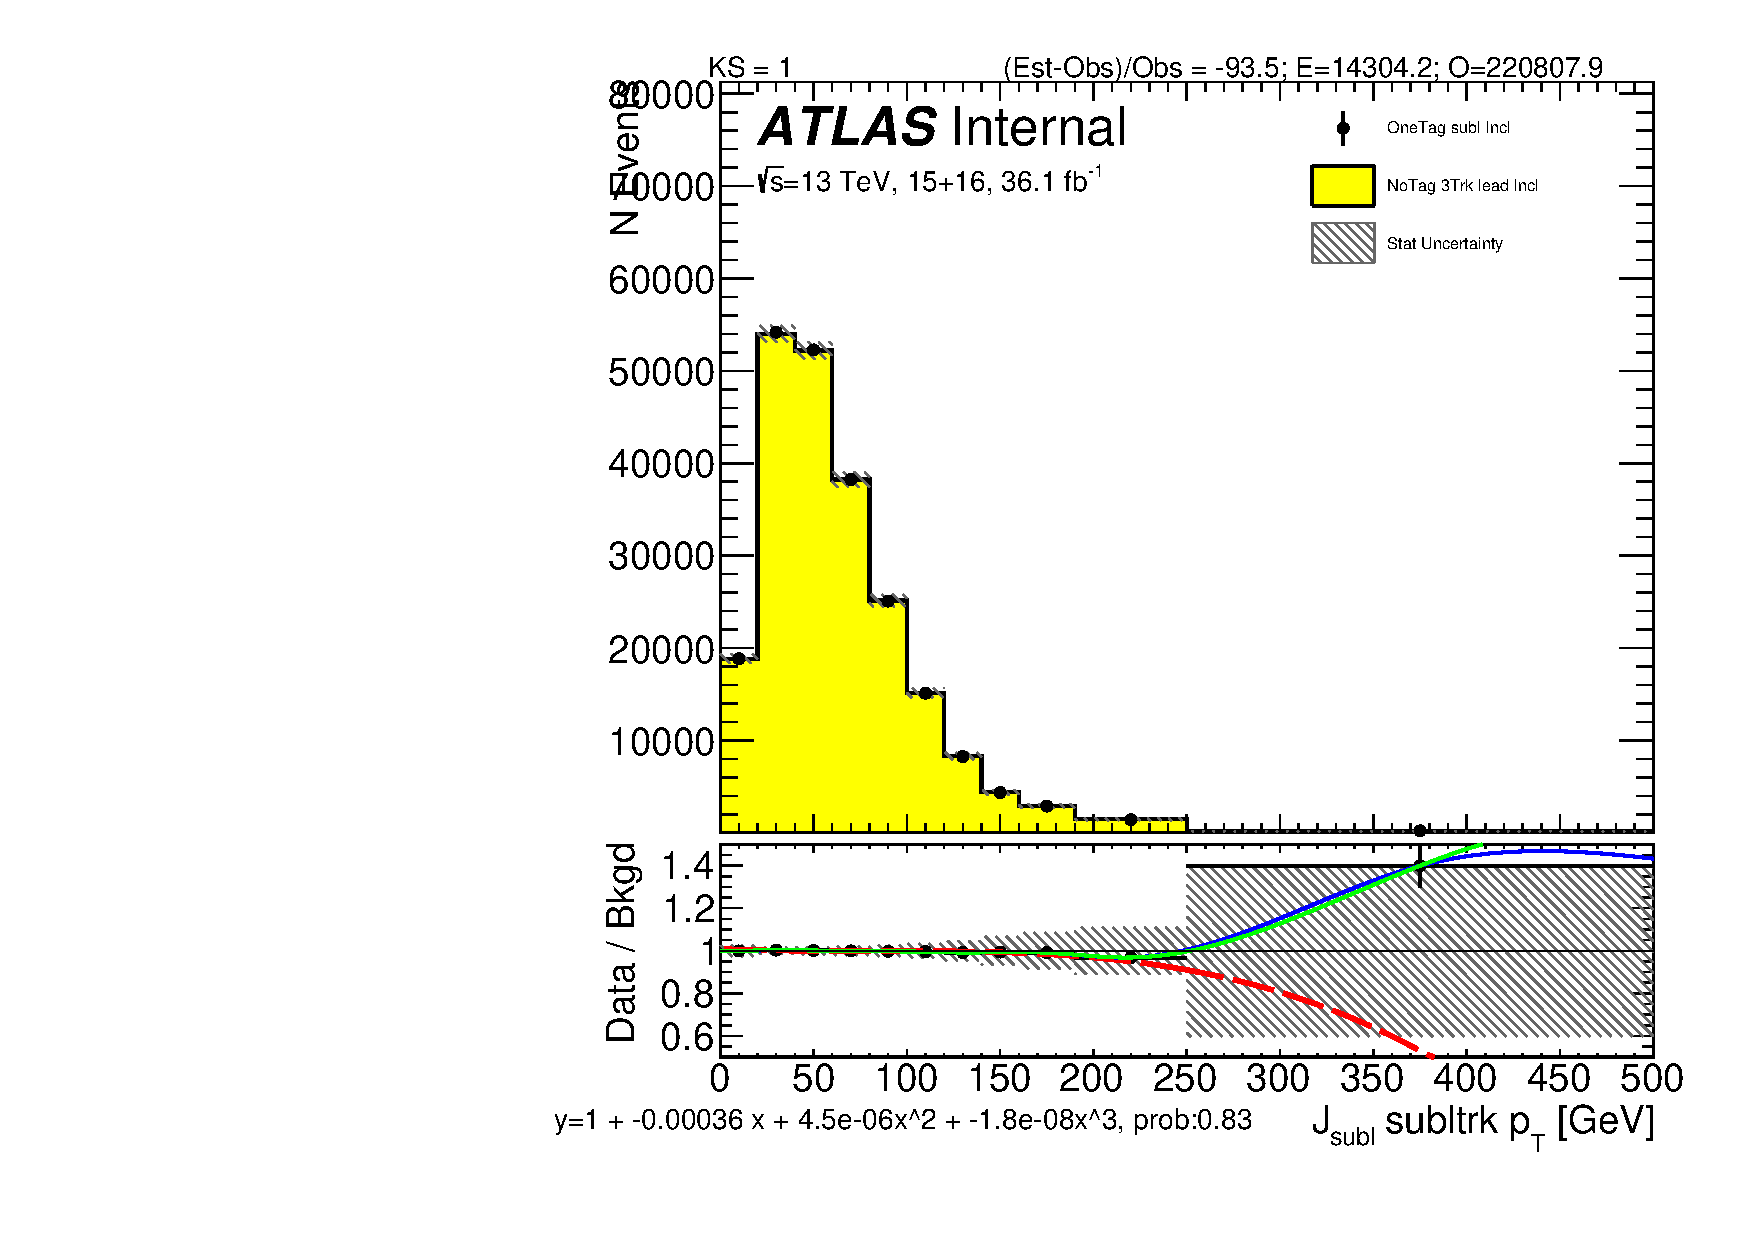
\includegraphics[width=0.25\textwidth,angle=-90]{figures/boosted/Reweight/Fits/Moriond_bkg_3_NoTag_3Trk_lead_Incl_sublHCand_trk1_Pt.pdf} \\
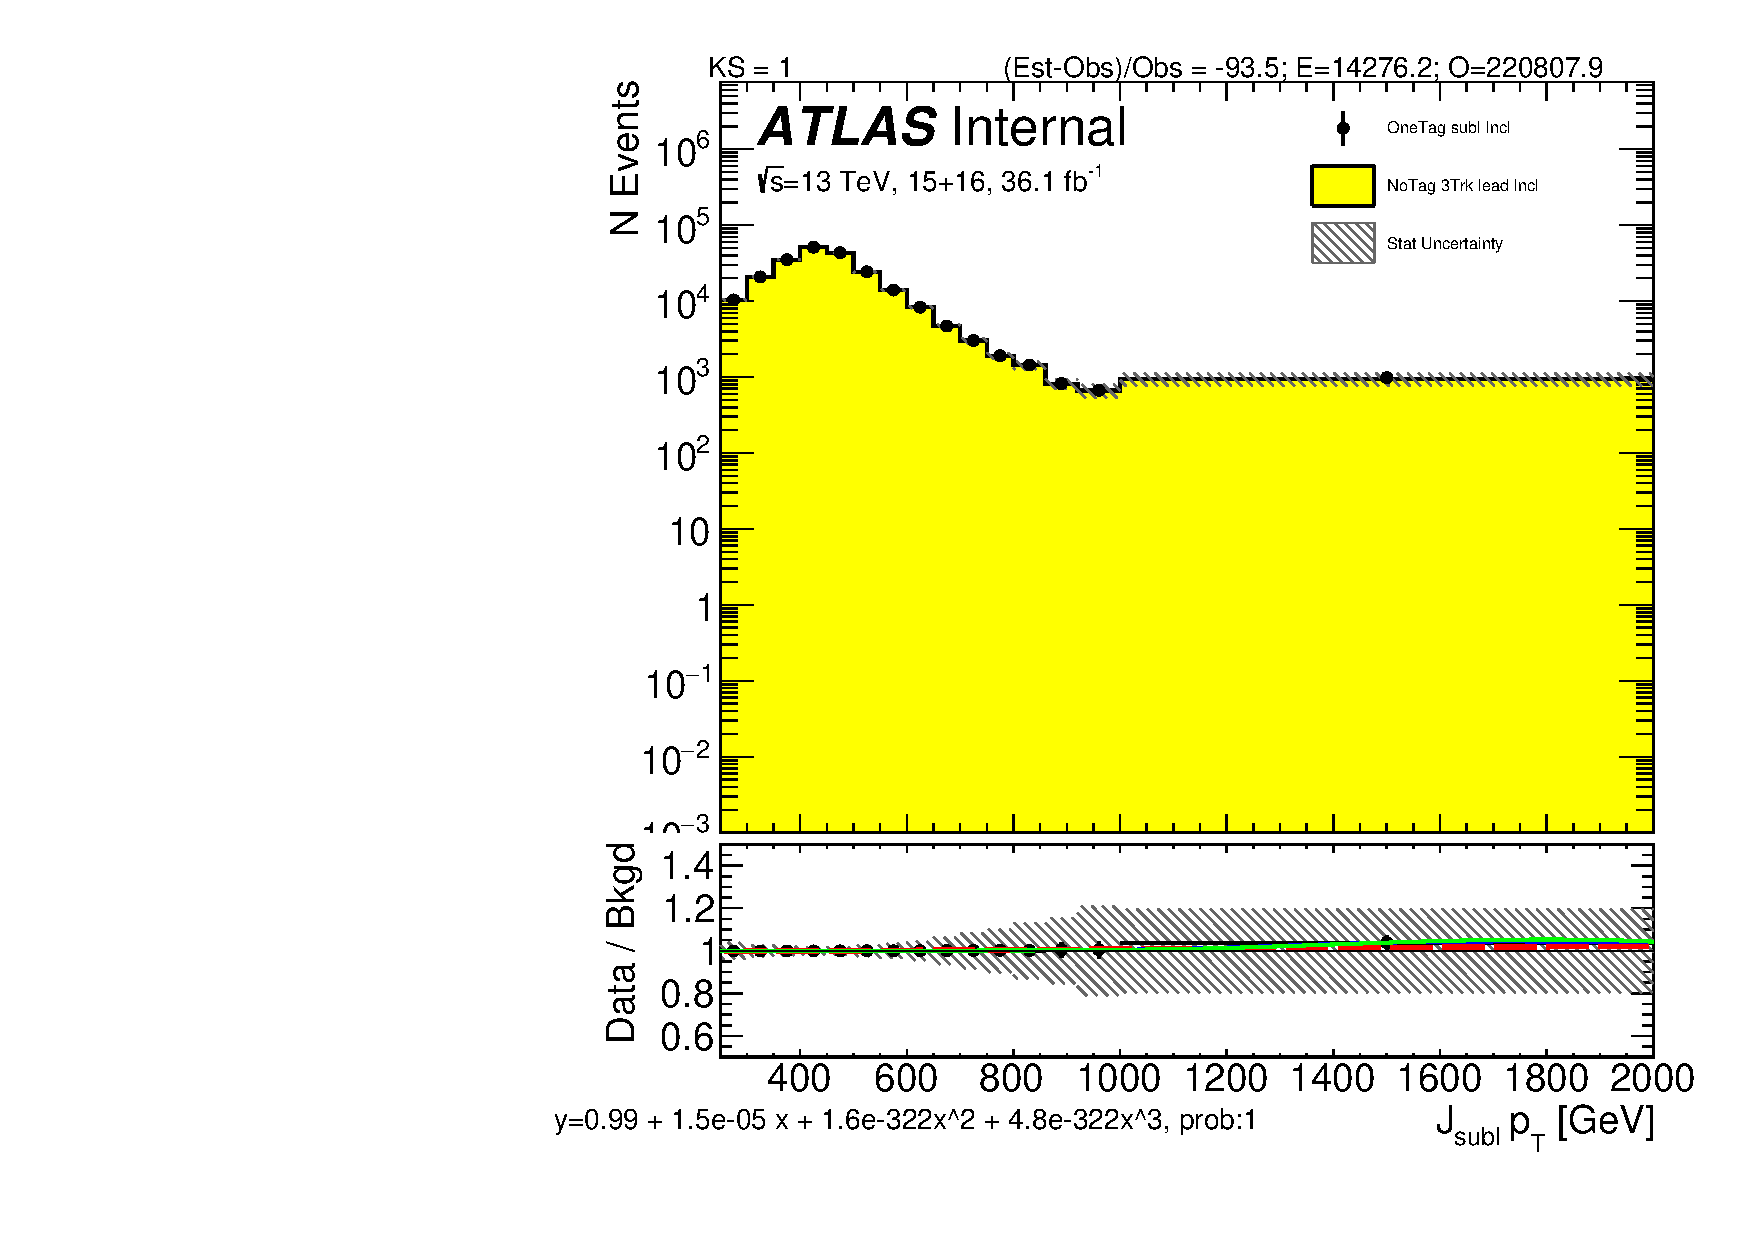
\includegraphics[width=0.25\textwidth,angle=-90]{figures/boosted/Reweight/Fits/Moriond_bkg_9_NoTag_3Trk_lead_Incl_sublHCand_Pt_m_1.pdf}
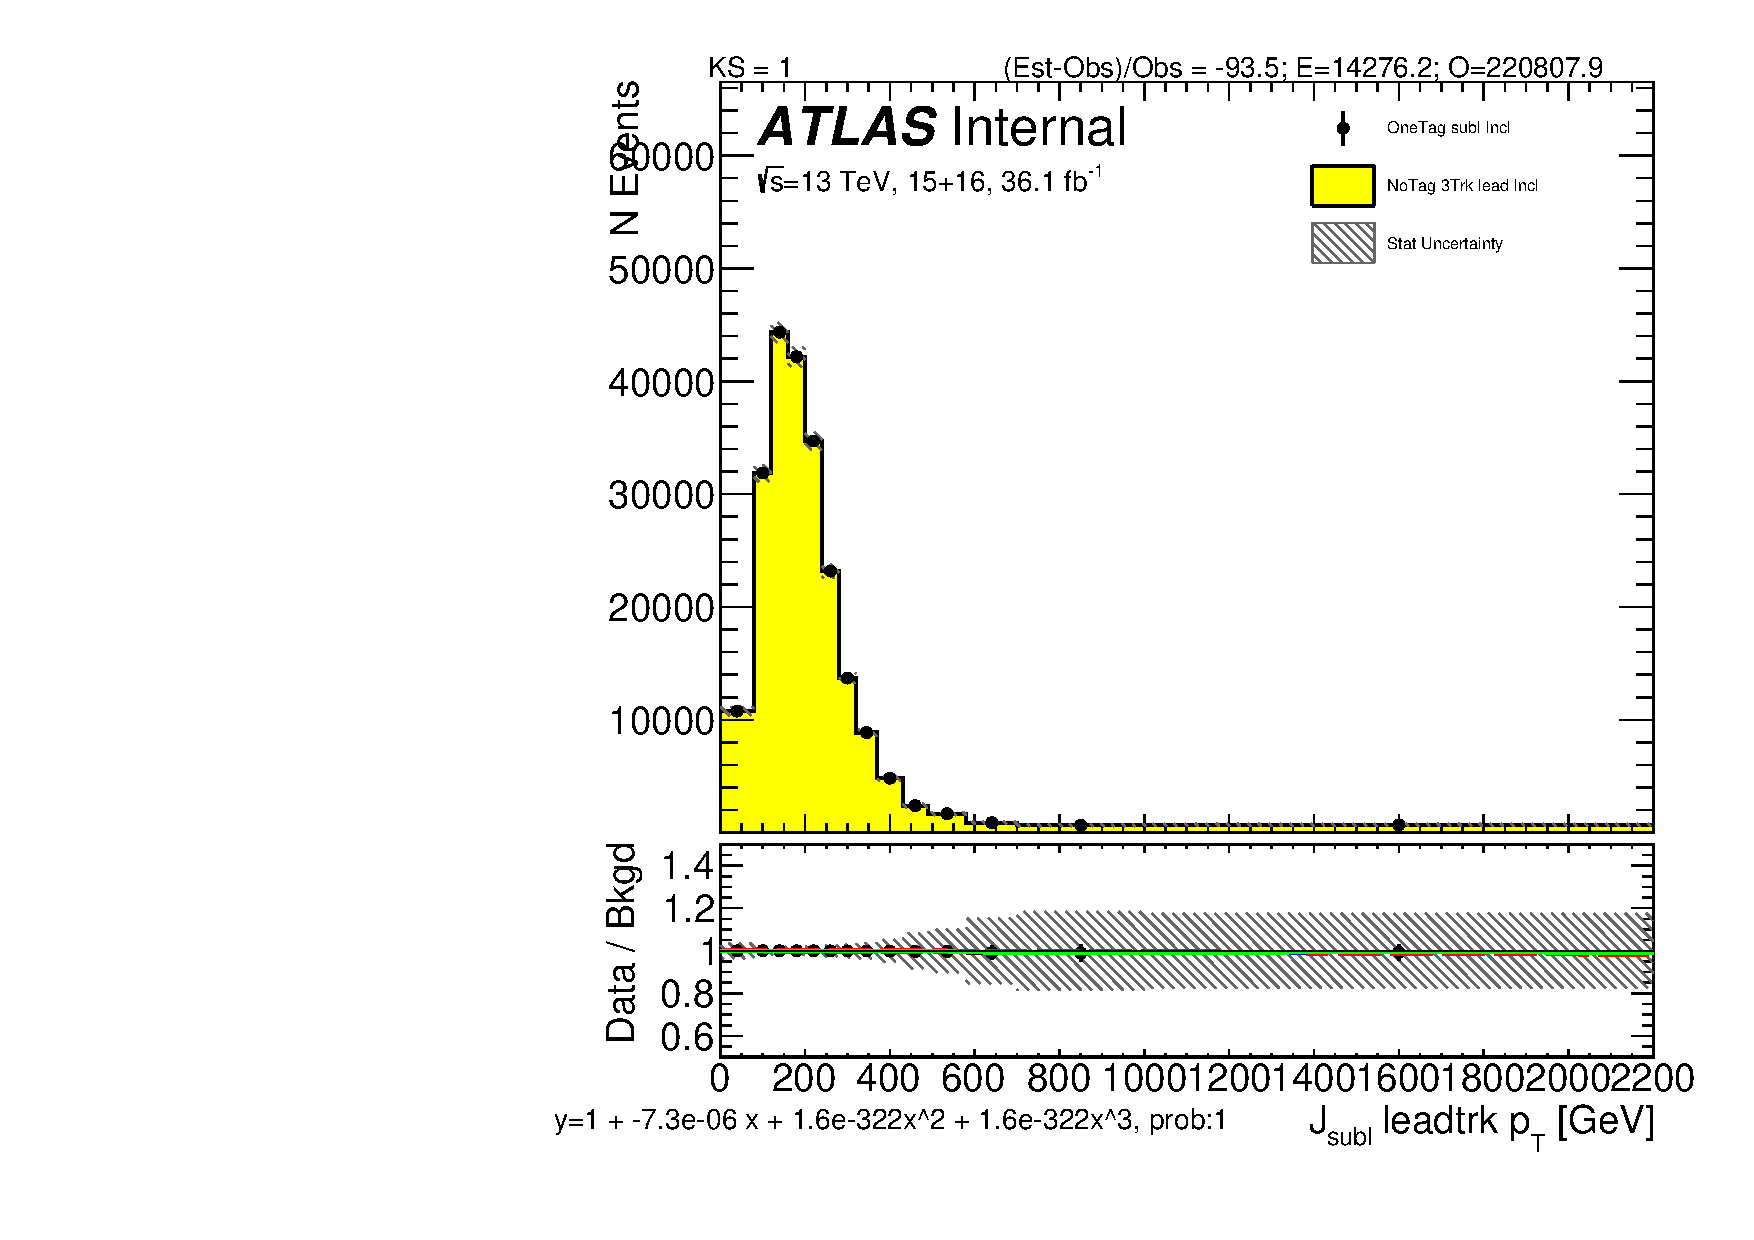
\includegraphics[width=0.25\textwidth,angle=-90]{figures/boosted/Reweight/Fits/Moriond_bkg_9_NoTag_3Trk_lead_Incl_sublHCand_trk0_Pt.pdf}
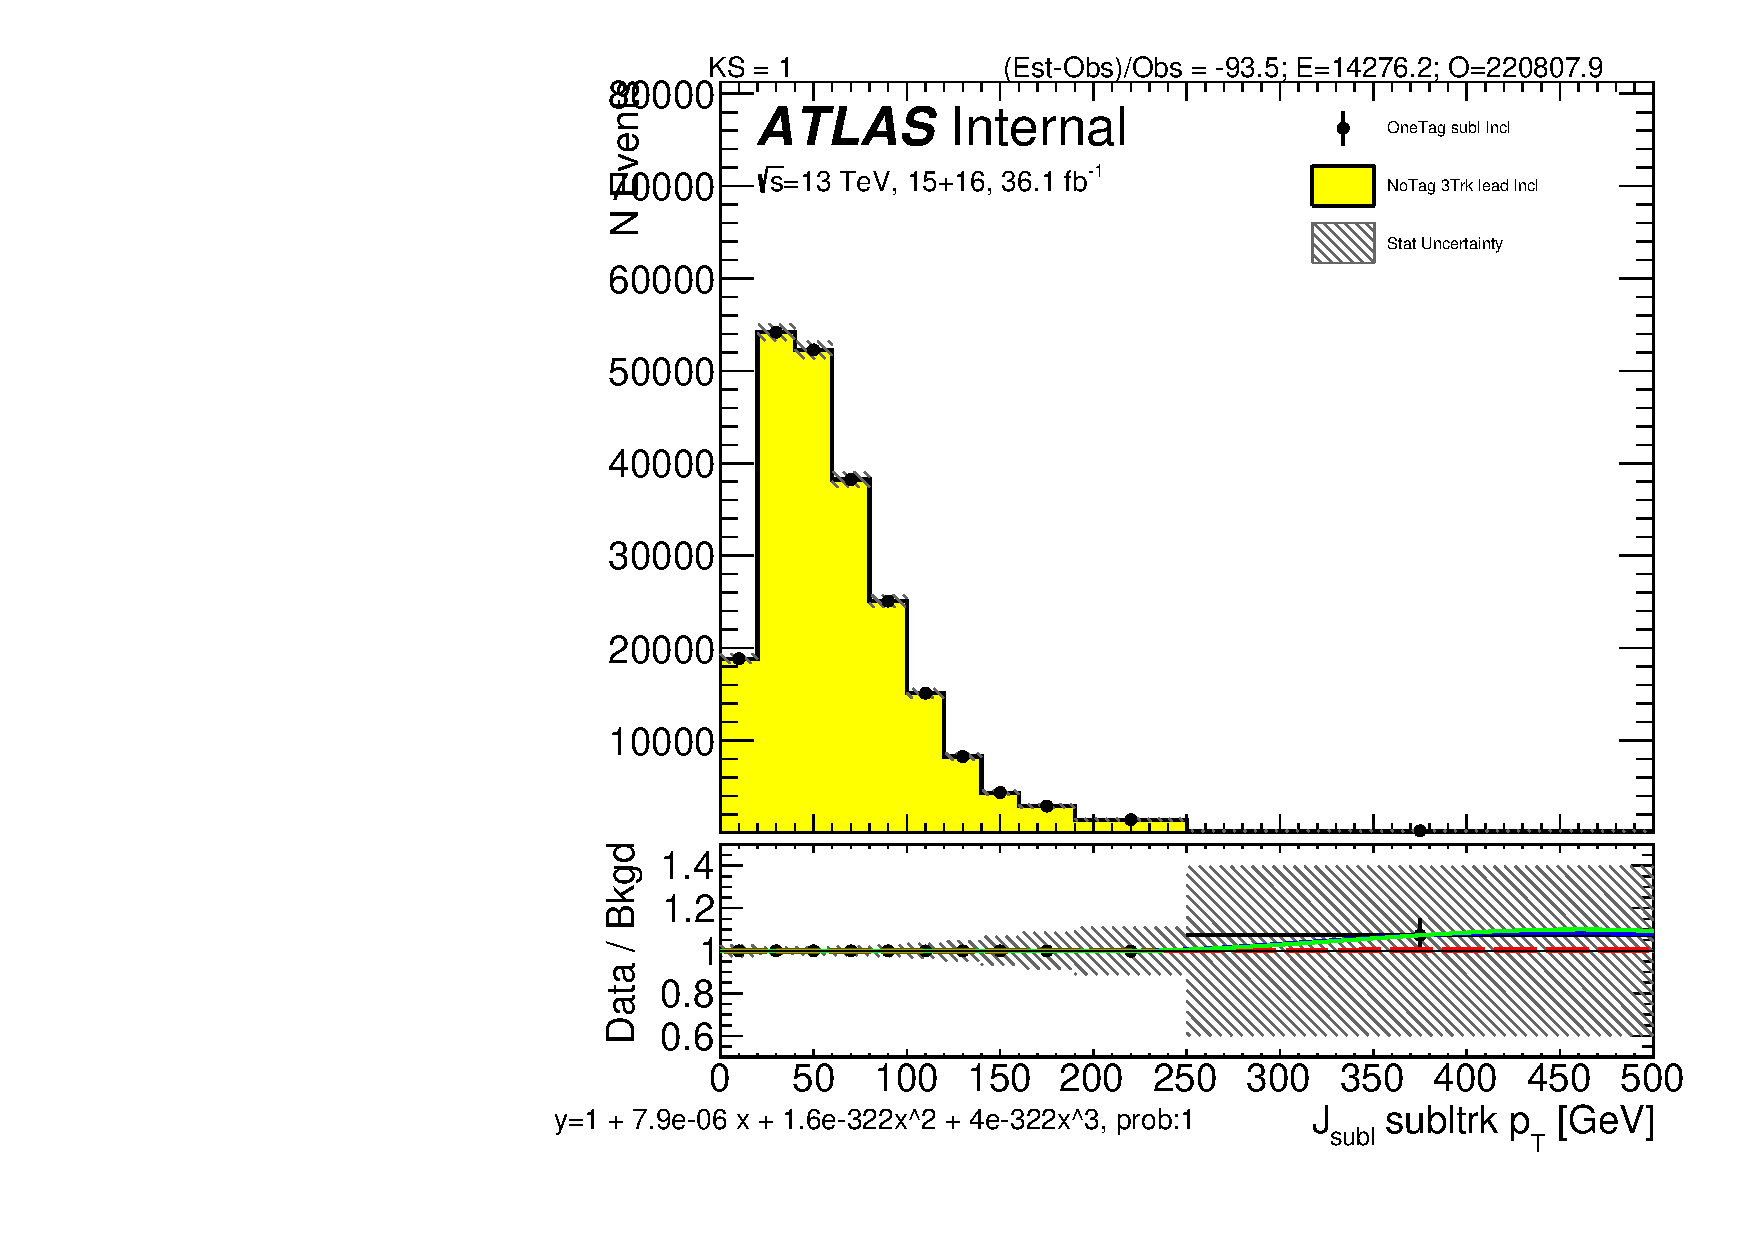
\includegraphics[width=0.25\textwidth,angle=-90]{figures/boosted/Reweight/Fits/Moriond_bkg_9_NoTag_3Trk_lead_Incl_sublHCand_trk1_Pt.pdf} \\
\caption{For $3b$ background estimate: the fits to the ratio of the data in the $2b$ category, of the subleading Higgs candidate $2b$-tagged events's subleading Higgs candidate distributions(black point), over the leading Higgs candidate $1b$-tagged events's subleading Higgs candidate distributions(yellow). Distributions and fits to the estimated QCD background for large-\R jet $p_{T}$ (left),  the large-\R jet's leading trackjet $p_T$ (middle), and large-\R jet's subleading trackjet $p_T$ (right) are shown.  Figures are before reweighting (top row), after the first iteration(second row), after the fourth iteration(third row), and after the last iteration (bottom row). The green line is the spline fit; the red line is a polynomial fit; the blue line is the spline interpolation.}
\label{fig:rw-3b-lead}
\end{center}
\end{figure*}

\begin{figure*}[htbp!]
\begin{center}
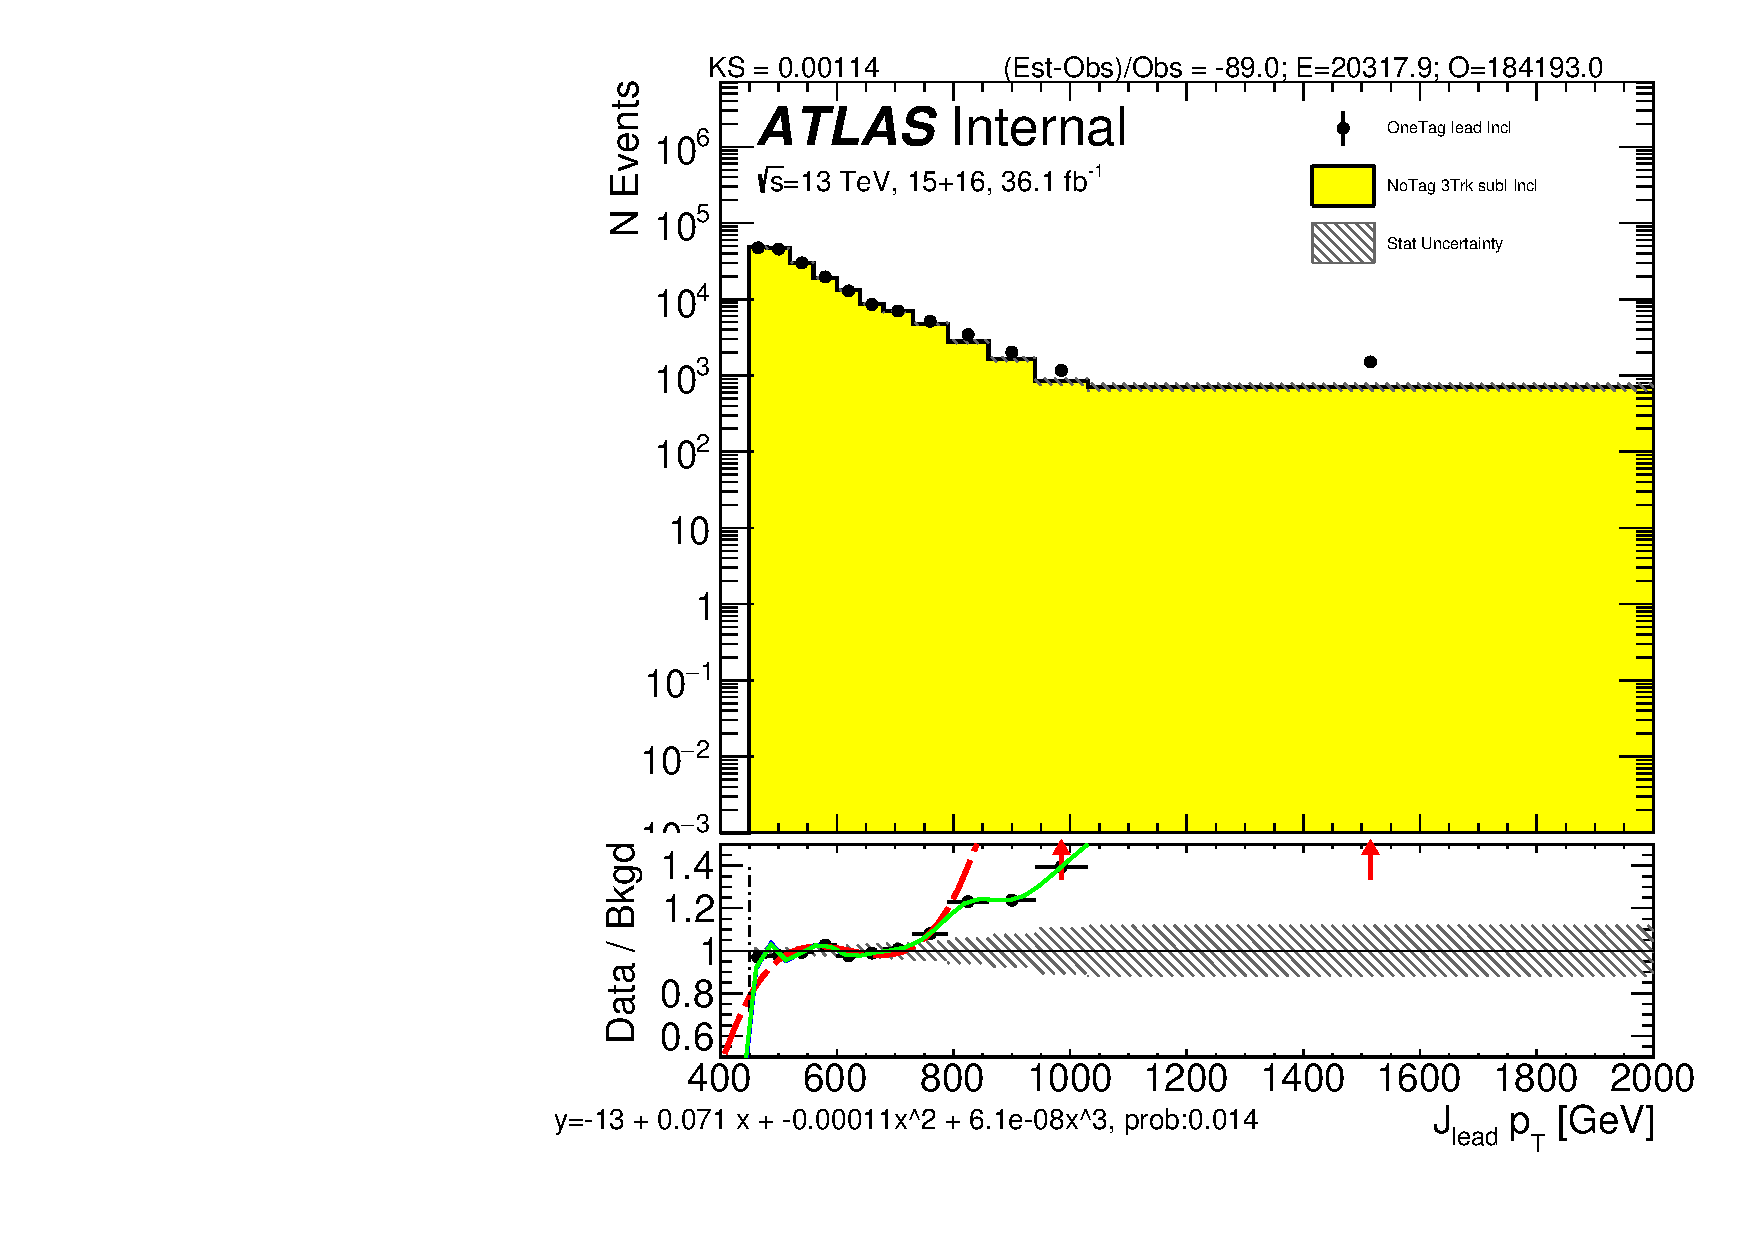
\includegraphics[width=0.25\textwidth,angle=-90]{figures/boosted/Reweight/Fits/Moriond_NoTag_3Trk_subl_Incl_leadHCand_Pt_m_1.pdf}
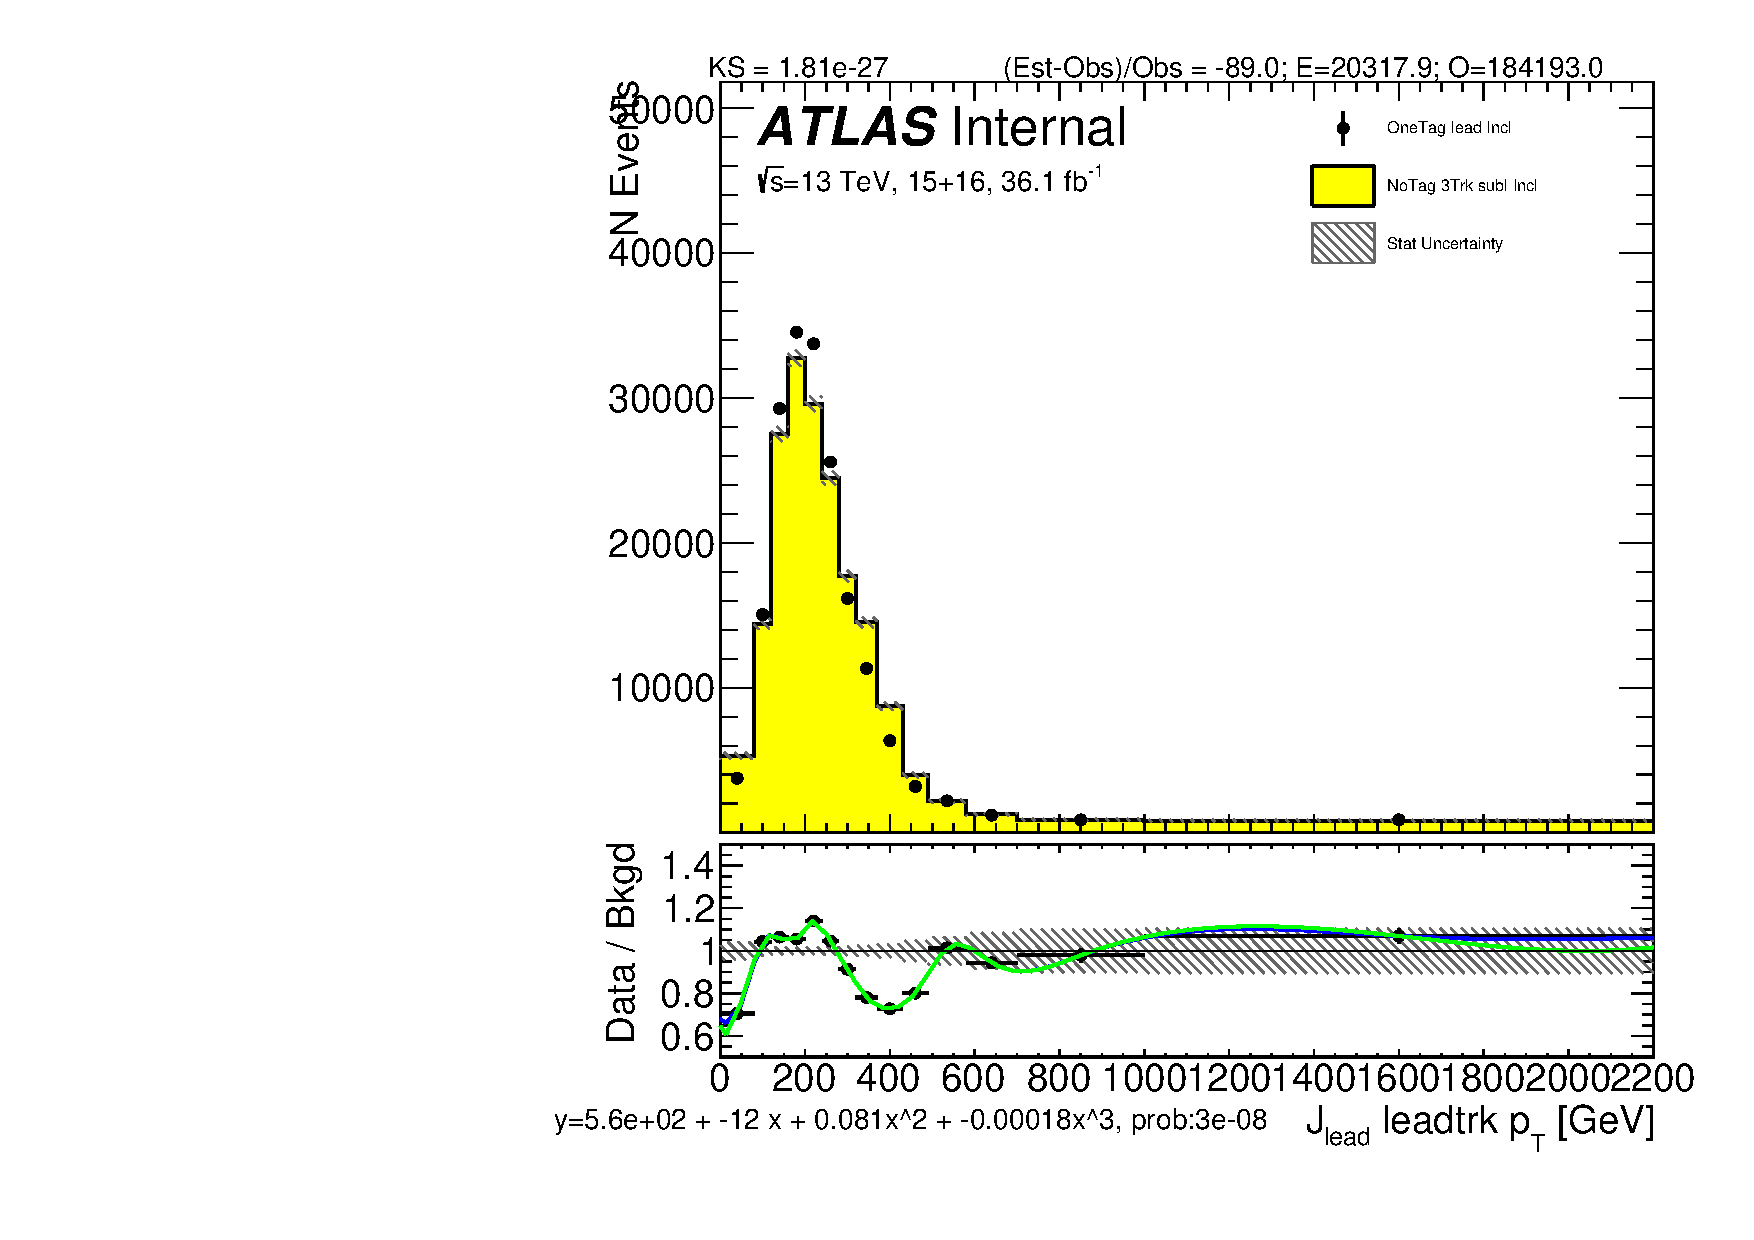
\includegraphics[width=0.25\textwidth,angle=-90]{figures/boosted/Reweight/Fits/Moriond_NoTag_3Trk_subl_Incl_leadHCand_trk0_Pt.pdf}
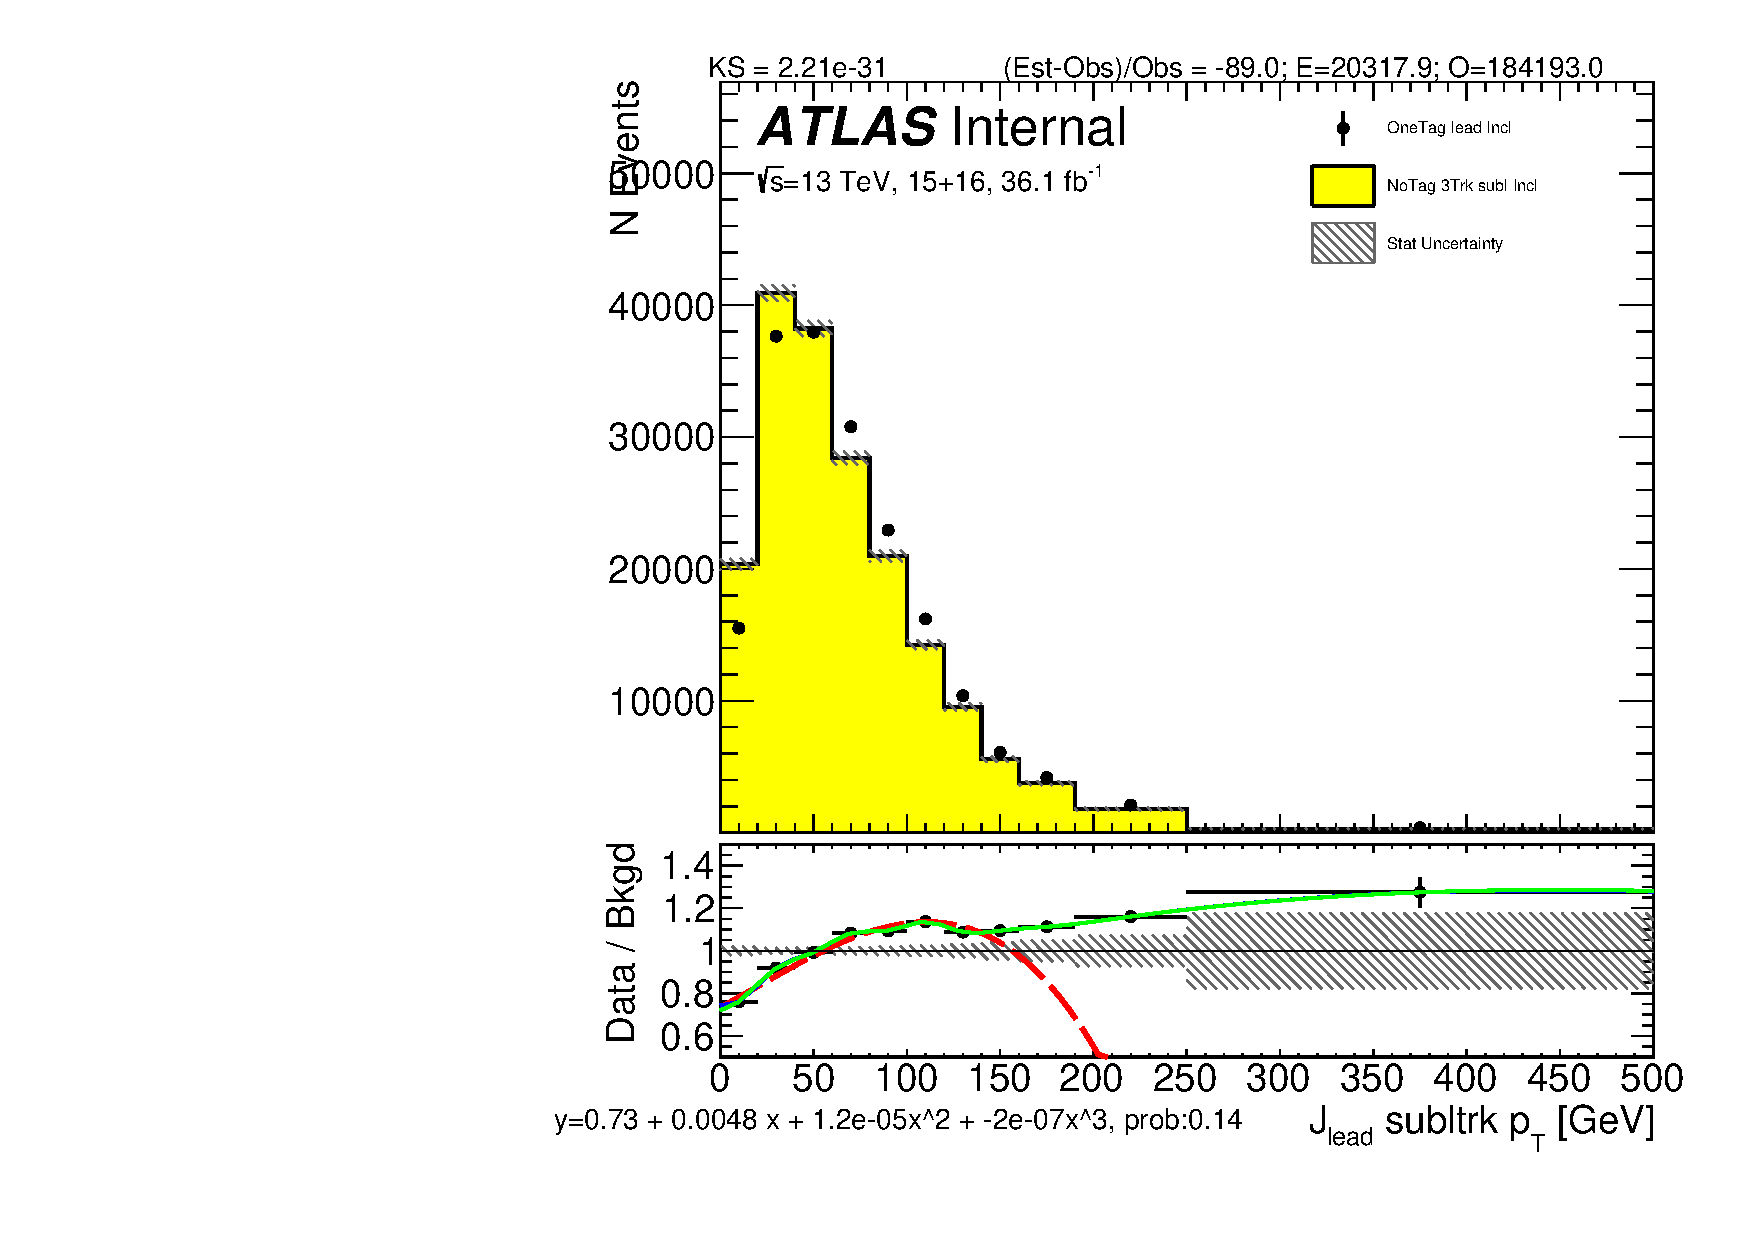
\includegraphics[width=0.25\textwidth,angle=-90]{figures/boosted/Reweight/Fits/Moriond_NoTag_3Trk_subl_Incl_leadHCand_trk1_Pt.pdf} \\
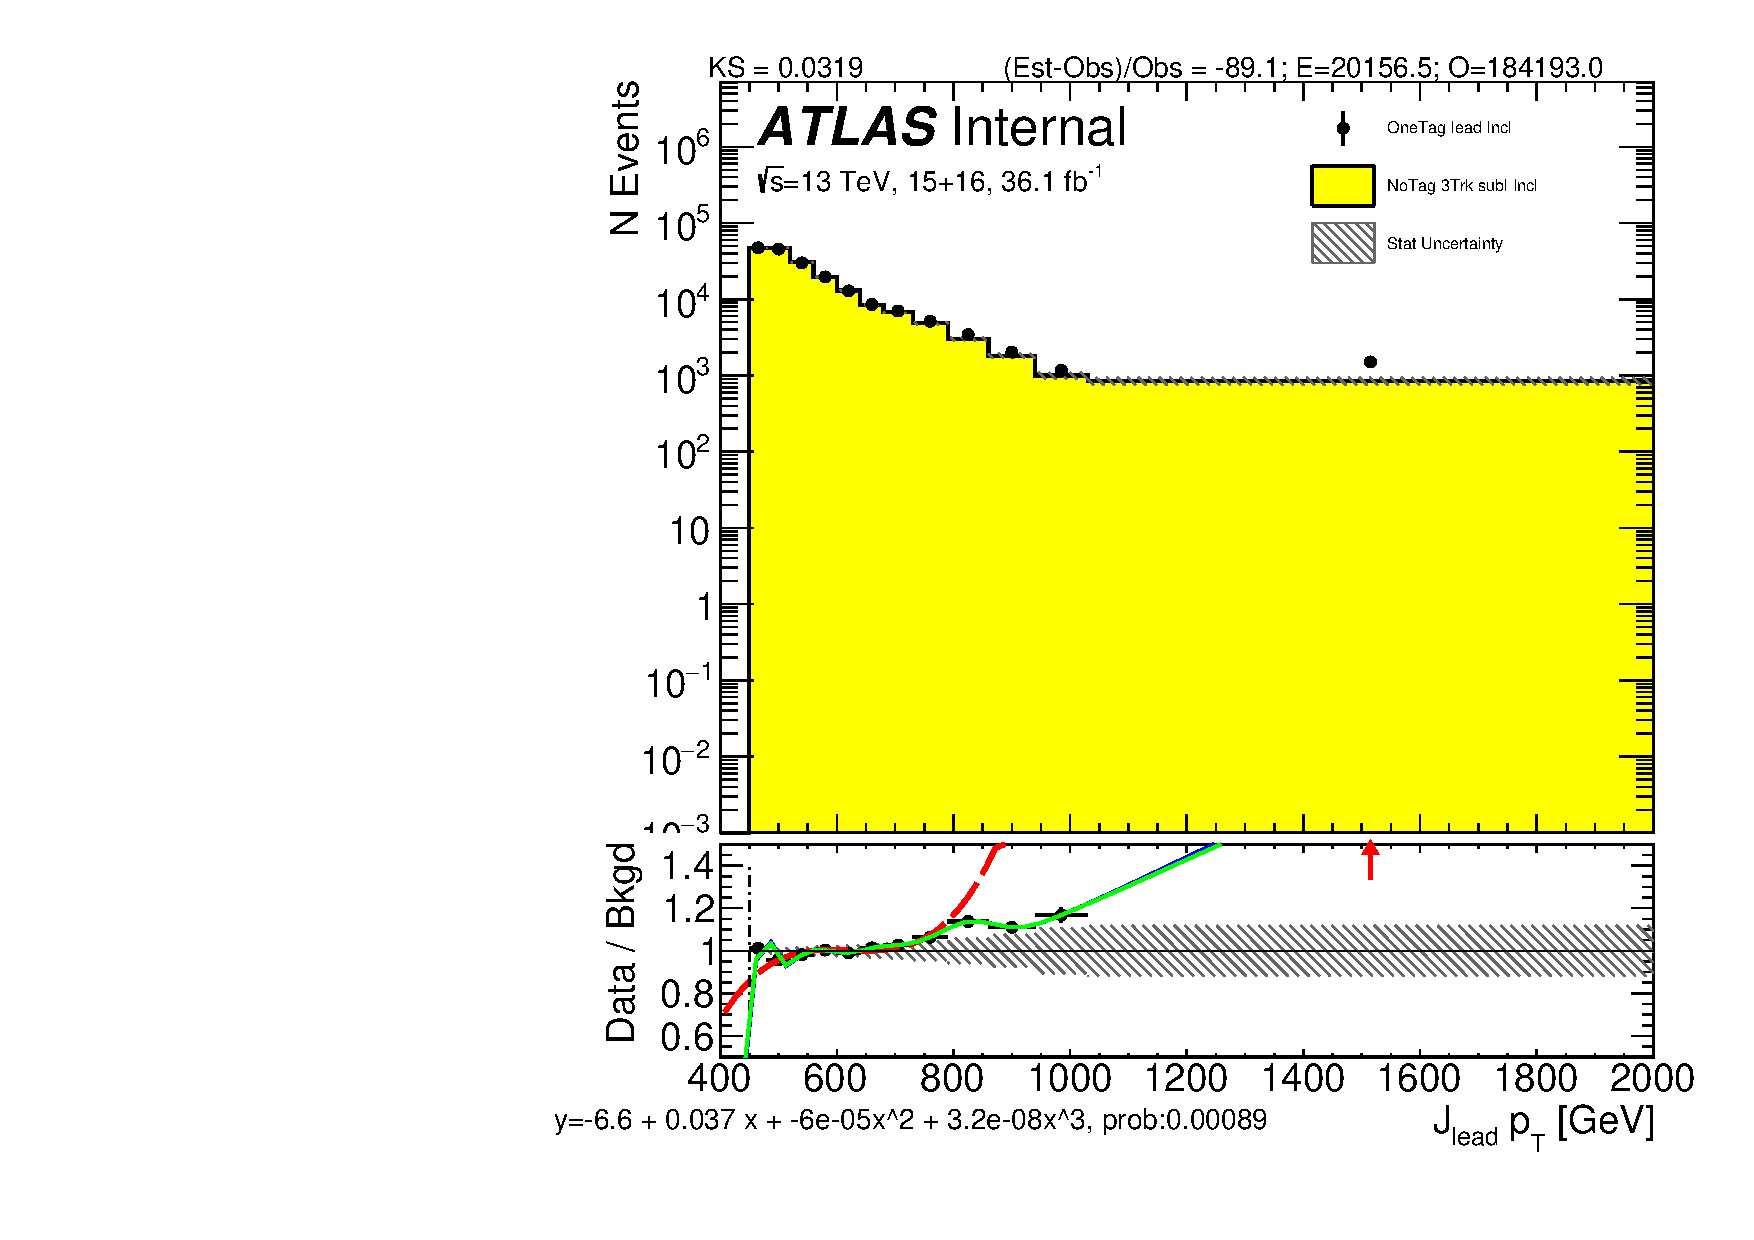
\includegraphics[width=0.25\textwidth,angle=-90]{figures/boosted/Reweight/Fits/Moriond_bkg_0_NoTag_3Trk_subl_Incl_leadHCand_Pt_m_1.pdf}
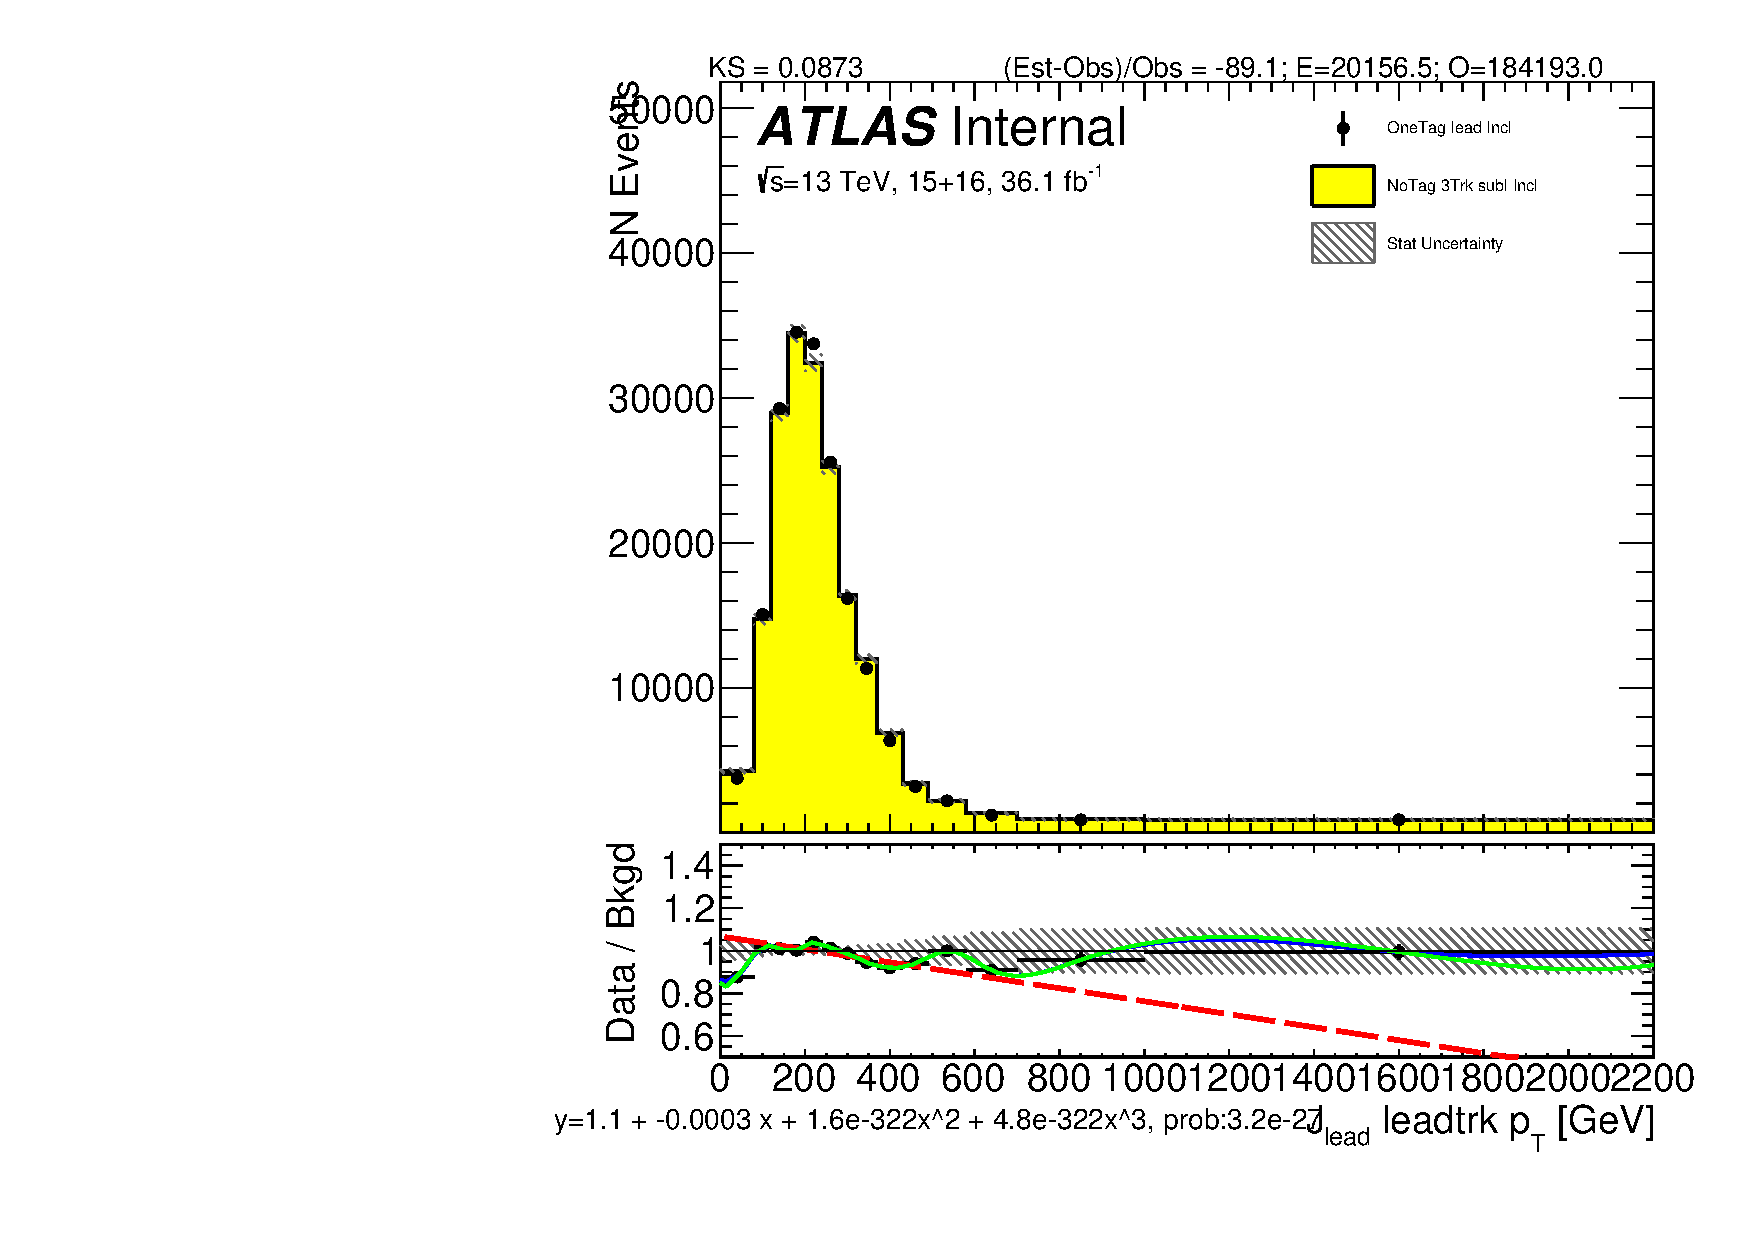
\includegraphics[width=0.25\textwidth,angle=-90]{figures/boosted/Reweight/Fits/Moriond_bkg_0_NoTag_3Trk_subl_Incl_leadHCand_trk0_Pt.pdf}
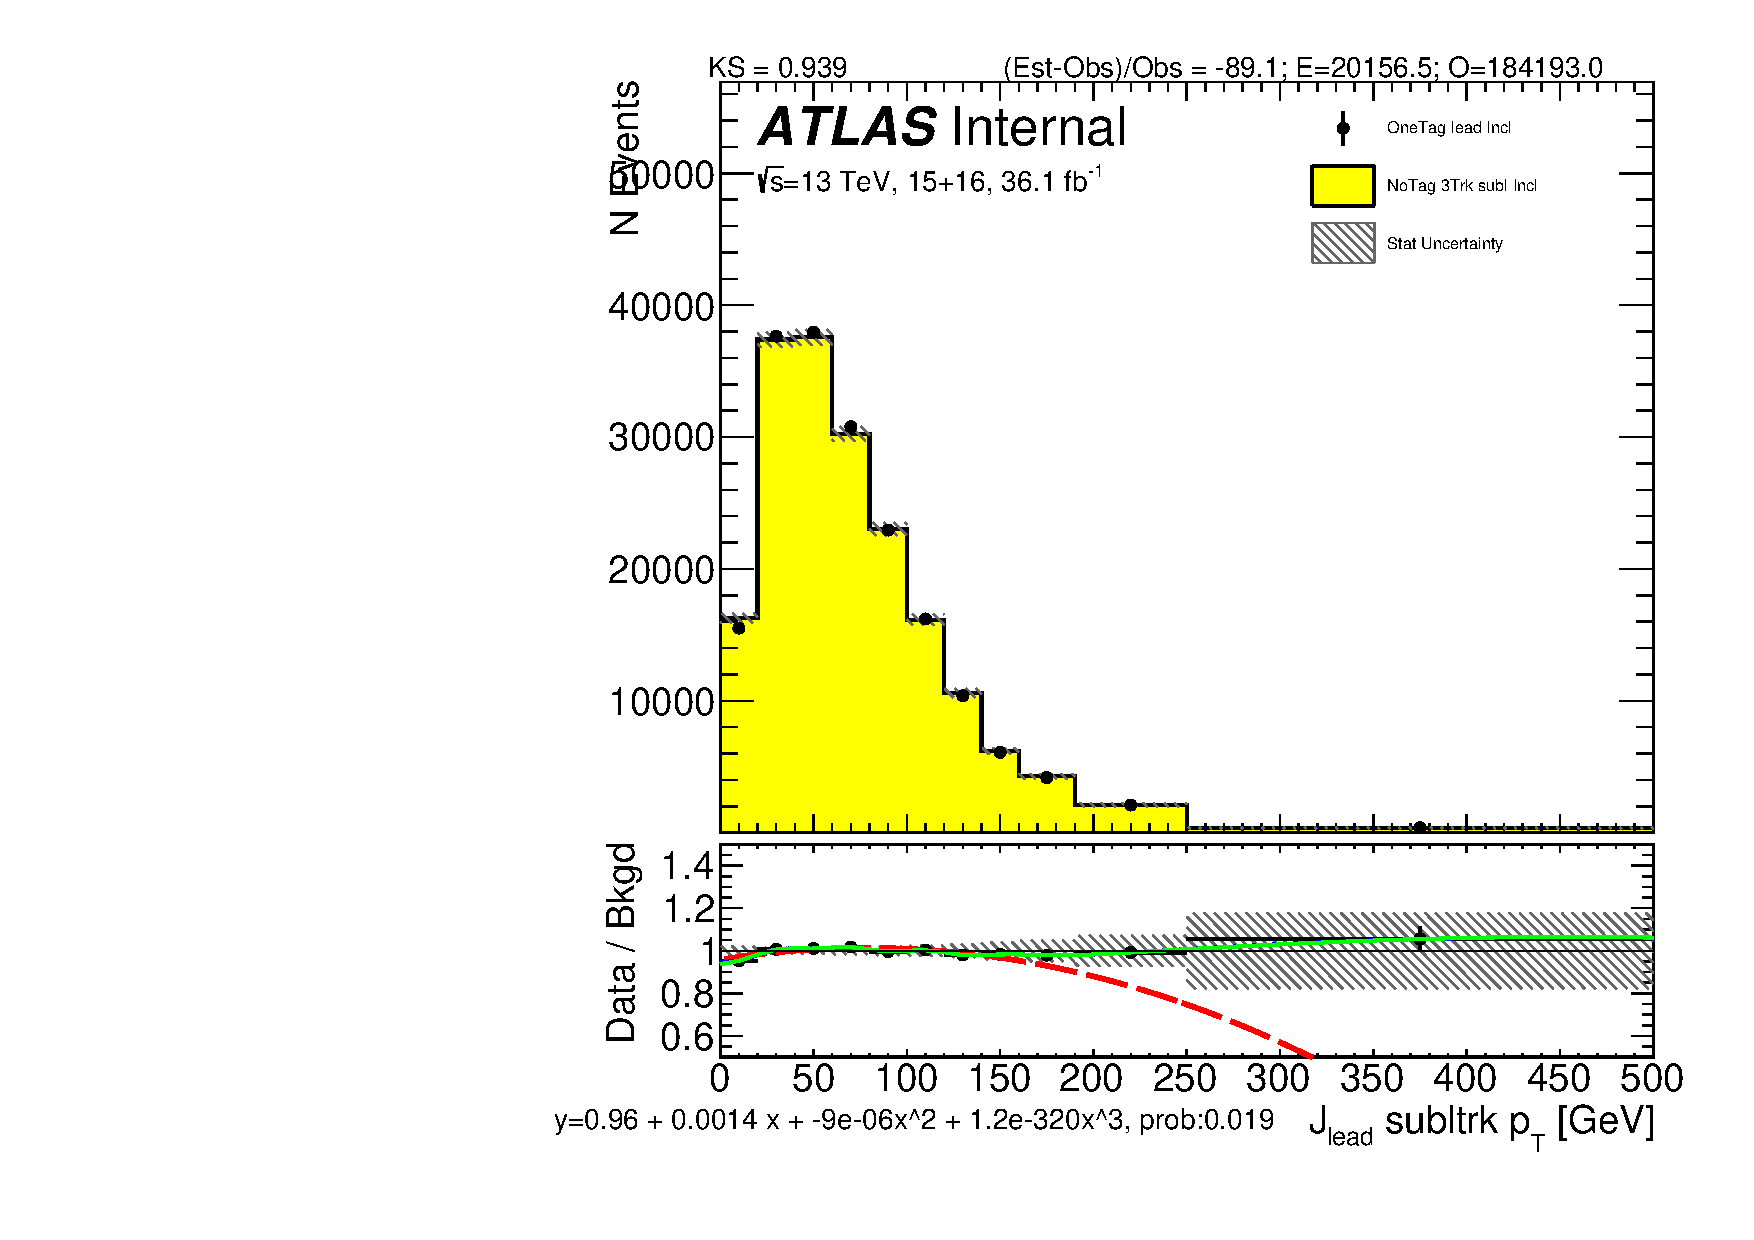
\includegraphics[width=0.25\textwidth,angle=-90]{figures/boosted/Reweight/Fits/Moriond_bkg_0_NoTag_3Trk_subl_Incl_leadHCand_trk1_Pt.pdf} \\
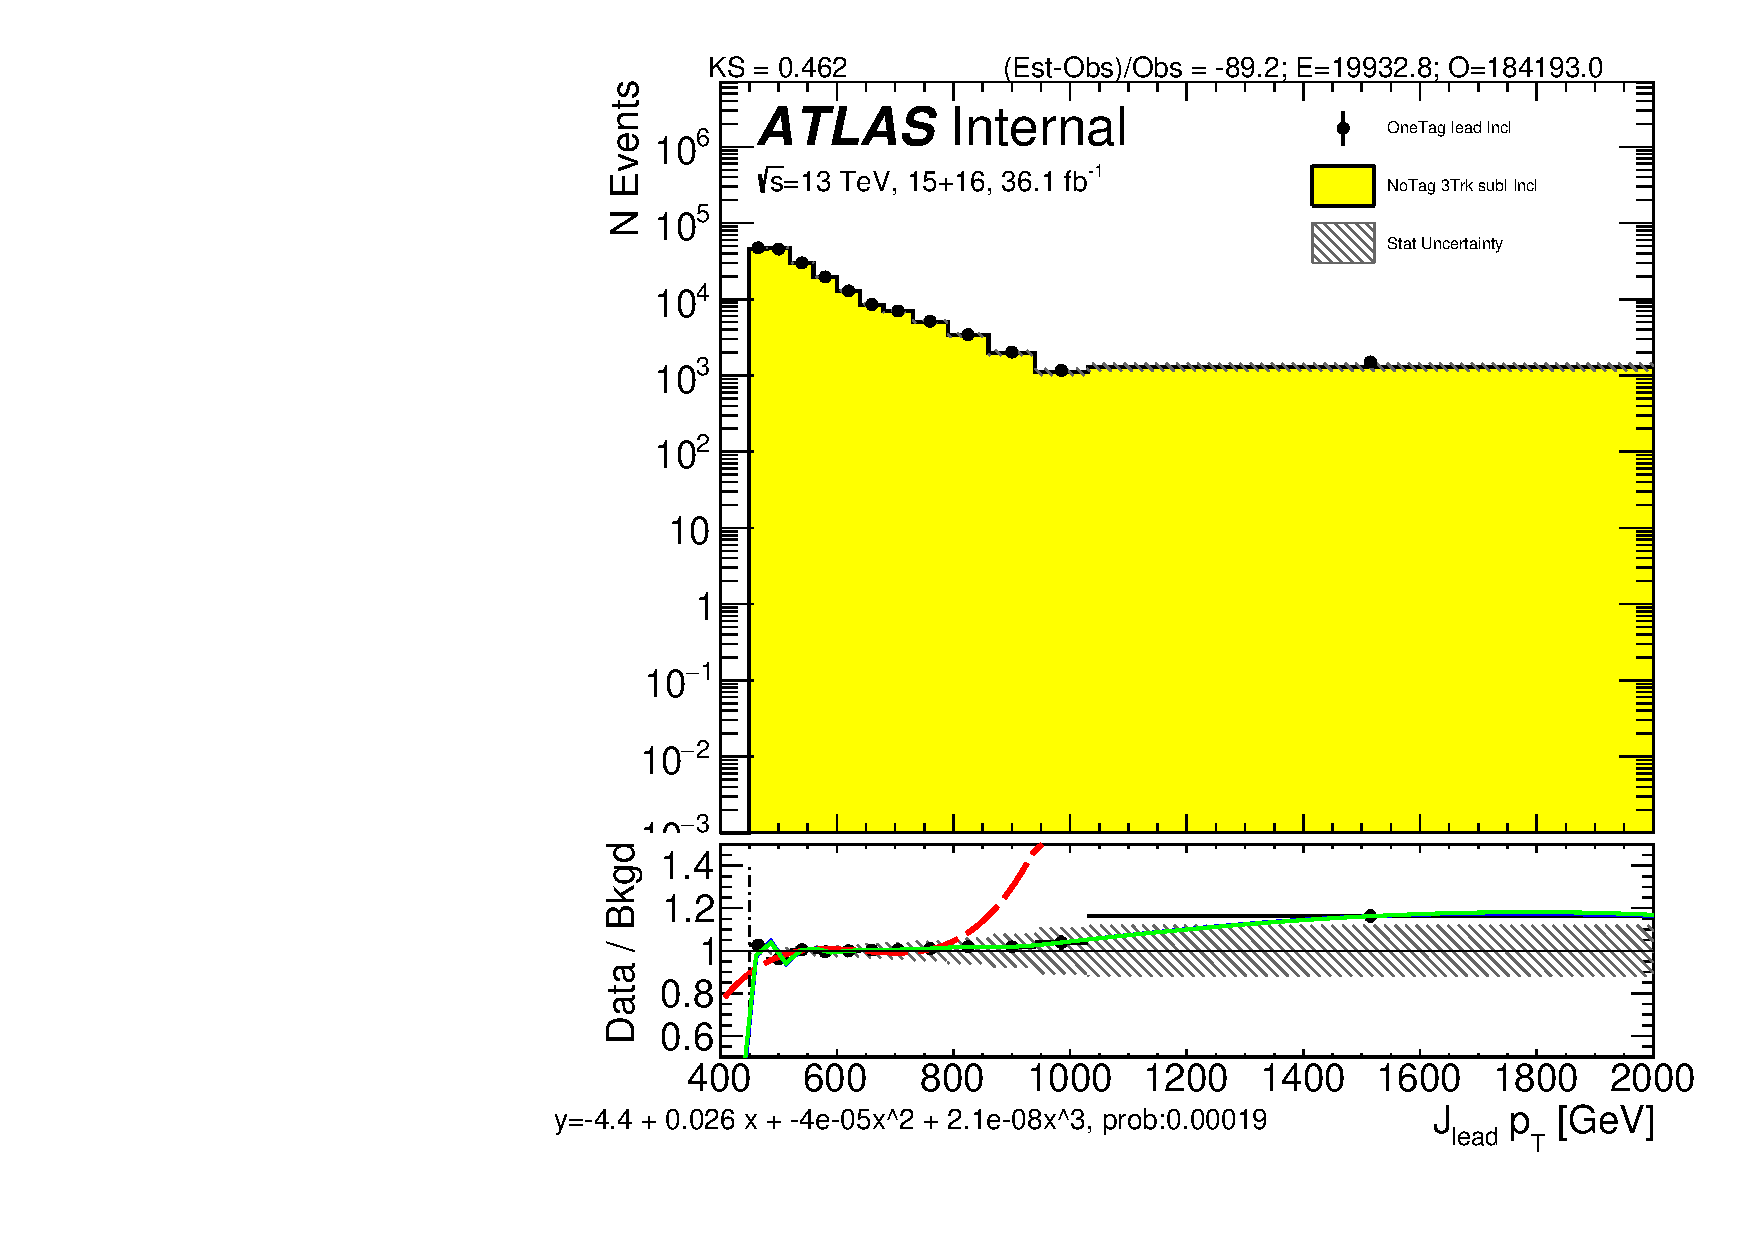
\includegraphics[width=0.25\textwidth,angle=-90]{figures/boosted/Reweight/Fits/Moriond_bkg_3_NoTag_3Trk_subl_Incl_leadHCand_Pt_m_1.pdf}
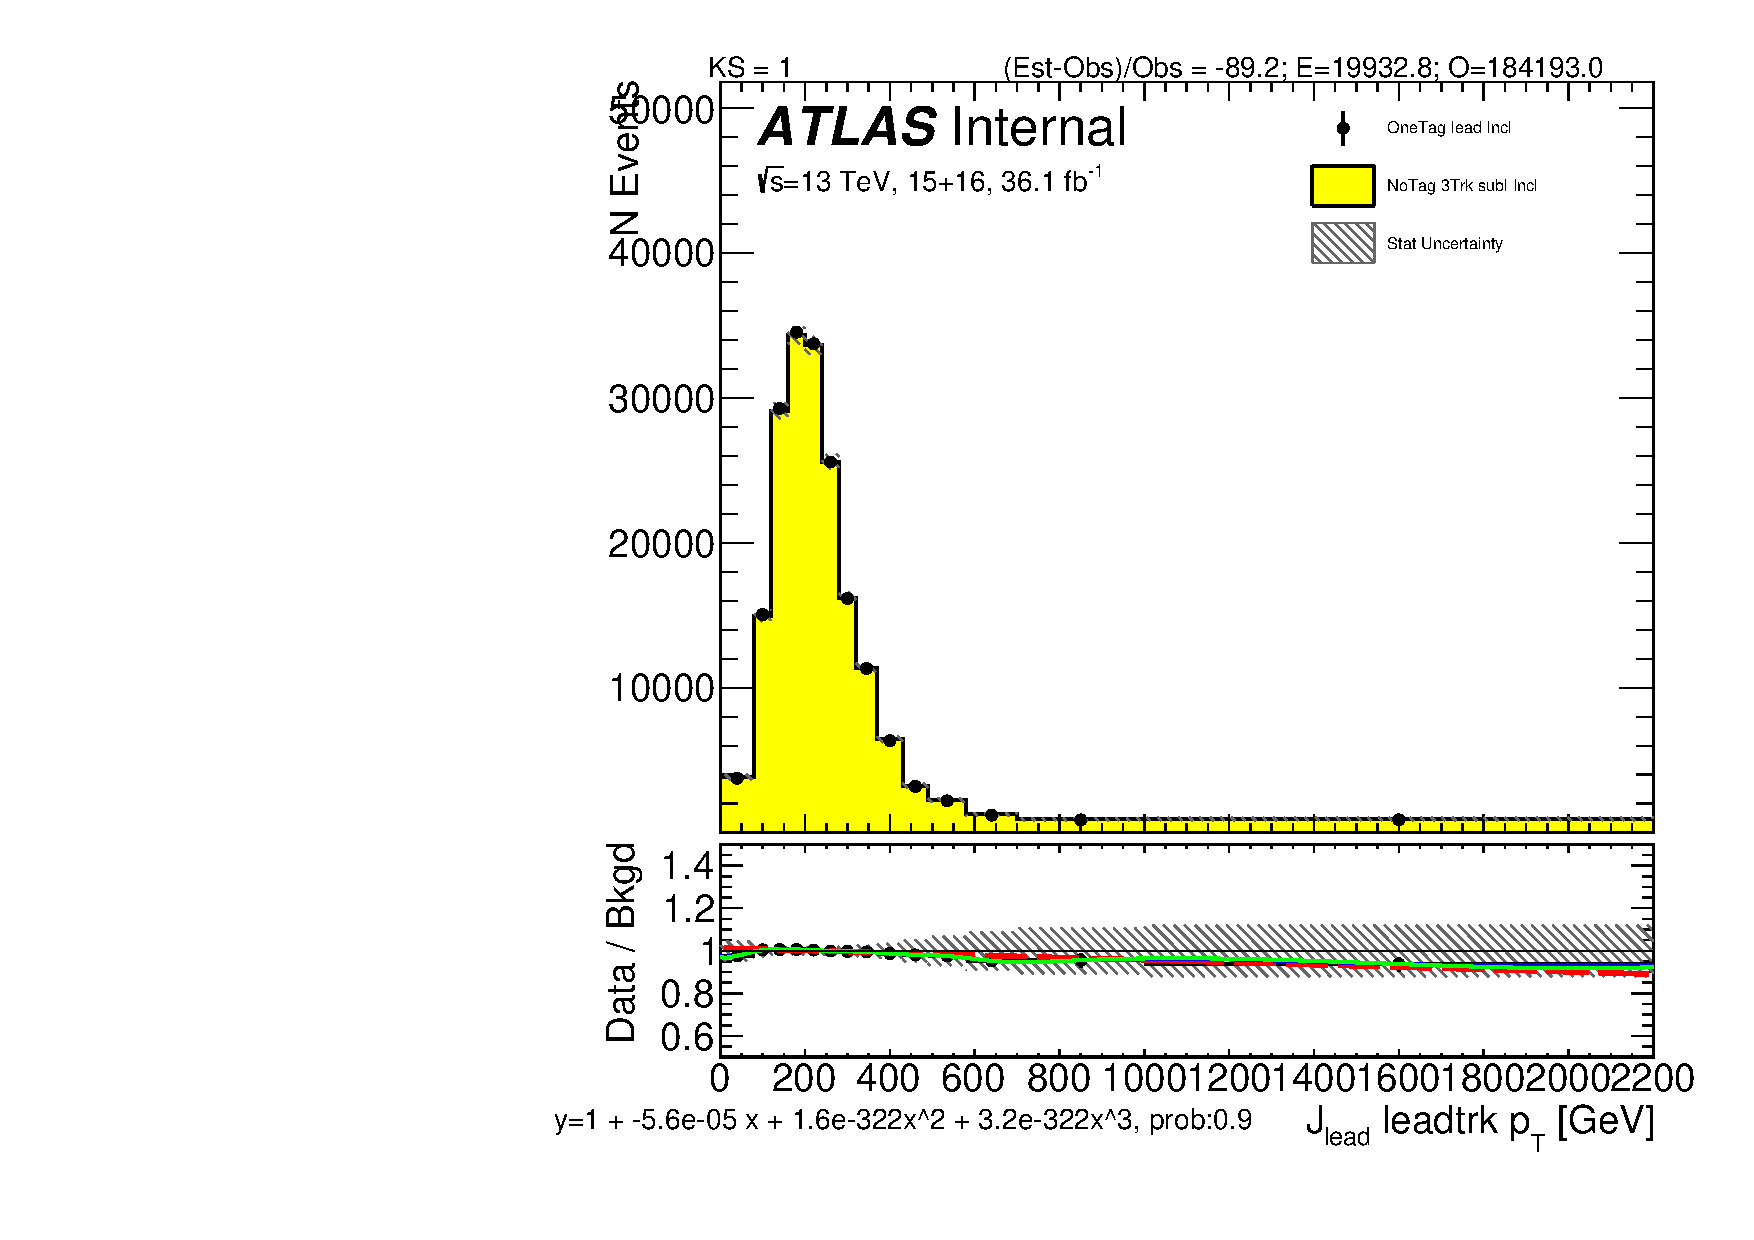
\includegraphics[width=0.25\textwidth,angle=-90]{figures/boosted/Reweight/Fits/Moriond_bkg_3_NoTag_3Trk_subl_Incl_leadHCand_trk0_Pt.pdf}
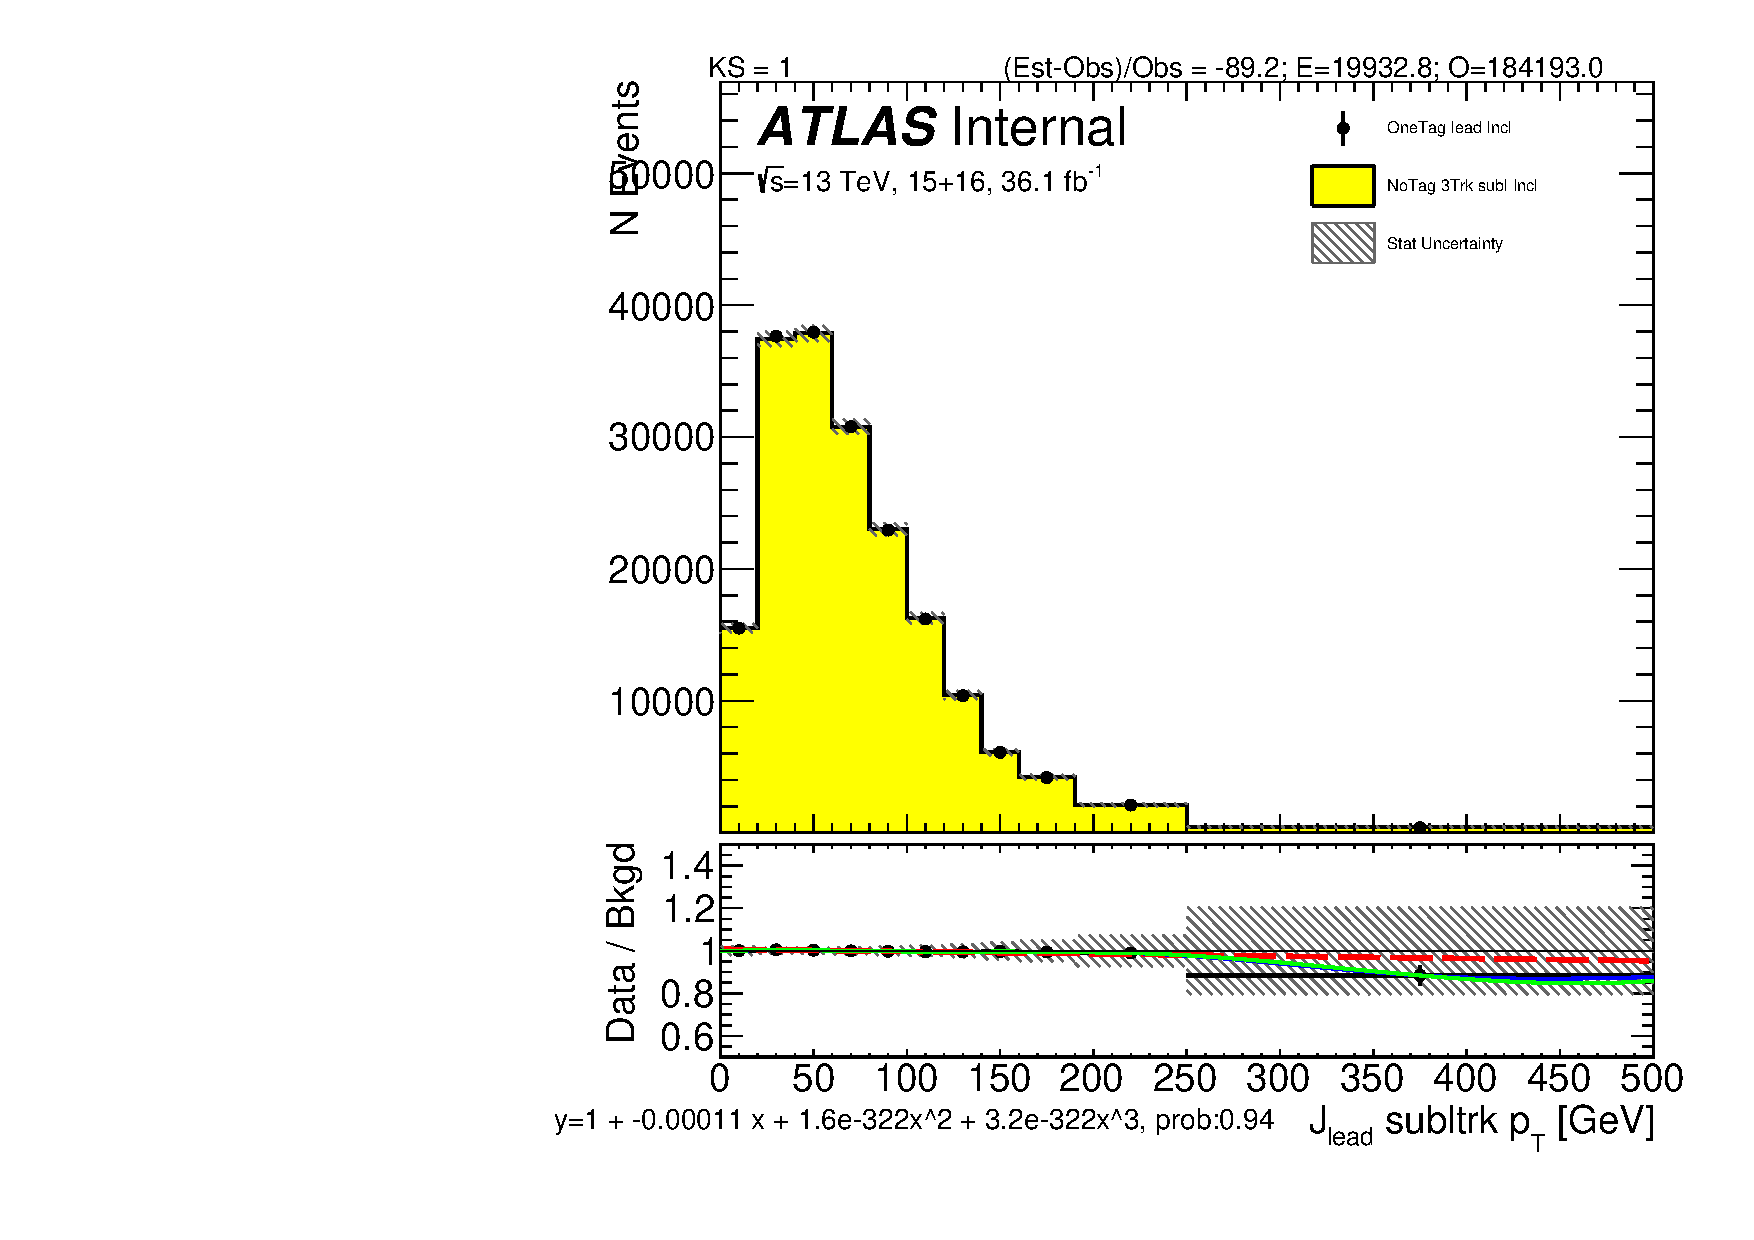
\includegraphics[width=0.25\textwidth,angle=-90]{figures/boosted/Reweight/Fits/Moriond_bkg_3_NoTag_3Trk_subl_Incl_leadHCand_trk1_Pt.pdf} \\
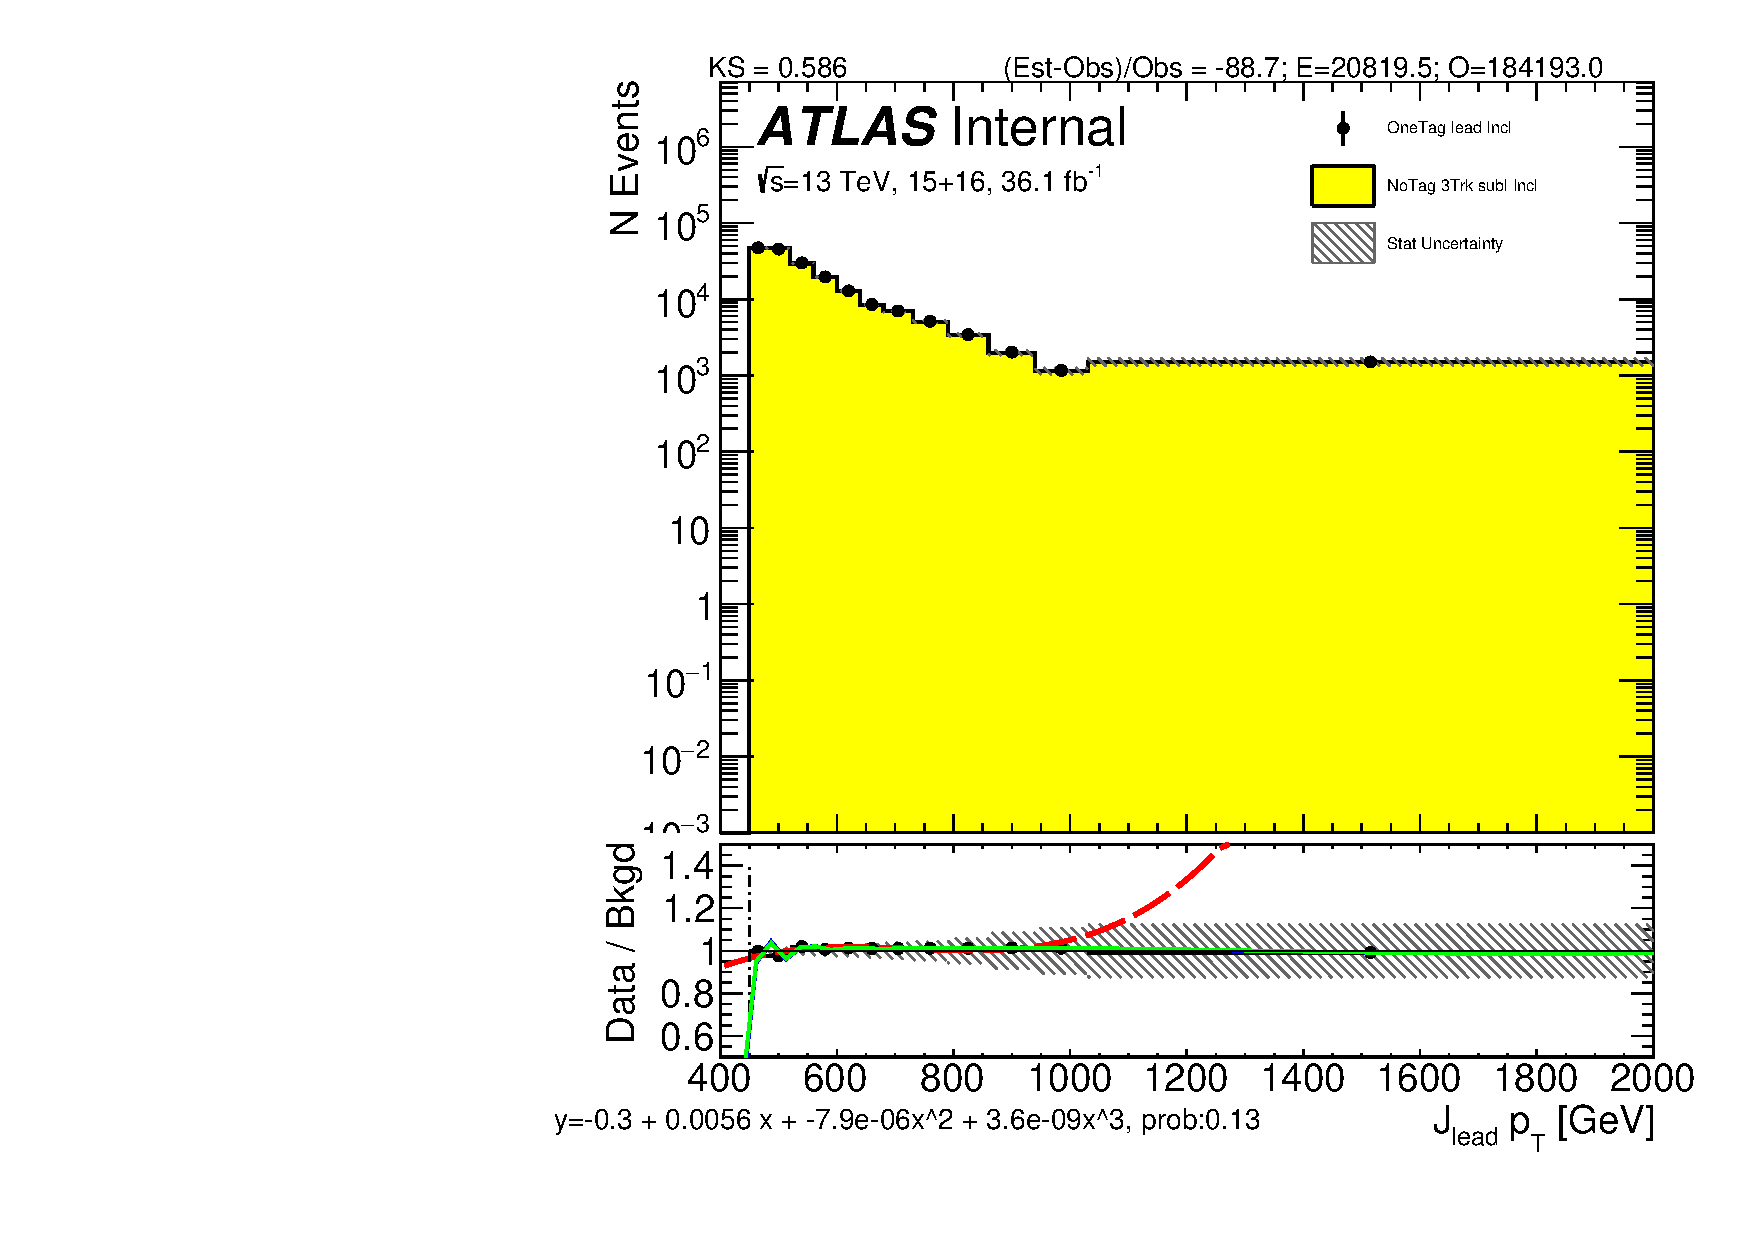
\includegraphics[width=0.25\textwidth,angle=-90]{figures/boosted/Reweight/Fits/Moriond_bkg_9_NoTag_3Trk_subl_Incl_leadHCand_Pt_m_1.pdf}
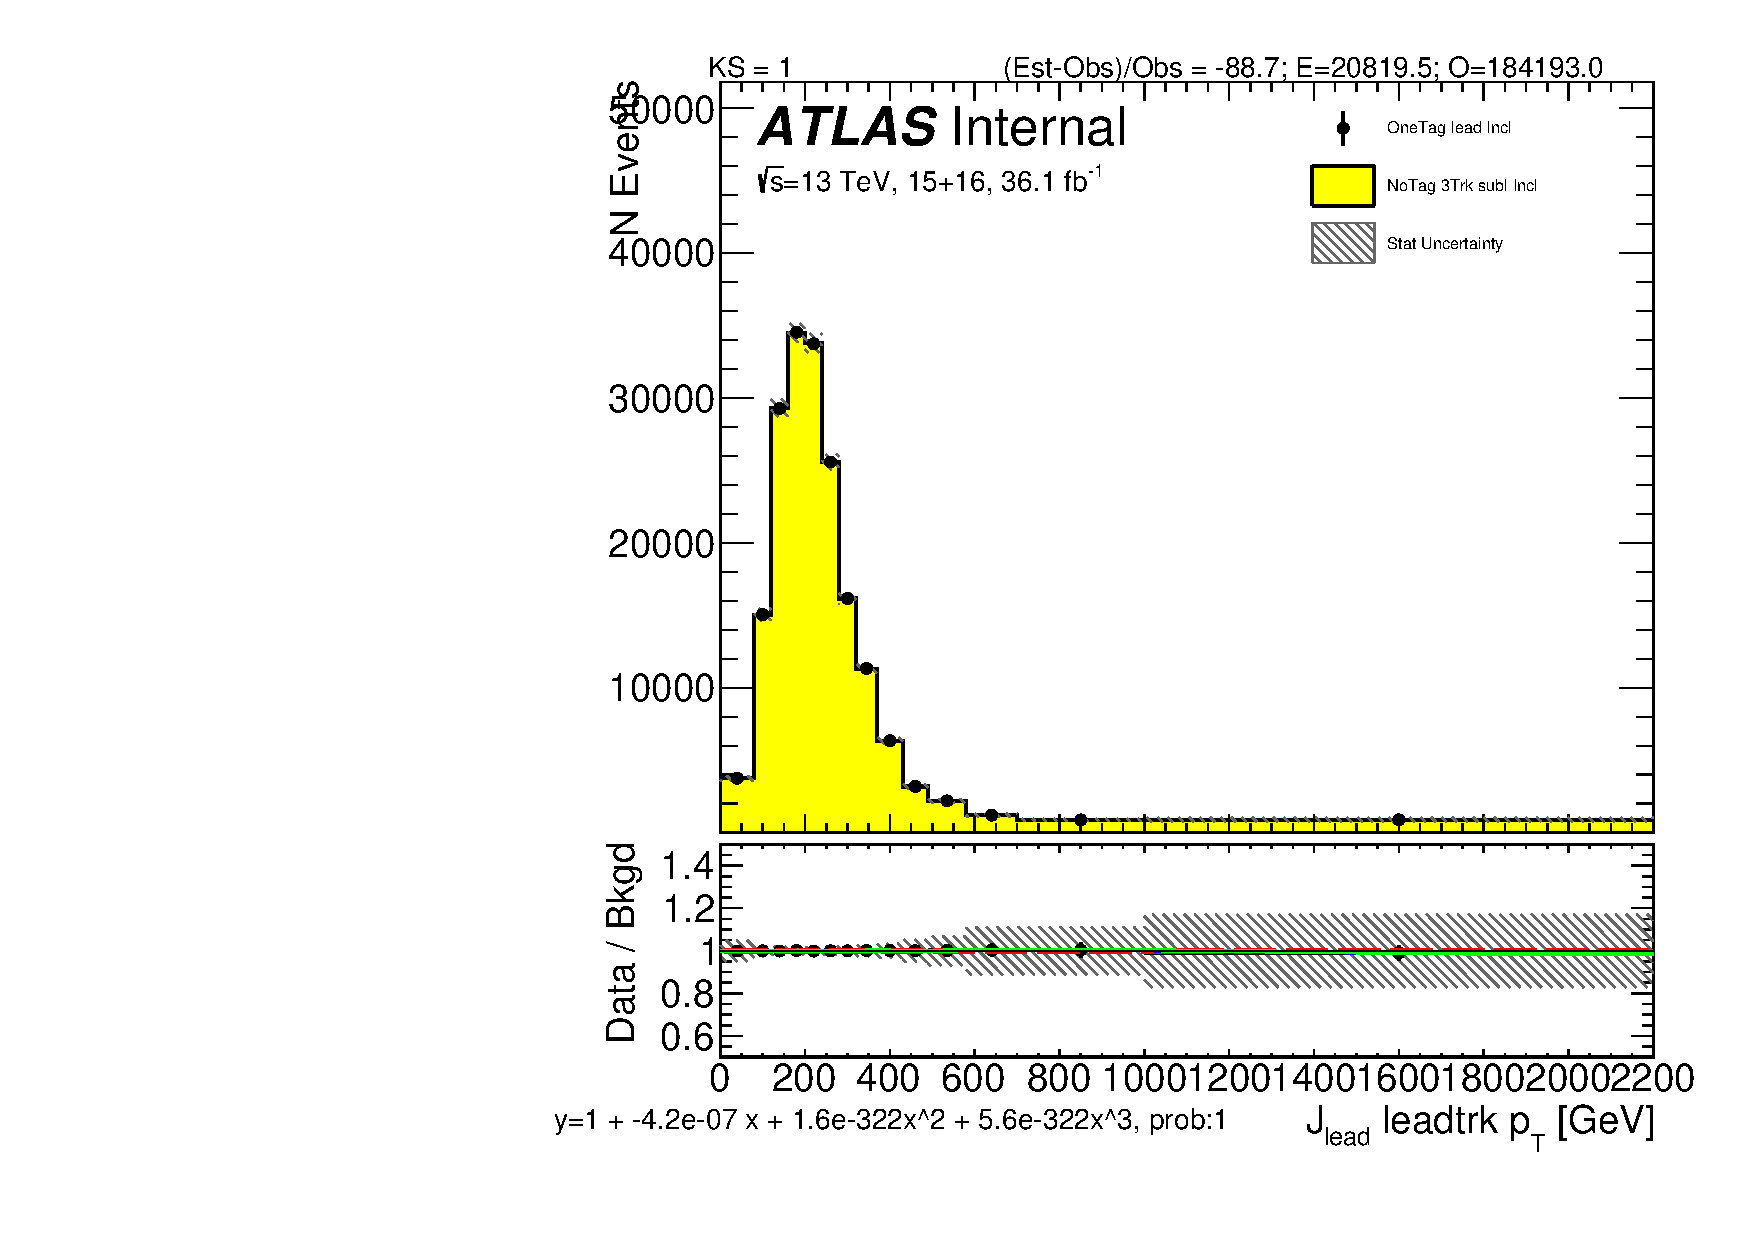
\includegraphics[width=0.25\textwidth,angle=-90]{figures/boosted/Reweight/Fits/Moriond_bkg_9_NoTag_3Trk_subl_Incl_leadHCand_trk0_Pt.pdf}
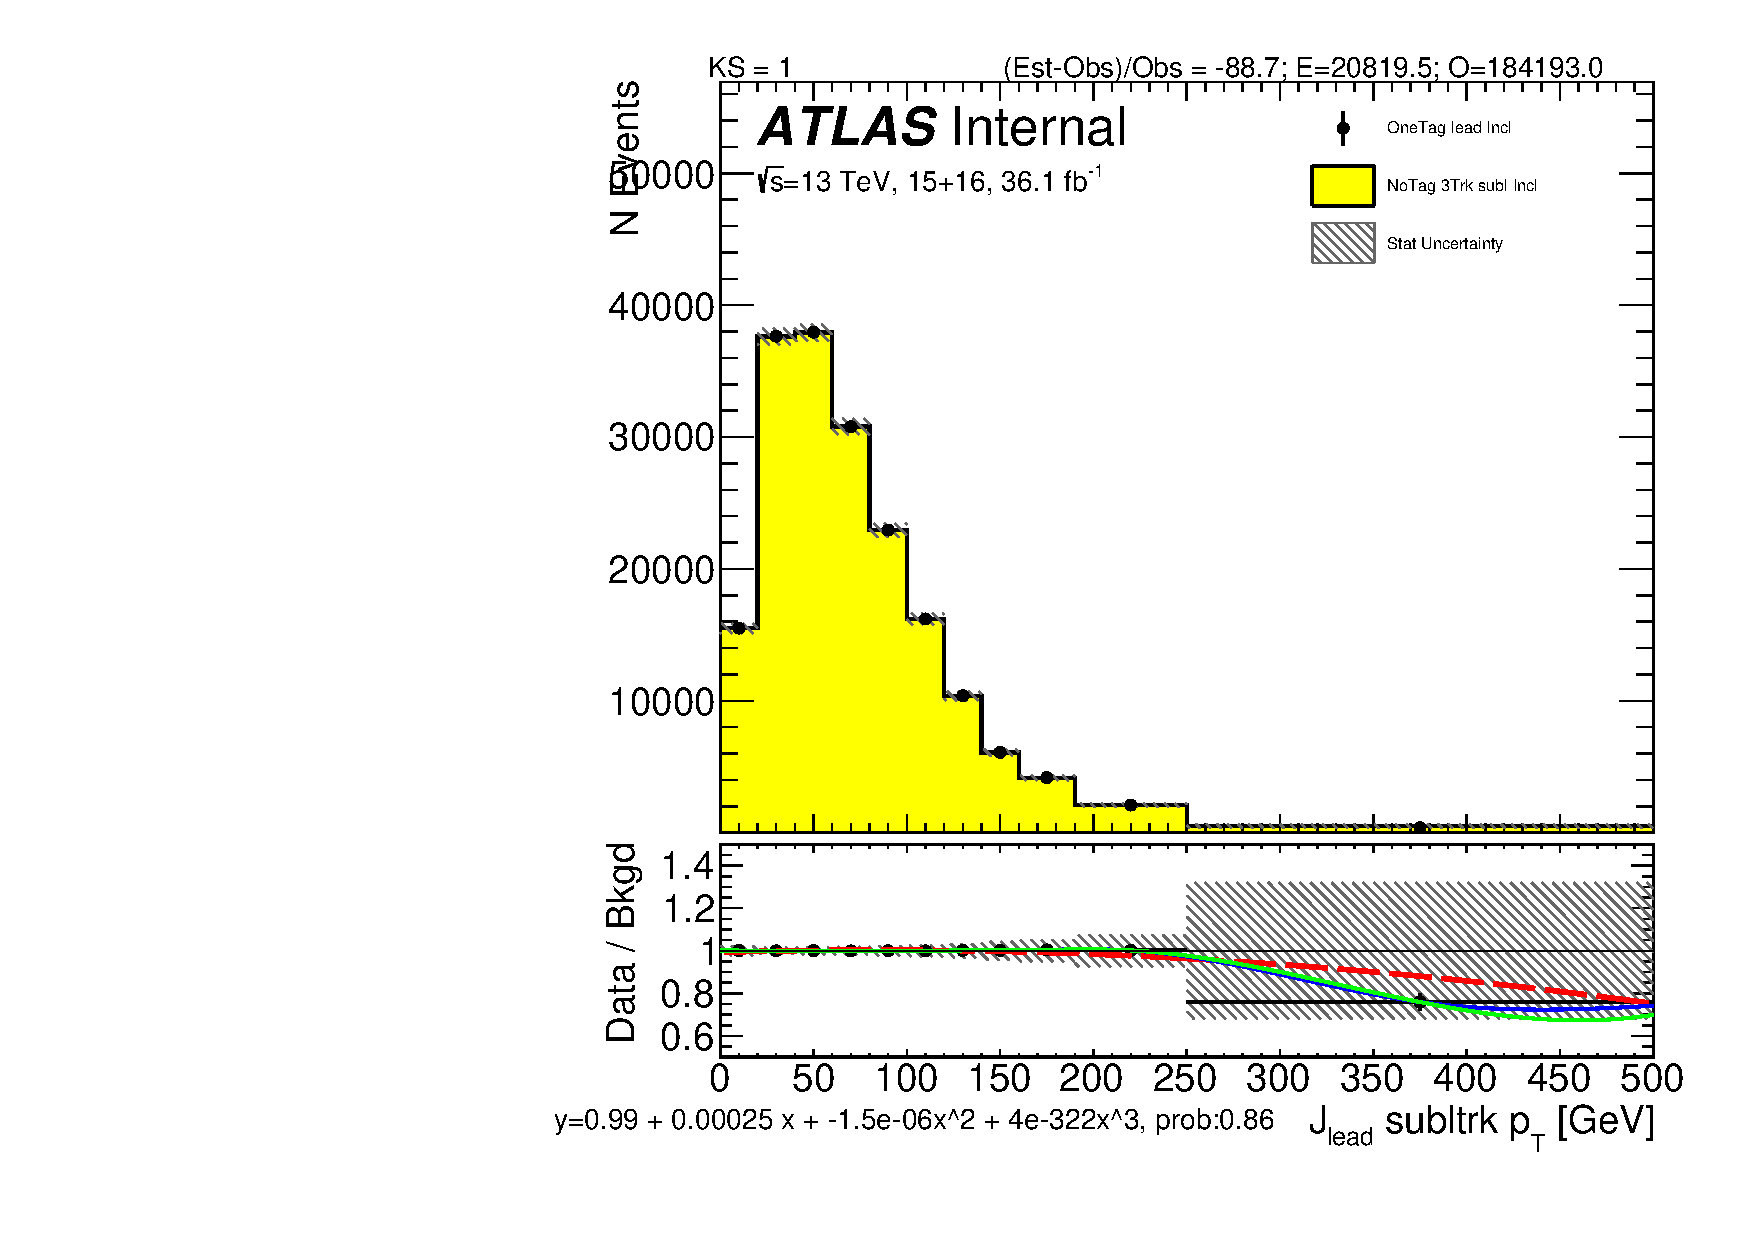
\includegraphics[width=0.25\textwidth,angle=-90]{figures/boosted/Reweight/Fits/Moriond_bkg_9_NoTag_3Trk_subl_Incl_leadHCand_trk1_Pt.pdf} \\
\caption{For $3b$ background estimate: the fits to the ratio of the data in the $2b$ category, of the leading Higgs candidate $2b$-tagged events's leading Higgs candidate distributions(black point), over the subleading Higgs candidate $1b$-tagged events's leading Higgs candidate distributions(yellow). Distributions and fits to the estimated QCD background for large-\R jet $p_{T}$ (left),  the large-\R jet's leading trackjet $p_T$ (middle), and large-\R jet's subleading trackjet $p_T$ (right) are shown.  Figures are before reweighting (top row), after the first iteration(second row), after the fourth iteration(third row), and after the last iteration (bottom row). The green line is the spline fit; the red line is a polynomial fit; the blue line is the spline interpolation.}
\label{fig:rw-3b-subl}
\end{center}
\end{figure*}

\begin{figure*}[htbp!]
\begin{center}
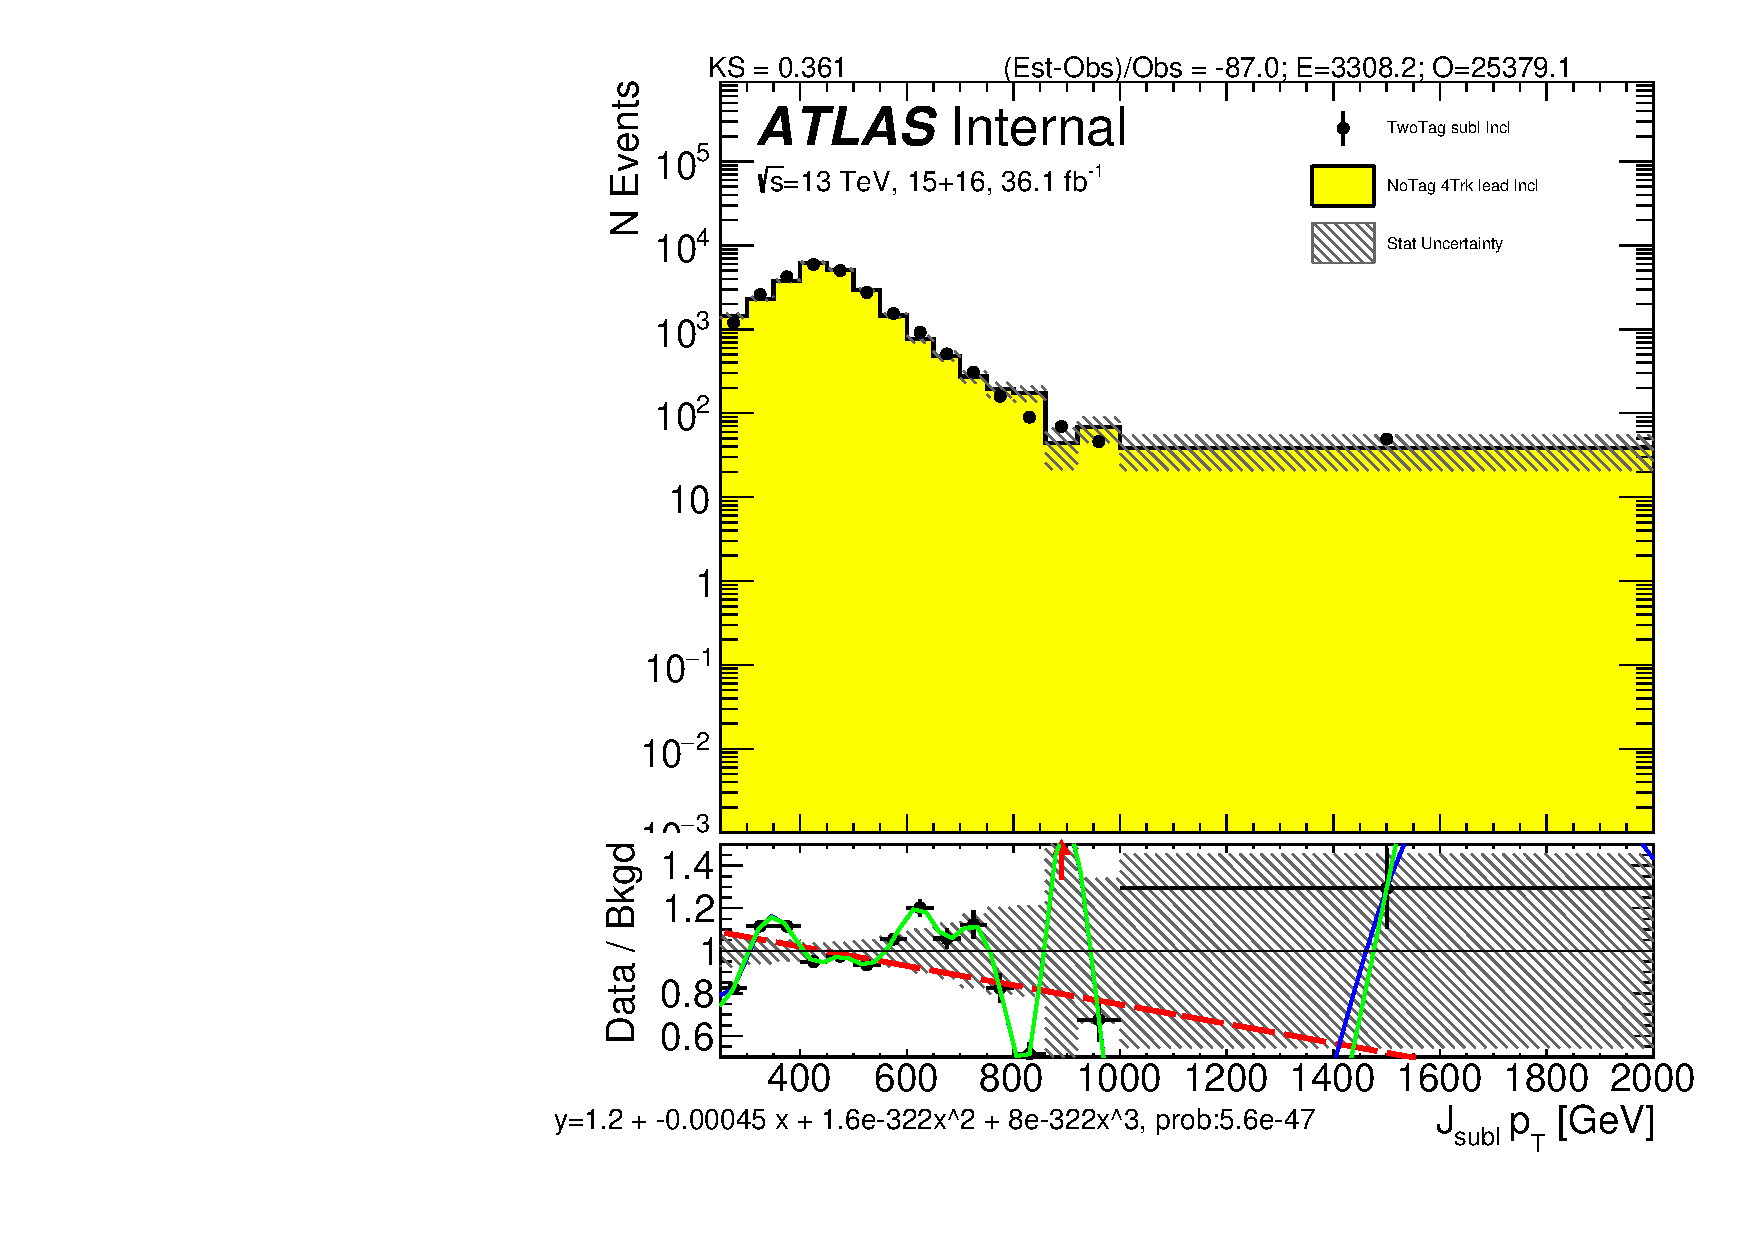
\includegraphics[width=0.25\textwidth,angle=-90]{figures/boosted/Reweight/Fits/Moriond_NoTag_4Trk_lead_Incl_sublHCand_Pt_m_1.pdf}
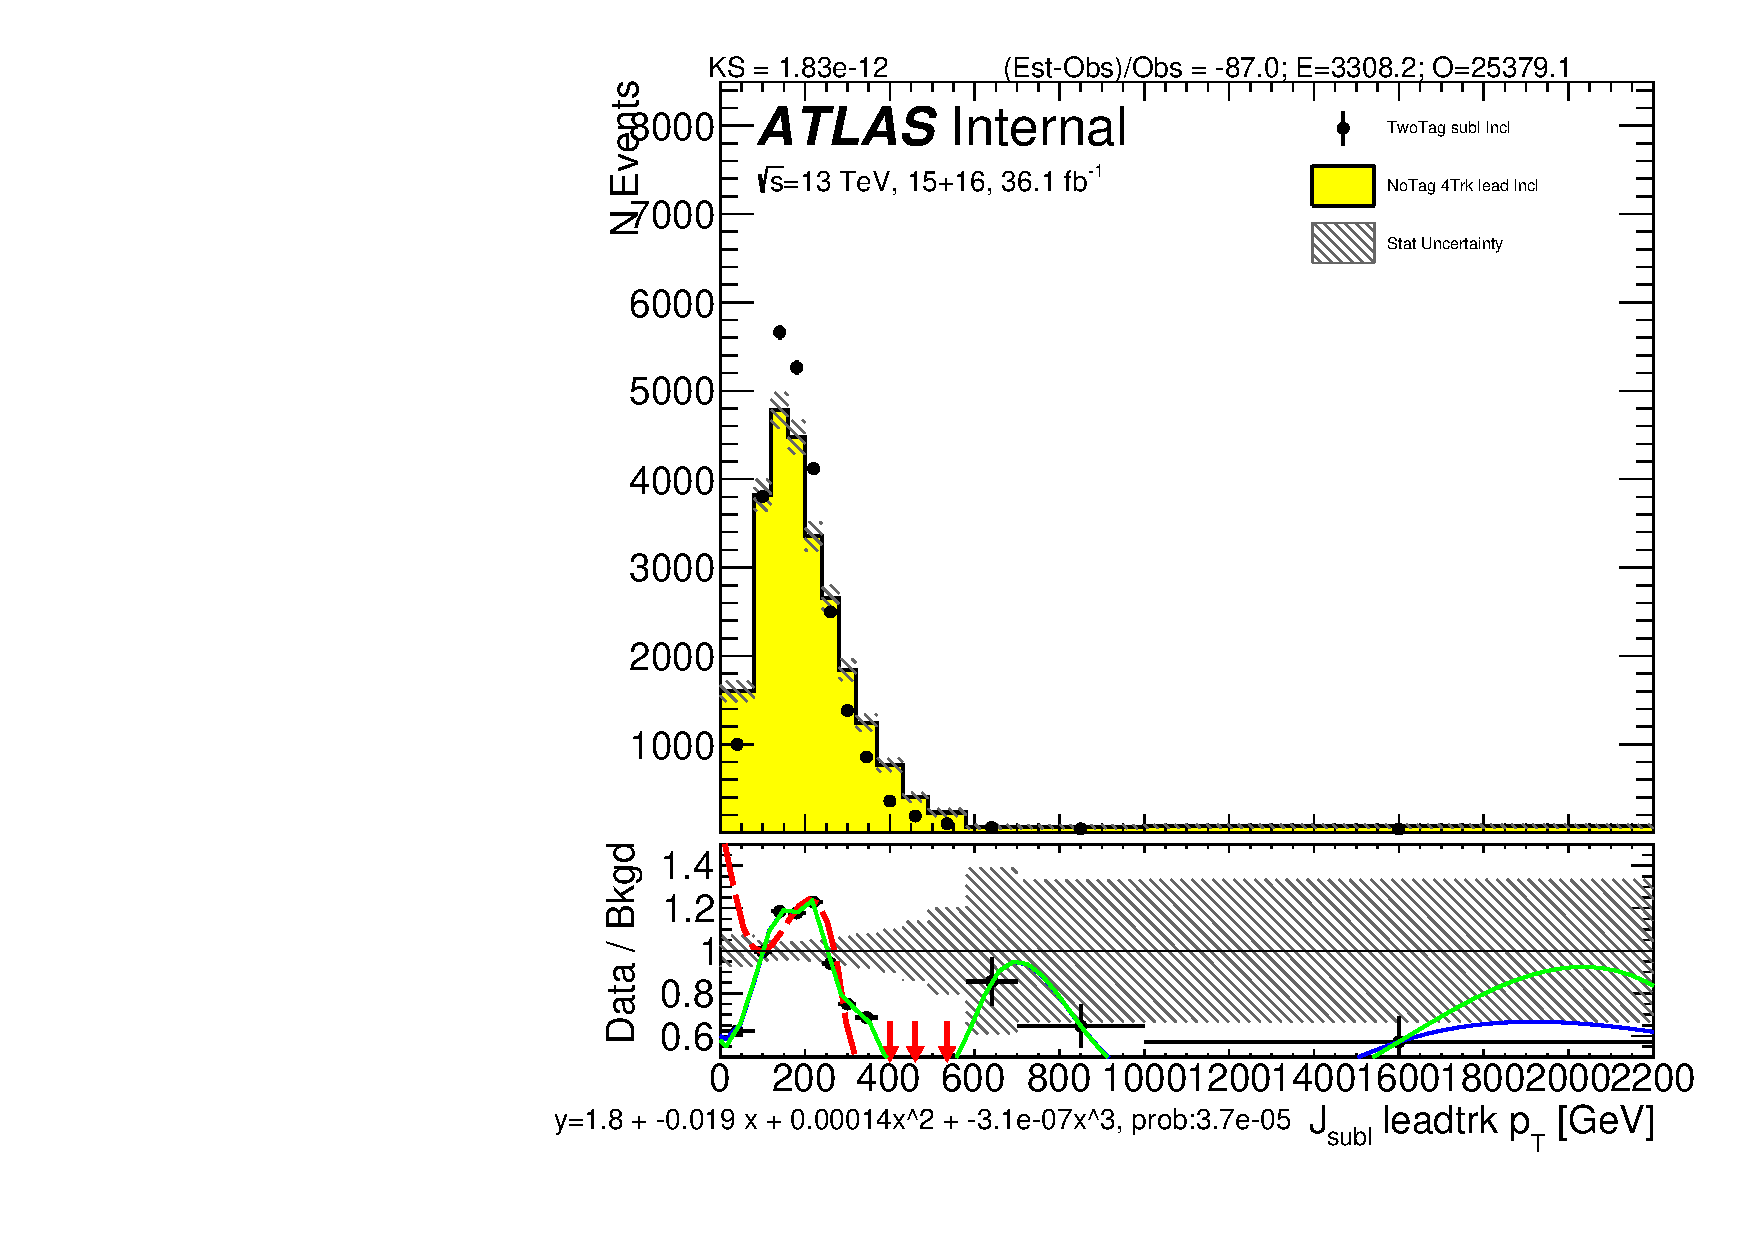
\includegraphics[width=0.25\textwidth,angle=-90]{figures/boosted/Reweight/Fits/Moriond_NoTag_4Trk_lead_Incl_sublHCand_trk0_Pt.pdf}
\includegraphics[width=0.25\textwidth,angle=-90]{figures/boosted/Reweight/Fits/Moriond_NoTag_4Trk_lead_Incl_sublHCand_trk1_Pt.pdf} \\
\includegraphics[width=0.25\textwidth,angle=-90]{figures/boosted/Reweight/Fits/Moriond_bkg_0_NoTag_4Trk_lead_Incl_sublHCand_Pt_m_1.pdf}
\includegraphics[width=0.25\textwidth,angle=-90]{figures/boosted/Reweight/Fits/Moriond_bkg_0_NoTag_4Trk_lead_Incl_sublHCand_trk0_Pt.pdf}
\includegraphics[width=0.25\textwidth,angle=-90]{figures/boosted/Reweight/Fits/Moriond_bkg_0_NoTag_4Trk_lead_Incl_sublHCand_trk1_Pt.pdf} \\
\includegraphics[width=0.25\textwidth,angle=-90]{figures/boosted/Reweight/Fits/Moriond_bkg_3_NoTag_4Trk_lead_Incl_sublHCand_Pt_m_1.pdf}
\includegraphics[width=0.25\textwidth,angle=-90]{figures/boosted/Reweight/Fits/Moriond_bkg_3_NoTag_4Trk_lead_Incl_sublHCand_trk0_Pt.pdf}
\includegraphics[width=0.25\textwidth,angle=-90]{figures/boosted/Reweight/Fits/Moriond_bkg_3_NoTag_4Trk_lead_Incl_sublHCand_trk1_Pt.pdf} \\
\includegraphics[width=0.25\textwidth,angle=-90]{figures/boosted/Reweight/Fits/Moriond_bkg_9_NoTag_4Trk_lead_Incl_sublHCand_Pt_m_1.pdf}
\includegraphics[width=0.25\textwidth,angle=-90]{figures/boosted/Reweight/Fits/Moriond_bkg_9_NoTag_4Trk_lead_Incl_sublHCand_trk0_Pt.pdf}
\includegraphics[width=0.25\textwidth,angle=-90]{figures/boosted/Reweight/Fits/Moriond_bkg_9_NoTag_4Trk_lead_Incl_sublHCand_trk1_Pt.pdf} \\
\caption{For $4b$ background estimate: the fits to the ratio of the data in the $2b$ category, of the subleading Higgs candidate $2b$-tagged events's subleading Higgs candidate distributions(black point), over the leading Higgs candidate $2b$-tagged events's subleading Higgs candidate distributions(yellow). Distributions and fits to the estimated QCD background for large-\R jet $p_{T}$ (left),  the large-\R jet's leading trackjet $p_T$ (middle), and large-\R jet's subleading trackjet $p_T$ (right) are shown.  Figures are before reweighting (top row), after the first iteration(second row), after the fourth iteration(third row), and after the last iteration (bottom row). The green line is the spline fit; the red line is a polynomial fit; the blue line is the spline interpolation.}
\label{fig:rw-4b-lead}
\end{center}
\end{figure*}

\begin{figure*}[htbp!]
\begin{center}
\includegraphics[width=0.25\textwidth,angle=-90]{figures/boosted/Reweight/Fits/Moriond_NoTag_4Trk_subl_Incl_leadHCand_Pt_m_1.pdf}
\includegraphics[width=0.25\textwidth,angle=-90]{figures/boosted/Reweight/Fits/Moriond_NoTag_4Trk_subl_Incl_leadHCand_trk0_Pt.pdf}
\includegraphics[width=0.25\textwidth,angle=-90]{figures/boosted/Reweight/Fits/Moriond_NoTag_4Trk_subl_Incl_leadHCand_trk1_Pt.pdf} \\
\includegraphics[width=0.25\textwidth,angle=-90]{figures/boosted/Reweight/Fits/Moriond_bkg_0_NoTag_4Trk_subl_Incl_leadHCand_Pt_m_1.pdf}
\includegraphics[width=0.25\textwidth,angle=-90]{figures/boosted/Reweight/Fits/Moriond_bkg_0_NoTag_4Trk_subl_Incl_leadHCand_trk0_Pt.pdf}
\includegraphics[width=0.25\textwidth,angle=-90]{figures/boosted/Reweight/Fits/Moriond_bkg_0_NoTag_4Trk_subl_Incl_leadHCand_trk1_Pt.pdf} \\
\includegraphics[width=0.25\textwidth,angle=-90]{figures/boosted/Reweight/Fits/Moriond_bkg_3_NoTag_4Trk_subl_Incl_leadHCand_Pt_m_1.pdf}
\includegraphics[width=0.25\textwidth,angle=-90]{figures/boosted/Reweight/Fits/Moriond_bkg_3_NoTag_4Trk_subl_Incl_leadHCand_trk0_Pt.pdf}
\includegraphics[width=0.25\textwidth,angle=-90]{figures/boosted/Reweight/Fits/Moriond_bkg_3_NoTag_4Trk_subl_Incl_leadHCand_trk1_Pt.pdf} \\
\includegraphics[width=0.25\textwidth,angle=-90]{figures/boosted/Reweight/Fits/Moriond_bkg_9_NoTag_4Trk_subl_Incl_leadHCand_Pt_m_1.pdf}
\includegraphics[width=0.25\textwidth,angle=-90]{figures/boosted/Reweight/Fits/Moriond_bkg_9_NoTag_4Trk_subl_Incl_leadHCand_trk0_Pt.pdf}
\includegraphics[width=0.25\textwidth,angle=-90]{figures/boosted/Reweight/Fits/Moriond_bkg_9_NoTag_4Trk_subl_Incl_leadHCand_trk1_Pt.pdf} \\
\caption{For $4b$ background estimate: the fits to the ratio of the data in the $2b$ category, of the leading Higgs candidate $2b$-tagged events's leading Higgs candidate distributions(black point), over the subleading Higgs candidate $2b$-tagged events's leading Higgs candidate distributions(yellow). Distributions and fits to the estimated QCD background for large-\R jet $p_{T}$ (left),  the large-\R jet's leading trackjet $p_T$ (middle), and large-\R jet's subleading trackjet $p_T$ (right) are shown.  Figures are before reweighting (top row), after the first iteration(second row), after the fourth iteration(third row), and after the last iteration (bottom row). The green line is the spline fit; the red line is a polynomial fit; the blue line is the spline interpolation.}
\label{fig:rw-4b-subl}
\end{center}
\end{figure*}


\paragraph{}
A comparison of the SB shapes before and after reweighting for $2bs$, $3b$ and $4b$ are shown in Figures~\ref{fig:rw-2bs-comp-sb},~\ref{fig:rw-3b-comp-sb}, and ~\ref{fig:rw-4b-comp-sb}. 
Also, a comparison of the CR shapes before and after reweighting for $2bs$, $3b$ and $4b$ can be seen in Figures~\ref{fig:rw-2bs-comp-cr},~\ref{fig:rw-3b-comp-cr}, and ~\ref{fig:rw-4b-comp-cr}. 
In almost all cases, both the reweighted/non-reweighted prediction agrees fairly well with the data, and the reweighted plots' KS scores are greater than those from non-reweighted distributions. 
%%%%%%%%%%%%%%%%%%%%%%%%%%%
\begin{figure*}[htbp!]
\begin{center}
\includegraphics[width=0.31\textwidth,angle=-90]{figures/boosted/Prereweight/Moriond_TwoTag_split_Sideband_mHH_l_1.pdf}
\includegraphics[width=0.31\textwidth,angle=-90]{figures/boosted/Sideband/b77_TwoTag_split_Sideband_mHH_l_1.pdf}\\
\includegraphics[width=0.31\textwidth,angle=-90]{figures/boosted/Prereweight/Moriond_TwoTag_split_Sideband_leadHCand_Pt_m.pdf}
\includegraphics[width=0.31\textwidth,angle=-90]{figures/boosted/Sideband/b77_TwoTag_split_Sideband_leadHCand_Pt_m.pdf}\\
\includegraphics[width=0.31\textwidth,angle=-90]{figures/boosted/Prereweight/Moriond_TwoTag_split_Sideband_leadHCand_trk0_Pt.pdf}
\includegraphics[width=0.31\textwidth,angle=-90]{figures/boosted/Sideband/b77_TwoTag_split_Sideband_leadHCand_trk0_Pt.pdf}\\
\includegraphics[width=0.31\textwidth,angle=-90]{figures/boosted/Prereweight/Moriond_TwoTag_split_Sideband_sublHCand_trk0_Pt.pdf}
\includegraphics[width=0.31\textwidth,angle=-90]{figures/boosted/Sideband/b77_TwoTag_split_Sideband_sublHCand_trk0_Pt.pdf}\\
\caption{Reweighed $2bs$ sideband region predictions comparison. Top row is the dijet Mass, second row is leading large-\R jet $p_{T}$, third row is the leading large-\R jet's leading trackjet $p_T$ and the last row subleading large-\R jet's leading trackjet $p_T$. On the left are the distributions before reweighting, and on the right are the distributions after reweighting.}
\label{fig:rw-2bs-comp-sb}
\end{center}
\end{figure*}


\begin{figure*}[htbp!]
\begin{center}
\includegraphics[width=0.31\textwidth,angle=-90]{figures/boosted/Prereweight/Moriond_ThreeTag_Sideband_mHH_l_1.pdf}
\includegraphics[width=0.31\textwidth,angle=-90]{figures/boosted/Sideband/b77_ThreeTag_Sideband_mHH_l_1.pdf}\\
\includegraphics[width=0.31\textwidth,angle=-90]{figures/boosted/Prereweight/Moriond_ThreeTag_Sideband_leadHCand_Pt_m.pdf}
\includegraphics[width=0.31\textwidth,angle=-90]{figures/boosted/Sideband/b77_ThreeTag_Sideband_leadHCand_Pt_m.pdf}\\
\includegraphics[width=0.31\textwidth,angle=-90]{figures/boosted/Prereweight/Moriond_ThreeTag_Sideband_leadHCand_trk0_Pt.pdf}
\includegraphics[width=0.31\textwidth,angle=-90]{figures/boosted/Sideband/b77_ThreeTag_Sideband_leadHCand_trk0_Pt.pdf}\\
\includegraphics[width=0.31\textwidth,angle=-90]{figures/boosted/Prereweight/Moriond_ThreeTag_Sideband_sublHCand_trk0_Pt.pdf}
\includegraphics[width=0.31\textwidth,angle=-90]{figures/boosted/Sideband/b77_ThreeTag_Sideband_sublHCand_trk0_Pt.pdf}\\
\caption{Reweighed $3b$ sideband region predictions comparison. Top row is the dijet Mass, second row is leading large-\R jet $p_{T}$, third row is the leading large-\R jet's leading trackjet $p_T$ and the last row subleading large-\R jet's leading trackjet $p_T$. On the left are the distributions before reweighting, and on the right are the distributions after reweighting.}
\label{fig:rw-3b-comp-sb}
\end{center}
\end{figure*}


\begin{figure*}[htbp!]
\begin{center}
\includegraphics[width=0.31\textwidth,angle=-90]{figures/boosted/Prereweight/Moriond_FourTag_Sideband_mHH_l_1.pdf}
\includegraphics[width=0.31\textwidth,angle=-90]{figures/boosted/Sideband/b77_FourTag_Sideband_mHH_l_1.pdf}\\
\includegraphics[width=0.31\textwidth,angle=-90]{figures/boosted/Prereweight/Moriond_FourTag_Sideband_leadHCand_Pt_m.pdf}
\includegraphics[width=0.31\textwidth,angle=-90]{figures/boosted/Sideband/b77_FourTag_Sideband_leadHCand_Pt_m.pdf}\\
\includegraphics[width=0.31\textwidth,angle=-90]{figures/boosted/Prereweight/Moriond_FourTag_Sideband_leadHCand_trk0_Pt.pdf}
\includegraphics[width=0.31\textwidth,angle=-90]{figures/boosted/Sideband/b77_FourTag_Sideband_leadHCand_trk0_Pt.pdf}\\
\includegraphics[width=0.31\textwidth,angle=-90]{figures/boosted/Prereweight/Moriond_FourTag_Sideband_sublHCand_trk0_Pt.pdf}
\includegraphics[width=0.31\textwidth,angle=-90]{figures/boosted/Sideband/b77_FourTag_Sideband_sublHCand_trk0_Pt.pdf}\\
\caption{Reweighted $4b$ sideband region predictions comaprison. Top row is the dijet Mass, second row is leading large-\R jet $p_{T}$, third row is the leading large-\R jet's leading trackjet $p_T$ and the last row subleading large-\R jet's leading trackjet $p_T$. On the left are the distributions before reweighting, and on the right are the distributions after reweighting.}
\label{fig:rw-4b-comp-sb}
\end{center}
\end{figure*}


\begin{figure*}[htbp!]
\begin{center}
\includegraphics[width=0.31\textwidth,angle=-90]{figures/boosted/Prereweight/Moriond_TwoTag_split_Control_mHH_l_1.pdf}
\includegraphics[width=0.31\textwidth,angle=-90]{figures/boosted/Control/b77_TwoTag_split_Control_mHH_l_1.pdf}\\
\includegraphics[width=0.31\textwidth,angle=-90]{figures/boosted/Prereweight/Moriond_TwoTag_split_Control_leadHCand_Pt_m.pdf}
\includegraphics[width=0.31\textwidth,angle=-90]{figures/boosted/Control/b77_TwoTag_split_Control_leadHCand_Pt_m.pdf}\\
\includegraphics[width=0.31\textwidth,angle=-90]{figures/boosted/Prereweight/Moriond_TwoTag_split_Control_leadHCand_trk0_Pt.pdf}
\includegraphics[width=0.31\textwidth,angle=-90]{figures/boosted/Control/b77_TwoTag_split_Control_leadHCand_trk0_Pt.pdf}\\
\includegraphics[width=0.31\textwidth,angle=-90]{figures/boosted/Prereweight/Moriond_TwoTag_split_Control_sublHCand_trk0_Pt.pdf}
\includegraphics[width=0.31\textwidth,angle=-90]{figures/boosted/Control/b77_TwoTag_split_Control_sublHCand_trk0_Pt.pdf}\\
\caption{Reweighted $2bs$ control region predictions comaprison. Top row is the dijet Mass, second row is leading large-\R jet $p_{T}$, third row is the leading large-\R jet's leading trackjet $p_T$ and the last row subleading large-\R jet's leading trackjet $p_T$. On the left are the distributions before reweighting, and on the right are the distributions after reweighting.}
\label{fig:rw-2bs-comp-cr}
\end{center}
\end{figure*}


\begin{figure*}[htbp!]
\begin{center}
\includegraphics[width=0.31\textwidth,angle=-90]{figures/boosted/Prereweight/Moriond_ThreeTag_Control_mHH_l_1.pdf}
\includegraphics[width=0.31\textwidth,angle=-90]{figures/boosted/Control/b77_ThreeTag_Control_mHH_l_1.pdf}\\
\includegraphics[width=0.31\textwidth,angle=-90]{figures/boosted/Prereweight/Moriond_ThreeTag_Control_leadHCand_Pt_m.pdf}
\includegraphics[width=0.31\textwidth,angle=-90]{figures/boosted/Control/b77_ThreeTag_Control_leadHCand_Pt_m.pdf}\\
\includegraphics[width=0.31\textwidth,angle=-90]{figures/boosted/Prereweight/Moriond_ThreeTag_Control_leadHCand_trk0_Pt.pdf}
\includegraphics[width=0.31\textwidth,angle=-90]{figures/boosted/Control/b77_ThreeTag_Control_leadHCand_trk0_Pt.pdf}\\
\includegraphics[width=0.31\textwidth,angle=-90]{figures/boosted/Prereweight/Moriond_ThreeTag_Control_sublHCand_trk0_Pt.pdf}
\includegraphics[width=0.31\textwidth,angle=-90]{figures/boosted/Control/b77_ThreeTag_Control_sublHCand_trk0_Pt.pdf}\\
\caption{Reweighted $3b$ control region predictions comaprison. Top row is the dijet Mass, second row is leading large-\R jet $p_{T}$, third row is the leading large-\R jet's leading trackjet $p_T$ and the last row subleading large-\R jet's leading trackjet $p_T$. On the left are the distributions before reweighting, and on the right are the distributions after reweighting.}
\label{fig:rw-3b-comp-cr}
\end{center}
\end{figure*}


\begin{figure*}[htbp!]
\begin{center}
\includegraphics[width=0.31\textwidth,angle=-90]{figures/boosted/Prereweight/Moriond_FourTag_Control_mHH_l_1.pdf}
\includegraphics[width=0.31\textwidth,angle=-90]{figures/boosted/Control/b77_FourTag_Control_mHH_l_1.pdf}\\
\includegraphics[width=0.31\textwidth,angle=-90]{figures/boosted/Prereweight/Moriond_FourTag_Control_leadHCand_Pt_m.pdf}
\includegraphics[width=0.31\textwidth,angle=-90]{figures/boosted/Control/b77_FourTag_Control_leadHCand_Pt_m.pdf}\\
\includegraphics[width=0.31\textwidth,angle=-90]{figures/boosted/Prereweight/Moriond_FourTag_Control_leadHCand_trk0_Pt.pdf}
\includegraphics[width=0.31\textwidth,angle=-90]{figures/boosted/Control/b77_FourTag_Control_leadHCand_trk0_Pt.pdf}\\
\includegraphics[width=0.31\textwidth,angle=-90]{figures/boosted/Prereweight/Moriond_FourTag_Control_sublHCand_trk0_Pt.pdf}
\includegraphics[width=0.31\textwidth,angle=-90]{figures/boosted/Control/b77_FourTag_Control_sublHCand_trk0_Pt.pdf}\\
\caption{Reweighted $4b$ control region predictions comaprison. Top row is the dijet Mass, second row is leading large-\R jet $p_{T}$, third row is the leading large-\R jet's leading trackjet $p_T$ and the last row subleading large-\R jet's leading trackjet $p_T$. On the left are the distributions before reweighting, and on the right are the distributions after reweighting.}
\label{fig:rw-4b-comp-cr}
\end{center}
\end{figure*}

